%%%%%%%%%%%%%%%%%%%%%%%%%%%%%%%%%%%%%%%%%%%%%%%%%%%%%%%%%%%%%%%%%%%
%                                                                 %
%                            ROOT FILE                            %
%                                                                 %
%%%%%%%%%%%%%%%%%%%%%%%%%%%%%%%%%%%%%%%%%%%%%%%%%%%%%%%%%%%%%%%%%%%
%
%  Run LaTeX or pdfLaTeX on this file to produce your dissertation.
%  To produce the abstract title page followed by the abstract,
%  see the file abstitle-phd.tex or abstitle-mas.tex.
%  Downloaded originally from: http://www.cs.albany.edu/Albany_LaTeX_Dissertation_Template/
%  Thanks to Ben Carle, Ph.D. 2010
% Hannah E. Attard edited in 2014 for use as a masters template for U. Albany Dept. of Atmospheric and Environmental Sciences
% Edited, trimmed and modified to work for PhD (& Masters) 2015 format 
%%%%%%%%%%%%%%%%%%%%%%%%%%%%%%%%%%%%%%%%%%%%%%%%%%%%%%%%%%%%%%%%%%%

\documentclass[]{thesis}
%%%%%%%%
\usepackage[T1]{fontenc}
\usepackage{textcomp}
\usepackage{gensymb}
%\usepackage{dcolumn}
%\usepackage{subfig}
%\usepackage{epsfig, latexsym, graphics, graphicx, url}
\usepackage{yfonts}
\usepackage{color}
\usepackage{fancyhdr}
\usepackage{natbib} %HEA 1/23/14 deleted [square,comma] 
\bibpunct[; ]{(}{)}{;}{a}{}{;} %HEA 6/3/14 added this so that references are (Jones 2001) instead of (Jones, 2001) & ; between lists of authors referenced
\usepackage[utf8]{inputenc} %HEA 1/28/14 added for special characters in .bib
\usepackage[toc, acronym]{glossaries}
\usepackage{rotating} %HEA 1/21/14 added package (for table)
\usepackage{booktabs} %HEA 1/23/14 added package (for tables)
\usepackage[hyperfootnotes=true]{hyperref} %HEA 1/27/14 added pacakge need to tablefootnote
\usepackage{threeparttable} %HEA 1/28/14 Now table footnotes work.  Keeping the other packages for future
\usepackage{footnotebackref}
\usepackage{tablefootnote} %HEA 1/27/14 added package (for tables!)
%\usepackage[noeepic]{qtree}
%%%%%%%%

\bibpunct{(}{)}{;}{a}{}{,}

%\documentclass{ametsoc}
%\usepackage[T1]{fontenc}
%\usepackage{gensymb}
%\usepackage{dcolumn}
%\usepackage{subfig}


\usepackage{layout}
\newcommand{\mytilde}{\raise.17ex\hbox{$\scriptstyle\mathtt{\sim}$}}

\def\topline{\hline\hline\vrule height 10pt depth4pt width0pt\relax}
\def\midline{\hline\vrule height 10pt width0pt\relax}
\def\botline{\hline}

\newcommand{\red}[1]{\textcolor{red}{#1}}

%%%%%%%%%%%%%%%%%%%%%%%%%%%%%%%%%%%%%%
%%%%  Superscipt .tex line number insert
\newcommand{\ts}{\textsuperscript}
%%%%%%%%%%%%%%%%%%%%%%%%%%%%%%%%%%%%%

% \newcommand{\ignore}[1]{}
% \newcommand{\undr}{\underline}
% \newcommand{\ovr}{\overline}
% \newcommand{\flr}{\rightarrow}
% \newcommand{\fll}{\leftarrow}
% \newcommand{\fflr}{\longrightarrow}
% \newcommand{\fl}{-\!\!\!-\!\!\!-\!\!\!-\!\!\!-\!\!\!}
% \newcommand{\ffflr}{\fl\fflr}
% \newcommand{\lft}{\noindent}
% \newcommand{\Flr}{\Longrightarrow}
% \newcommand{\mFlr}{\,{|}\!\!\!\Flr}
% \newcommand{\app}{\approx}
% \newcommand{\nat}{\mathbb{N}}

% \newcommand{\proof}{{\em Proof\/}: }
% \newcommand{\qed}{\hfill $\fbox{}$}

% \newcommand{\disp}[1]{\vspace{-0.5em}\begin{center} {#1}
%                                    \end{center}\vspace{-0.5em}}
% \newcommand{\dispn}[2]{ {\noindent{#1}} \centerline{#2} }

% \newcommand{\msup}[2]{\stackrel{#2}{#1}}

% \newcommand{\h}{\bf h}

% \newcommand{\A}{\bf A}
% \newcommand{\B}{\cal B}
% \newcommand{\C}{{\cal C}}
% \newcommand{\D}{{\cal D}}
% \newcommand{\E}{{\cal E}}
% \newcommand{\F}{{\cal F}}
% \newcommand{\m}{{\cal L}}
% \newcommand{\M}{{\cal M}}
% \newcommand{\s}{{\cal S}}
% \newcommand{\U}{{\cal U}}
% \newcommand{\W}{{\cal I}}

% \newcommand{\G}{\mathcal{G}}
% \newcommand{\I}{\mathcal{I}}
% \renewcommand{\L}{\mathcal{L}}
% \renewcommand{\P}{\mathcal{P}}
% \newcommand{\Q}{\mathcal{Q}}
% \newcommand{\R}{\mathcal{R}}
% \renewcommand{\S}{\mathcal{S}}
% \newcommand{\T}{\mathcal{T}}
% \newcommand{\X}{\mathcal{X}}
% \newcommand{\cc}{{\succ\!\!\!\succ}}

% \newtheorem{theorem}{Theorem}[chapter]

% \newtheorem{propn}{Proposition}[chapter]
% \newtheorem{defn}{Definition}[chapter]
% \newtheorem{corol}{Corollary}[chapter]
% \newtheorem{lemma}{Lemma}[chapter]

% \newcommand{\hsp}{\hspace*{0.7cm}}
% \newcommand{\hsps}{\hspace*{1em}}
% \newcommand{\hspa}{\hspace*{1cm}}
% \newcommand{\hspb}{\hspace*{1.5cm}}
% \newcommand{\donno}{\,?\,}



%%%%%%%%%%%%%%%%%%%%%%%%% Title Info %%%%%%%%%%%%%%%%%%%%%%%%%
% You should replace the appropriate fields in
% the following section with your own information.

\thesistitle{\bf The upper-level turbulence, static stability and tropopause structure of tropical cyclones }
\thesissubtitle{\bf }
\author{ Patrick Timothy Duran}
\degreetype{Doctor of Philosophy}
\college{College of Arts and Sciences}
\department{Atmospheric and Environmental Sciences}
\submitdate{2018}
\copyrightyear{2018}   % if omitted, current year is used.
\dedicatedto{}
\signaturelines{5}     %More than 4 and the sig page will probably overflow. 5 if you have a short title

%%%%%%%%%%%%%%%%%%%%%%%% End Title Info %%%%%%%%%%%%%%%%%%%%%%%%%


%\graphicspath{figures/}  %directory that has the figures so you don't need path in add figures
%\makeglossaries

\newglossaryentry{eregex}{name={eregex},
description={An extended regular expression, i.e. a regular expression with the addition of backreferences}}

\newacronym{SRE}{SRE}{Synchronized Regular Expression}


\begin{document}
%\layout     %% this is helpful to check formatting

%\sigblockalb

\titlepage
%\copyrightpage

%%%%%%%%%%%%%%%%%%%%%%%%%%%%%%%%%%%%%%%%%%%%%%%%%%%%%%%%%%%%%%%%%%% 
%                                                                 %
%                            ABSTRACT                             %
%                                                                 %
%%%%%%%%%%%%%%%%%%%%%%%%%%%%%%%%%%%%%%%%%%%%%%%%%%%%%%%%%%%%%%%%%%% 
 
\specialhead{ABSTRACT}

Enter your abstract here.  %this is your abstract.tex file
%%%%%%%%%%%%%%%%%%%%%%%%%%%%%%%%%%%%%%%%%%%%%%%%%%%%%%%%%%%%%%%%%%% 
%                                                                 %
%                         ACKNOWLEDGEMENT                         %
%                                                                 %
%%%%%%%%%%%%%%%%%%%%%%%%%%%%%%%%%%%%%%%%%%%%%%%%%%%%%%%%%%%%%%%%%%% 
 
\specialhead{ACKNOWLEDGEMENTS}

%---------------------------------------------------------------------------------------%

\indent \indent This dissertation is the fulfillment of a childhood dream that would not have come true without the selfless dedication of countless people.
The list of all of the people who have helped me along the way is far too lengthy to include here, so below I acknowledge only those who were particularly influential on this journey.

First I thank my advisor, Dr. John Molinari, for his unswerving kindness, humility, and patience over these past six years.  
Former students have described him as a "brilliant scientist and an even better man," an assessment with which I wholeheartedly concur.  
I could not have asked for a better mentor, and am so grateful for the opportunities he has given to me.

I also would like to thank my committee members - Drs. Kristen Corbosiero, Robert Fovell, Brian Tang, and Ryan Torn - for their guidance and support over these years.  
Truly an academic all-star team, I will continue to look up to each of them as models of scientific brilliance.

Thanks to all of the DAES faculty for building and carefully maintaining such a positive and constructive departmental culture.  
It was always comforting to know that every faculty member truly cared about the students, and always worked to build us up as scientists and professionals.  
Nowhere was their dedication to students more evident than in their outstanding courses, which I thoroughly enjoyed, and which greatly contributed to my knowledge.  

I also owe a tremendous debt to Dr. Steven Lazarus and Michael Splitt of the Florida Institute of Technology, whose selfless investment in me as an undergraduate played a critical role in my academic development, and prepared me for PhD-level research and course work.

I am grateful for the support and friendship of all of the DAES graduate students, particularly Travis Elless, Stephanie Stevenson, Oscar Chimborazo, Steven Fuhrman, Ahmed Shaaban, Sarah Ditchek, Matthew Vaughan, Michael Fischer, Hannah Attard, Josh Alland, Chen Yuan-Ming, and Connor Nelson.  
Their friendship and encouragement over these years has meant a lot to me.
I owe a special thanks to Chip Helms for not only being a fantastic friend, but for innumerable stimulating conversations, and for introducing me to so many people in the tropical meteorology community.  
Thanks also to research associate Dave Vollaro, whose guidance during my first year of graduate school greatly accelerated my development as a programmer, and who always made time to provide advice or insight every time I stopped by his office.

%I owe a special thanks to Dr. Richard Schneible of the College of Business for showing me that it is possible to be both a successful academic and a committed husband and father.
%Likewise, my siblings Andy, LeAna, and Matthew and their spouses Lisa, Jake, and Melissa are some of the best role models a youngest child could ask for.

Last and most importantly, I thank my fianc\'ee, Erika Navarro, for her constant love and support, and my parents for the innumerable sacrifices that they have made on my behalf.
Their gentle encouragement always pushed me to achieve my greatest potential, and their belief in me provided indispensable sustenance during times of hardship. 
This work is dedicated to them.
  %this is ack.tex file (acknowledgements)
\tableofcontents        %these will be created automatically
\begin{doublespace}
%%%%%%%%%%%%%%%%%%%%%%%%%%%%%%%%%%%%%%%%%%%%%%%%%%%%%%%%%%%%%%%%%%% 
%                                                                 %
%                            INTRODUCTION                         %
%                                                                 %
%%%%%%%%%%%%%%%%%%%%%%%%%%%%%%%%%%%%%%%%%%%%%%%%%%%%%%%%%%%%%%%%%%% 
% \graphicspath{ {figures/introduction/} } %directory for figures
\chapter{Introduction}
\label{intro}

\section{Motivation}

\indent The latter decades of the 20\textsuperscript{th} century saw a remarkable increase in the accuracy of tropical cyclone (TC) track forecasts \citep{PowellAberson2001}, a trend that has continued to the present day.
This increase in skill, largely attributable to improved global numerical weather prediction models and data assimilation schemes \citep{Galletal2013}, has far outpaced intensity forecasts.

TC intensification is fundamentally driven by meso- and micro-scale processes that are not well represented in global models or even regional convection-permitting models \citep{Rogersetal2006}.
Until very recently, many of these processes---particularly those in the boundary layer \citep{Blacketal2007} and upper troposphere \citep{DoyleTCI}---have not been well observed.
However, two recent field campaigns --- the NASA Hurricane and Severe Storm Sentinel (HS3; \citeauthor{Braunetal2016} \citeyear{Braunetal2016}) and the Office of Naval Research Tropical Cyclone Intensity (TCI) Experiment \citep{DoyleTCI}---have greatly expanded the number of observations available in the upper troposphere of TCs.
This dissertation will use these observations alongside a large rawinsonde dataset to document the tropopause-layer turbulence and static stability structure of TCs, and how this structure evolves as a TC intensifies.
Idealized modeling also will be employed to explore the mechanisms that might drive the observed evolution.
A better understanding of these processes will add to the overall knowledge of the TC intensification process and hopefully help to improve theoretical and numerical modeling representations of TCs.

\section{The theoretical importance of the tropopause and upper-level turbulence in TCs}
 
Tropopause temperature is an important parameter in theoretical models of TC structure and intensity.
\cite{EmanuelRotunno2011} expressed the maximum gradient wind speed at the top of the TC boundary layer as a function of upper-level outflow temperature.
They argued that the outflow-layer stratification is determined by a requirement that the Richardson number remains near a critical value for turbulence.
\cite{Emanuel2012} further showed that vortex amplification is a function of the radial gradient of outflow temperature, which is determined by small-scale turbulent mixing.
Thus, within this theoretical framework, upper-tropospheric thermodynamics and turbulence play fundamental roles in determining vortex structure and evolution.

From a climate perspective, changes in tropopause temperature could modify the theoretical maximum intensity that a TC can attain.
\cite{Emanueletal2013} noted that recent increases in potential intensity [as defined by \cite{BisterEmanuel1998}] observed in the North Atlantic region can be explained by observed decreases in temperature near the tropopause.
These theoretical arguments are supported by the three-dimensional radiative-convective equilibrium simulations of \cite{Wangetal2014}, in which the maximum wind speed of TCs increased by 0.4 m s\textsuperscript{-1} per 1 K of tropopause cooling.

\section{Definition of the tropopause}

The tropopause can be defined in many ways, depending on the application and the region of interest.

In the midlatitudes, the tropopause often is defined as a surface of constant potential vorticity, typically in the range of 1.5--4 PVU (1 PVU = 10\textsuperscript{-6} K kg\textsuperscript{-1} m\textsuperscript{2} s\textsuperscript{-1}; \citeauthor{Wilcoxetal2011} \citeyear{Wilcoxetal2011}; \citeauthor{HoltonHakim} \citeyear{HoltonHakim}).
This definition requires knowledge of the 2-dimensional wind field, however, and cannot be determined using only individual dropsondes or rawinsondes.

The "thermal tropopause" or "lapse-rate tropopause" is defined as "the lowest level at which the lapse rate decreases to 2\textdegree{}C km\textsuperscript{-1} or less, provided that the average lapse rate between this level and all higher levels within 2 km does not exceed 2\textdegree{}C km\textsuperscript{-1}" \citep{WMO1957}.
Since this definition considers only the vertical temperature gradient, the tropopause height and temperature can be determined using a single sounding.
Because the thermal tropopause should be located at a significant level\footnote{A "significant level" is defined as a level "for which values of pressure, temperature, and humidity are reported because temperature and/or moisture-content data at that level are sufficiently important or unusual to warrant the attention of the forecaster, or they are required for the reasonably accurate reproduction of the radiosonde observation." \citep{AMSglossary}.}, this definition is well-suited for low-resolution soundings in which only mandatory and significant levels are reported \citep{YuchechenandCanziani}.
Although widely used for operational applications, the thermal tropopause does not always have physical significance \citep{HighwoodHoskins1998}, and can be erroneous if multiple stable layers exist in the sounding \citep{Hoerlingetal1991}.

The "cold-point tropopause" is defined simply as the level of minimum temperature in a sounding \citep{HighwoodHoskins1998}.
Since this definition requires the detection of a minimum, the sounding used to derive it must have high vertical resolution.
The tropopause so defined has great physical relevance in the tropics.
In particular, the cold-point temperature influences the exchange of ozone and water vapor between the troposphere and stratosphere \citep{Moteetal1996}, which has important climatological implications \citep{Holtonetal1995}.
Although few papers have analyzed the effect of TCs on the tropopause, radar observations suggest that TCs can enhance troposphere--stratosphere exchange through deep convection and turbulent mixing \citep{Dasetal2008}.
In addition, \citep{Davisetal2014} noted that convection within intensifying tropical disturbances can penetrate up to or above the cold-point tropopause, acting to decrease its temperature.
Due to its physical relevance and the availability of high-resolution rawinsonde and dropsonde data to define it, the cold-point tropopause will be used everywhere in this dissertation except in Chapter 2, where the tropopause is not the focus of the results.

\section{Observations of the tropopause in TCs}
Despite its potential importance, most analyses of TC tropopause structure are decades old.
\cite{JordanJordan1954} composited radiosonde ascents through many storms, finding that the tropopause near the storm center was both higher and colder than the surrounding region.
In a case study of four landfalling hurricanes using radiosonde composites, \cite{Koteswaram1967} likewise found an elevated and anomalously cold tropopause at innermost radii in three of the storms.
The one storm that did not have an anomalously cold tropopause [Arlene (1963)] was weakening as it recurved northward.
\cite{Koteswaram1967} argued that the upper-level cold anomaly in the three storms was produced by convection overshooting its level of neutral buoyancy, which is consistent with the more recent findings of \cite{Davisetal2014}.
These radiosonde studies produced analyses of high vertical resolution, but with the drawback of low horizontal resolution.
This precluded a detailed analysis of finescale horizontal variability in the upper levels of TCs.

A number of aircraft reconnaissance flights in the 1960s observed very strong horizontal temperature gradients in the inner core of hurricanes.
\cite{Penn1966} noted that the tropopause over Hurricane Isbell (1964) sloped upward toward the storm’s inner core by 1.1 km over a 231.5-km horizontal distance.
This elevated tropopause was associated with horizontal temperature gradients as large as 5\textdegree{}C (18.5 km)\textsuperscript{-1} in the lower stratosphere.
The coldest temperatures, -85\textdegree{}C, were observed in the regions of most intense convection.
Likewise in Hurricane Beulah (1967), the coldest temperature, -86\textdegree{}C, was observed a few hundred meters above the highest cloud tops \citep{Waco1970}.
Very near the storm center, the temperature at 16.5-km altitude increased from -86\textdegree{}C to -77\textdegree{}C over a horizontal distance less than 30 km as the aircraft approached the storm center [see Fig. 2 ‘‘Run 2’’ in \cite{Waco1970}].
This strong inward temperature increase was likely associated with an intense upper-tropospheric warm core within and near Beulah’s eye.
The anomalous warming associated with this warm core could have implications for the tropopause-layer static stability.

\section{The TC warm core and its influence on the tropopause}

The presence of a warm core in the upper troposphere of hurricanes was documented by a series of studies (\citeauthor{LaSeurHawkins1963} \citeyear{LaSeurHawkins1963}; \citeauthor{HawkinsRubsam1968} \citeyear{HawkinsRubsam1968}; \citeauthor{HawkinsImbembo1976} \citeyear{HawkinsImbembo1976}) using aircraft observations.
\citeauthor{HawkinsImbembo1976} (\citeyear{HawkinsImbembo1976}, their Fig. 6) depicted two anomalous warming maxima---one centered near 600 mb (1 mb = 1 hPa) and another centered near 300 mb---in Hurricane Inez (1966).
The precise location of these warm cores cannot be known with certainty, however, since data were collected at only four levels: 750, 650, 500, and 180 mb.
The upper-level warm core was recognized at least as early as \cite{Haurwitz1935}, who attributed its formation to subsidence warming.
Although a number of authors (e.g., \citeauthor{Malkus1958} \citeyear{Malkus1958}; \citeauthor{Willoughby1979} \citeyear{Willoughby1979}; \citeauthor{Smith1980} \citeyear{Smith1980}) have described this subsidence in theoretical models, its precise effect on warm-core structure is still not fully understood.

Until recently, it was widely accepted that the midlevel warm anomaly observed by \cite{HawkinsImbembo1976} was a departure from the typical TC warm-core structure, and that TCs are typically characterized by an upper-level warm core.
Idealized simulations recently conducted by \cite{SternNolan2012}, however, challenged this perspective.
Although an upper-level perturbation temperature maximum was observed in many of their simulations, all of them exhibited a midlevel temperature anomaly of higher magnitude.
Their results were consistent with \cite{Halversonetal2006}, who observed with dropsondes a maximum temperature anomaly in the midlevels of Hurricane Erin (2001).

Potential temperature ($\theta$) budgets computed by \cite{SternZhang2013} stressed the importance of the vertical profile of static stability in determining the warm core’s precise structure.
Although mean descent within the eye maximized in the 12--13-km layer, subsidence warming was not large there because the static stability was small.
Rather, the maximum temperature anomaly developed in the midtroposphere, where static stability reached a local maximum.
A secondary warming maximum existed near the tropopause, where weaker subsidence coincided with larger static stability in the tropical tropopause layer.
These results are consistent with \cite{OhnoSatoh2015}, whose idealized simulations exhibited a dramatic increase in upper-tropospheric $\theta$ toward the end of a TC’s intensification.
Sawyer--Eliassen diagnostics \cite{PendergrassWilloughby2009} revealed that the contribution of balanced dynamics to the upper-tropospheric warming was dominated by the response to latent heating within the eyewall.
This response was more pronounced later in the period when the vortex grew upward and inertial stability increased in the lower stratosphere, where static stability was large.
\cite{ZhangChen2012} likewise argued that increasing inertial stability concentrated downdrafts in the highly stable lower stratosphere, leading to strong adiabatic warming in this layer.

In numerical simulations, upper-tropospheric subsidence appears to be related to a narrow inflow layer in the lower stratosphere.
\cite{ChenZhang2013} and \cite{ChenGopalakrishnan2015} assert the importance of the inward advection of higher lower-stratospheric $\theta$ values from outer radii by this inflow layer in developing the upper-tropospheric warm core.
\cite{Kieuetal2016}, on the other hand, did not find evidence of inward $\theta$ advection; rather, they stressed only the importance of subsidence warming as the inflow layer turned downward in the inner core (their Fig. 11a).

Although none of these authors explicitly analyzed the inner-core tropopause variability, the simulations of \cite{OhnoSatoh2015} did show decreased static stability in the lower stratosphere over the eye after the upper-level warm core developed (their Figs. 9c and 10c).
Meanwhile outside of the eye, the static stability just above the tropopause increased as the storm intensified.
The development of this shallow layer of large static stability is consistent with a few early observations of strong, vertically confined temperature inversions just above the tropopause.
An aircraft in Hurricane Beulah (1967) observed a 7\textdegree{}C temperature increase in a vertical layer less than 100 m deep just above the cloud top east of the eye \citep{Waco1970}.
Likewise in Hurricane Isbell (1964), the temperature increased by about 8\textdegree{}C in a layer shallower than 300 m [see Fig. 5 in \cite{Gentry1967}].
It is unclear whether these strong inversions were a consequence of the hurricane’s presence or if the inversions were a part of the background environment.

More recent literature (e.g., \citeauthor{Wirth2003} \citeyear{Wirth2003}) has noted that strong, shallow temperature inversions immediately above the cold-point tropopause are a common feature in the tropics, now known as the tropopause inversion layer (TIL).
On the planetary scale, TIL formation and maintenance has been tied to planetary wave dynamics \citep{Griseetal2010} and vertical gradients of radiative heating across the tropopause \citep{Randeletal2007}, but the relative contributions of dynamics and thermodynamics remains uncertain \citep{Ferreiraetal2016}.
To our knowledge, no paper has examined how hurricanes affect the TIL, although the simulations of \cite{OhnoSatoh2015} provide some evidence that they can considerably alter the static stability near the tropopause.

\section{The effect of radiative heating near the tropopause}

Recent numerical studies have highlighted the importance of radiative heating in the upper levels of TCs.
\cite{Buetal2014} and \cite{Fovelletal2016} noted that absorption of longwave radiation within the TC cirrus canopy acts to broaden the TC circulation by inducing a deep, radially-extended region of ascent.
The elimination of this within-cloud longwave heating in their simulations produced a more radially-confined cirrus canopy and smaller primary and secondary circulations (see \citeauthor{Buetal2014} \citeyear{Buetal2014}, their Figs. 11,12).
Although the highest-magnitude radiative tendencies in their simulations occurred at the top of the cirrus canopy, where radiative cooling exceeded 0.3 K h\textsuperscript{-1}, these tendencies exerted little impact on the overall storm structure.
This shallow layer of cooling was, however, associated with strong vertical gradients of radiative heating above and below the cloud top.
The magnitude and persistence of this longwave cooling suggests that it could have a direct impact on the static stability near the top of the TC cirrus canopy.
In particular, persistent cooling near the cloud top could act to destabilize the layer below the cloud top and stabilize the layer above.

In addition to the direct effect of radiative cooling on the tropopause-layer static stability, this cooling also could exert an indirect effect by modifying the storm's radial-vertical circulation.
\cite{Durranetal2009} described the circulation that develops in response to radiative heating within tropopause-layer cirrus clouds.
The heating induces upward motion through the heat source, inflow below the heat source, and outflow above.
\cite{Dinhetal2010} showed that these circulations act to spread cirrus clouds laterally, which then would feed back onto the radiative tendencies.
Although the cloud-top radiative cooling played a negligible role in the radiatively-induced storm expansion observed by \cite{Buetal2014} and \cite{Fovelletal2016}, it did modify the circulation near the cloud top.
In particular, it drove weak inflow above the cooling maximum and outflow below, along with subsidence within the region of cooling (see \citeauthor{Fovelletal2016} \citeyear{Fovelletal2016}, Fig. 21).
Although these circulations are weak, their persistence could drive differential advection of potential temperature, as discussed by \cite{ChenZhang2013} and \cite{ChenGopalakrishnan2015},  which could modify the tropopause-layer static stability.

\section{Outline}

The importance of tropopause temperature in theoretical models of TCs, combined with the potential role of static stability in determining the precise structure of the warm core, motivates a closer look at the evolution of the tropopause and static stability in a hurricane.

This dissertation will employ dropsonde and rawinsonde observations, along with idealized modeling, to investigate the structure and evolution of tropopause-layer turbulence and static stability in TCs.
Chapter 2 examines the radial-vertical structure of bulk Richardson number in TCs, how it varies with storm intensity and time of day, and the relative importance of static stability and vertical wind shear in producing layers conductive to turbulence in the upper troposphere.
Chapter 3 analyzes the tropopause and upper-level static stability evolution of Hurricane Patricia (2015) during its rapid intensification, and hypothesizes mechanisms that might have led to the observed variability.
Chapter 4 employs idealized, axisymmetric simulations to reproduce the tropopause and static stability tendencies observed in Hurricane Patricia.
Budget analyses are performed to isolate the most important mechanisms that drive the tropopause variability in the modeled storm.
Chapter 5 presents the upper-level static stability structure of category one Hurricane Nadine (2012) and provides a preliminary analysis of the tropopause characteristics of a large number of TCs.

%-----Figures-----
\clearpage

%\begin{figure}[h]
  %  \centering
    %\includegraphics{figure_name}
  %  \caption{Caption}
    %\label{label_to_refernce}
%\end{figure}


%%%%%%%%%%%%%%%%%%%%%%%%%%%%%%%%%%%%%%%%%%%%%%%%%%%%%%%%%%%%%%%%%%% 
%                                                                 %
%                           CHAPTER 4                             %
%                                                                 %
%%%%%%%%%%%%%%%%%%%%%%%%%%%%%%%%%%%%%%%%%%%%%%%%%%%%%%%%%%%%%%%%%%% 
 
\chapter{Upper-tropospheric low Richardson number in tropical cyclones: Sensitivity to cyclone intensity and the diurnal cycle}
\label{chapter:turb}
\resetfootnote %this command starts footnote numbering with 1 again.

%\textbf{Published in Journal of the Atmospheric Sciences:}

%\noindent Duran, P., and J. Molinari, 2016: Upper-tropospheric low Richardson number in tropical cyclones: Sensitivity to cyclone intensity and the diurnal cycle. \textit{J. Atmos. Sci.}, \textbf{73}, 545–554.


%---------------------------------------------------------------------------------------%
\section{Introduction}
%---------------------------------------------------------------------------------------%

In addition to its importance in the theoretical models of TCs discussed in Chapter \ref{intro}, turbulence associated with TCs can considerably disrupt aviation traffic.
Although severe turbulence is most often observed within 100 km of active convection \citep{Laneetal2012}, widespread turbulence also has been reported in the upper-level outflow of mesoscale convective systems several hundred kilometers away from convection \citep{TrierSharman2009}.
Possible causes of this turbulence include breaking gravity waves \citep{Laneetal2012} and strong vertical wind shear associated with MCS outflow \citep{Zovko-RajakLane2014}.
Although turbulence near midlatitude MCSs has been studied extensively, few papers have addressed turbulence near TCs.

\cite{Molinarietal2014} examined bulk Richardson number ($R_b$) in TCs using NOAA Gulfstream-IV (G-IV) dropsondes.
They found a steady increase in the frequency of low--Richardson number layers above the 9-km level to a peak near 13 km.
These layers most often coexisted with low static stability in the upper troposphere, consistent with the in-cloud heating and cloud-top cooling given by \cite{Buetal2014}.
Because the G-IV dropsonde data rarely extend above the 13-km height, they could not measure the full cirrus canopy, which can reach 16 km \cite{Waco1970}.
The rawinsondes used in the present study provide high-resolution data well into the stratosphere.
In addition, they sample twice daily and observe a wider range of storm intensity than the G-IV dropsondes.
The rawinsonde data will allow the following questions to be addressed:
\begin{itemize}
   \item What is the radial–vertical structure of the Richardson number above 13 km?
   \item How does upper-tropospheric Richardson number vary with storm intensity?
   \item How does upper-tropospheric Richardson number change with time of day?
\end{itemize}

%---------------------------------------------------------------------------------------%
\section{Data and methods}
%---------------------------------------------------------------------------------------%
The U.S. High Vertical Resolution Radiosonde Data archive \citep{LoveGeller2012} is used to construct the radial–vertical structure of TC outflow.
All sondes released within 1000 km of Atlantic basin TCs from 1998 to 2011 are used, including special soundings released at 0600 and 1800 UTC.
The dataset includes sondes released from the eastern United States, Barbados, Puerto Rico, Grand Cayman, and Belize.
Herein we analyze the vertical layer between 9 and 17 km, which is at the upper limit of---or above---the analyses performed by \cite{Molinarietal2014}.

Storm center positions are determined using the National Hurricane Center Atlantic basin hurricane database (HURDAT; \citeauthor{Jarvinenetal1984} \citeyear{Jarvinenetal1984}).
For the 1998–2011 time interval, HURDAT contained 1807 hurricane, 2500 tropical storm, and 1192 tropical depression analysis times.
Sondes are separated into 200-km radial bins about a composite TC center, with each bin overlapping the adjacent bins by 100 km.
This binning ensures that there are sufficient observations in each bin for azimuthal averaging but does not allow for the TC inner core to be resolved.

Every sounding was visually examined to ensure quality, and 218 questionable soundings---constituting less than 3\% of the total number---were removed.
Of these 218 soundings, 130 were removed because data gaps larger than 1 km arose in the 9--17-km layer; another 84 were removed because they contained upper-tropospheric  vertical  wind shears larger than 40 m s\textsuperscript{-1} km\textsuperscript{-1}; and 3 were removed because they contained multiple observations on the same pressure level.

As in \cite{Molinarietal2014}, the remaining 8499 soundings were interpolated to 100-m vertical levels and smoothed using a 1–2–1 smoother.
The bulk Richardson number

   \begin{equation} \label{eq:rb}
   R_b = \frac{(g/\theta_v)(\Delta\theta_v/\Delta z)}{[(\Delta u)^2+(\Delta v)^2]/(\Delta z)^2},
   \end {equation}
where $\theta_v$ is the layer-averaged virtual potential temperature, was then computed for 400-m ($\Delta z$) layers centered on each level.
The percentage of rawinsondes that observe $R_b < 0.25$ is plotted as a composite radius--height cross section, along with the azimuthally averaged stability and shear contributions to $R_b$ [azimuthal averages of the numerator and denominator of Eq. (1), respectively].
These components of $R_b$ are plotted as difference fields to show variability with TC intensity and time of day, and the statistical significance of these differences is tested using a 10 000 sample bootstrapping technique.
Probability distributions also are used to assess the contribution of transient perturbations to the generation of low-$R_b$ layers.
To avoid double counting, these probability distributions do not use overlapping bins.

To  aid  in  the  diagnosis  of  changes  in  upper-tropospheric structure, average tropopause heights are calculated for each intensity and time stratification.
The tropopause height is determined for each sounding using the following World Meteorological Organization definition: ‘‘the lowest level at which the lapse rate decreases to 2\textdegree{}C km\textsuperscript{-1} or less, provided that the average lapse rate between this level and all higher levels within 2 km does not exceed 2\textdegree{}C km\textsuperscript{-1} \citep{WMO1957}.
The tropopause heights are then averaged using the same radial binning as the $R_b$ fields and overlaid on the stability and shear cross sections.

Flight-level vertical accelerations observed by the G-IV aircraft, recorded at a frequency of 1 Hz in Hurricane Ivan (2004), are used to provide an example of upper-tropospheric turbulence.
All observations used herein were recorded while the aircraft was above the 12-km altitude.
The G-IV’s true airspeed for these data varies between 220 and 242 m s\textsuperscript{-1}, placing the horizontal spacing of observations at around 230 m.

%---------------------------------------------------------------------------------------%
\section{Results}
%---------------------------------------------------------------------------------------%
\label{section:resultssection}
\subsection{Aircraft turbulence observations}

Given that aircraft often observe turbulence while flying in the outflow of mesoscale convective systems, we first consider turbulence observed on an aircraft in the vicinity of a hurricane.
Vertical acceleration from a G-IV flight into Hurricane Ivan (2004) is shown in Fig. \ref{fig:ir+accel}, along with the flight track overlaid on an infrared satellite image.
Plotting begins at the black asterisk, and changes in the color of the flight track corresponding to changes in the color of the vertical acceleration trace.

The area within the cirrus canopy is more turbulent than the clear air surrounding the storm (Fig. \ref{fig:ir+accel}).
As the aircraft enters the cirrus region, the vertical acceleration exhibits considerably larger variance, and the variance remains elevated until the aircraft exits the cirrus canopy.
As the G-IV turns eastward and repenetrates the cirrus, the vertical acceleration variance again increases and remains elevated until the aircraft once again exits the storm.
The observations here are not collected in the inner core of strong convection, but in high-cloud regions at outer radii.
Thus, the turbulence is not likely to be the direct result of strong mesoscale convection, but instead the consequence of other mechanisms unique to the cirrus canopy and the near-storm environment.
Although the magnitude of the accelerations corresponds to only light turbulence \citep{WMO1998}, such a striking difference between the within-cirrus and clear-air environments suggests that there exist mechanisms unique to the cirrus canopy that produce turbulence.

\subsection{Low Richardson number, stability, and shear in the upper troposphere}

The occurrence of low $R_b$ in the upper troposphere of TCs is illustrated in Fig. \ref{fig:rb-all}, using all soundings in the dataset.
The frequency of $R_b < 0.25$ decreases outward from a maximum of over 9\% at inner radii to 2\%–3\% at 1000 km.
At inner radii, low-$R_b$ frequency is maximized near the 13.5-km level, whereas at outer radii the maximum is near 11.5 km.
A downward radial slope is present throughout the composite along with a gradual thinning of the low-$R_b$ layer with increasing radius.

The static stability and vertical wind shear terms of $R_b$ [the  numerator  and  denominator  of  Eq. \ref{eq:rb},  respectively] for all data points between the 11- and 15-km levels are shown in Fig. \ref{fig:dist-all}.
The distributions of static stability (red lines) and vertical wind shear (blue lines) both are maximized near zero and fall off rapidly with increasing values.
The lack of a left tail in the distributions is a consequence of the physical nature of the static stability and vertical wind shear terms: in the absence of strong forcing, a static stability less than zero should be rapidly mixed out, so negative static stabilities are rare, and the vertical wind shear term is defined to be greater than zero.

The static stability distribution for points with $R_b < 0.25$ (solid red line) is shifted toward smaller values relative to the same distribution for data points that observe larger $R_b$ (dotted red line).
This indicates that local decreases in static stability contribute to the generation of low-$R_b$ layers.
Similarly, the vertical wind shear distribution for all data points with $R_b < 0.25$ (solid blue line) is shifted toward larger values relative to the same distribution for data points that observe larger $R_b$ (dotted blue line).
The upper tail of this distribution extends to very large values, indicating that high-magnitude vertical wind shear perturbations also contribute to the generation of low-$R_b$ layers.

These results are consistent with \cite{Molinarietal2014}, who found that the frequency of low $R_b$ is maximized in the upper troposphere, and that both static stability and vertical wind shear perturbations contribute to its production.

\subsection{Variation of Richardson number with TC intensity}

Stratifying the soundings by intensity reveals striking differences in the upper-tropospheric environments of hurricanes and weak TCs (tropical depressions and tropical storms).
Hurricanes (Fig. \ref{fig:rb-strat}a) exhibit a broad region where more than 21\% of sondes observe $R_b < 0.25$ at any given level, extending past the 100--300-km radial bin (note that the scale differs from that in Fig. \ref{fig:rb-all}).
Weak TCs (Fig. \ref{fig:rb-strat}b), on the other hand, possess a more radially confined maximum of less than 9\%.

In hurricanes, the maximum frequency of $R_b<0.25$ at the inner radii is centered near 14-km altitude, whereas in weak TCs it occurs near 13 km.
The largest frequency of $R_b < 0.25$ in hurricanes---indicated by the warm colors---exhibits a much steeper downward radial slope at the inner radii than that observed in all storms (Fig. \ref{fig:rb-all}).
At all radii, low Rb extends to higher altitudes in hurricanes than in weak TCs, and larger frequencies of $R_b < 0.25$ extend much farther radially outward.

The differences between the azimuthally averaged numerator and denominator of Eq. \ref{eq:rb} for hurricanes and weak TCs are plotted in Figs. \ref{fig:stabsheardiffs}a and \ref{fig:stabsheardiffs}b, respectively.
These differences represent hurricane values minus those for weak TCs, such that regions shaded in red exhibit larger values in hurricanes, and regions shaded in blue exhibit smaller values.
Solid orange lines represent the tropopause height for hurricanes and dashed lines are for weak TCs.

Static stability within the upper troposphere of hurricanes is considerably smaller than that in weak TCs (Fig. \ref{fig:stabsheardiffs}a), a pattern that extends past the 1000-km radius.
The stability differences encompassed by the blue shading are associated with lapse rate differences ranging from approximately 0.5 (lightest blue) to 2 K km\textsuperscript{-1} (darkest blue).
Thus, the lapse rate difference between the two intensity classes is a significant fraction of the dry adiabatic lapse rate throughout much of the upper troposphere.
This difference is significant at the 99\% confidence interval for most data points in the 12–16-km layer.

Two layers of enhanced vertical wind shear exist in hurricanes: one centered near 16-km altitude and another near 11.5 km (Fig. \ref{fig:stabsheardiffs}b).
The upper layer of enhanced shear is strong, with some differences exceeding 10 m s\textsuperscript{-1} km\textsuperscript{-1} (shear-squared term of 10\textsuperscript{-4} s\textsuperscript{-2}).
Within an extensive portion of this enhanced shear layer, however, the static stability is too large to allow $R_b$ to fall below 0.25.
The lower-altitude enhanced shear layer exhibits maximum differences between 6.3 and 7.7 m s\textsuperscript{-1} km\textsuperscript{-1} (shear-squared term of 0.4 and 0.6 x 10\textsuperscript{-4} s\textsuperscript{-2}, respectively).
This layer lies within a region of smaller static stability than the upper shear layer and appears to be associated with some increased frequency of $R_b<0.25$ at the inner radii in hurricanes (Fig. \ref{fig:tempdiffs}).
On the other hand, large $R_b$ differences exist even in regions where the mean vertical wind shear differences are zero.
For example, at 14-km altitude in the 0–200-km radial bin---where the frequency of $R_b<0.25$ is maximized in hurricanes---the difference in low $R_b$ frequency between hurricanes (Fig. \ref{fig:rb-strat}a) and weak TCs (Fig. \ref{fig:rb-strat}b) is approximately 18\%.
This same region, however, is characterized by slightly smaller vertical wind shear in hurricanes than in weak TCs (Fig. \ref{fig:stabsheardiffs}b).
Thus, although increased mean vertical wind shear can contribute to increased frequencies of low $R_b$, it does not appear to be a necessary ingredient.

Decreasing mean static stability is accomplished through a combination of average warming below 14 km and average cooling above as TCs intensify (Fig. \ref{fig:tempdiffs}).
Hurricanes are at least 1 K warmer than weak TCs throughout most of the mid- to upper troposphere, with a maximum warm anomaly of greater than 3 K at the inner radii.
Above about 15 km, hurricanes are cooler than weak TCs, with a maximum cold anomaly of greater than 4 K extending past the 200--400-km radial bin.

These temperature differences can arise due to a combination of a number of processes.
As a TC intensifies, boundary layer equivalent potential temperature ($\theta_e$) increases near the vortex center.
Accordingly, the buoyancy of rising air parcels increases, allowing them to penetrate into the lower stratosphere.
Since the moist lapse rate approaches dry adiabatic in the upper levels, strong adiabatic cooling can occur for moist ascent in the upper troposphere and lower stratosphere.
This strong cooling partially manifests as an elevation of the average tropopause and a destabilization of the layer above 15 km, as seen in Fig. \ref{fig:stabsheardiffs}a.
This is consistent with the findings of \cite{JordanJordan1954} and \cite{Koteswaram1967}, who observed an elevated tropopause and a layer of near-neutral static stability in the upper troposphere, especially at the inner radii.

As a TC vortex intensifies, the magnitude of its mid- to upper-tropospheric warm anomaly increases, consistent with balanced dynamics.
This strengthening warm core is clearly present below 14 km at the inner radii in Fig. \ref{fig:tempdiffs}.
In addition, both observational \citep{Garrettetal2005} and modeling \citep{Buetal2014} studies indicate that radiative cooling dominates the top layer of thick anvil cirrus.
In their idealized simulations of an intense hurricane, \cite{Buetal2014} found that, averaged over the diurnal cycle, the 12--16-km layer is characterized by net radiative cooling extending past the 300-km radius.
Immediately below this cooling layer exists a broad region of weak radiative warming that reaches a maximum near 11-km altitude.
The temperature difference structure in Fig. \ref{fig:tempdiffs} is consistent with these modeling results.
Thus, it is plausible that radiative tendencies combine with adiabatic cooling near the tropopause to produce the lower-stability layer in hurricanes seen in Fig. \ref{fig:stabsheardiffs}a.
Regardless of the mechanisms, the presence of this low-stability layer means that only small perturbations are required to decrease the bulk Richardson number to a value below 0.25.

Distributions of the perturbation static stability and vertical wind shear are shown in Fig. \ref{fig:dist-pert}.
These perturbations are computed by subtracting the azimuthally averaged static stability and vertical wind shear from each individual observation in the 11–15-km layer and within the 400-km radius.
The azimuthal averages here use 100-km non-overlapping radial bins instead of 200-km overlapping bins to avoid double counting observations in the distributions.
Because of the skewness of the static stability and vertical wind shear distributions (see Fig. \ref{fig:dist-all}), the azimuthal averages are larger than most of the individual observations in the dataset.
As a result, the peaks of the distributions in Fig. \ref{fig:dist-pert} are negative.

The perturbation distributions alone are not able to explain why low $R_b$ is more common in hurricanes.
The static stability distribution for weak TCs (dotted red line) is shifted toward lower values relative to that for hurricanes (solid red line), indicating that stronger local decreases in static stability occur in weak TCs.
This result alone suggests that weak TCs should have a higher frequency of low Rb than hurricanes, but this is not observed.
This indicates that the mean static stability is a more important contributor to decreasing $R_b$ in hurricanes than the perturbation static stability.
The vertical wind shear distribution is shifted toward higher values in hurricanes (solid blue line) relative to weak TCs (dotted blue line).
This indicates that the shear perturbations in hurricanes are more positive (more favorable for low $R_b$) than in weak TCs.
These larger perturbations coexist with larger mean vertical wind shear (Fig. \ref{fig:stabsheardiffs}b).

The synthesis of these results suggests that the higher frequency of $R_b < 0.25$ in hurricanes is due to a combination of decreased upper-tropospheric mean static stability and increased mean and perturbation vertical wind shear.
The perturbation static stability does not appear to contribute to the increased frequency of low $R_b$ in hurricanes.

\subsection{Variation of Richardson number with time of day}

To assess whether the TC diurnal cycle described by \cite{Dunionetal2014} is associated with variations in Richardson number, the upper-tropospheric environment is analyzed for all soundings collected at 0000 and 1200 UTC.
Sondes released at 0600 and 1800 UTC are not considered here because their numbers are much fewer and the observations are skewed toward more intense TCs.
The exclusion of these sondes from more intense TCs yields a smaller overall frequency of $R_b < 0.25$ in Fig. \ref{fig:rb-time} than in Fig. \ref{fig:rb-strat}.

Since all sondes were released in the Caribbean and the eastern United States, the 0000 and 1200 UTC composites are representative of the hours near sunset and sunrise, respectively.
Considering these opposite extremes of the diurnal cycle--one after extended sunlight and the other after extended darkness--allows for an interpretation of how $R_b$ changes with time of day.

The difference between the frequency of $R_b < 0.25$ observed in the evening (Fig. \ref{fig:rb-time}a) and in the morning (Fig. \ref{fig:rb-time}b) is considerably smaller than the difference between the two intensity classifications shown in Figs. \ref{fig:rb-strat}a and \ref{fig:rb-strat}b.
Evidence exists, however, that low $R_b$ is more common in the morning than in the evening.
The region in which low $R_b$ is most common at 1200 UTC---near 200 km---is the radius at which the diurnal pulse of cold cloud is expected to be located at 0800 LST.
Since the majority of these sondes were released in the eastern time zone, where 1200 UTC corresponds to 0700 LST, these results indicate that the morning maximum of low Rb is located near the radius of the diurnal pulse as described by \cite{Dunionetal2014}.

The diurnal variation of azimuthally averaged static stability (Fig. \ref{fig:stabsheartime}a) and vertical wind shear (Fig. \ref{fig:stabsheartime}b) is small.
Upper-tropospheric wind shear might be slightly larger in the morning than in the evening, but this difference is not statistically significant.
The static stability profile and the tropopause level are nearly identical at 0000 and 1200 UTC.
Thus, unlike the intensity variability seen in the previous section, the $R_b$ differences do not appear to be attributable to a more favorable average background state.

Distributions of the perturbation static stability and vertical wind shear (Fig. \ref{fig:dist-pert-time}) are shifted toward smaller values in the morning relative to the evening.
This indicates that local static stability perturbations are more conducive to low Rb in the morning, while local shear perturbations are less conducive.
These results, combined with the lack of a significant difference in the mean fields, suggest that local static stability perturbations may be the driver behind the larger frequency of $R_b < 0.25$ in the morning.

%---------------------------------------------------------------------------------------%
\section{Discussion}
\label{sec:discussion}
%---------------------------------------------------------------------------------------%

High-vertical-resolution rawinsondes were used to document the existence of low–bulk Richardson number layers in tropical cyclones.
The peak in $Rb < 0.25$ existed in the inner 200 km at the 13.5-km level.
This is consistent with the results of \cite{Molinarietal2014}, but the rawinsondes used here sampled a deeper layer, which allowed for an examination of the tropopause height.
The low-$R_b$ maximum extended out past the 1000-km radius, with a steady decrease in the height of the maximum to the 11.5-km level at the outer edge.
The presence of an extended upper-tropospheric low--Richardson number layer supports the assumption of Richardson number criticality in tropical cyclone outflow by \cite{EmanuelRotunno2011}.

The frequency of upper-tropospheric $R_b < 0.25$ was found to be more than twice as large in hurricanes as in weak TCs.
The key factor was lower mean static stability in the upper troposphere of hurricanes, which was associated with a warmer midtroposphere and colder upper troposphere.
Higher temperatures below 14 km arose from the midtropospheric warm anomaly that is required to maintain thermal wind balance in an intensifying TC.
In addition, it is likely that larger radiative heating exists in the hurricane’s well-developed and long-lasting cirrus canopy.
The upper-tropospheric cooling was accompanied by a 1-km increase in tropopause height in hurricanes, which was associated with much lower static stability in the upper troposphere.
It is hypothesized that persistent convection, gravity wave critical-layer interactions, and enhanced radiative cooling near the top of the hurricane cirrus canopy contributed to the development of this cool layer.

The mean fields do not account for local variations in static stability and vertical wind shear that are often responsible for low--Richardson number layers in mesoscale convective systems (\citeauthor{Lenzetal2009} \citeyear{Lenzetal2009}; \citeauthor{Trieretal2010} \citeyear{Trieretal2010}).
The widely spaced rawinsondes employed in this study cannot evaluate the role of such local variations.
Instead, the distributions of perturbation stability and shear were compared for hurricanes and weak TCs.
Somewhat surprisingly, weaker storms had more frequent negative stability perturbations, but also more frequent positive shear perturbations, with offsetting impacts on Richardson number.
The results suggest that the mean field variations might be the predominant factor in the more frequent occurrence of a low Richardson number in hurricanes than in weaker TCs.
This more favorable background state makes it more likely that forcing associated with convection, radiative effects, and gravity waves could produce a low Richardson number.

The diurnal variation of the Richardson number was also examined. The mean static stability in the evening was nearly the same as the mean static stability in the early morning.
This is surprising given the results of \cite{MelhauserZhang2014}, which showed that during a perpetual-night simulation, strong radiative cooling at cloud top overlies a layer of longwave warming within cloud.
Such a radiative heating profile should act to decrease the upper-tropospheric static stability overnight, but this was not observed in the mean fields.
If the TC diurnal cycle is convective in nature, as suggested by \cite{Dunionetal2014}, and supported by \cite{BowmanFowler2015}, it is possible that by early morning the convection has acted to remove the instability created by these radiative effects.
The diurnal variations in Richardson number and perturbation static stability, although small, are at least consistent with the presence of more active convection in the morning.

Recent dropsonde observations from the NASA Global Hawk and WB-57 aircraft show promise in further illuminating how TCs modify their upper-tropospheric environment.
Dropsondes are deployed from these aircraft in the stratosphere, allowing an analysis of the full depth of the cirrus canopy.
Unlike the rawinsonde composites used here, analyses from these soundings have large spatiotemporal resolution, which allows for a snapshot of the upper troposphere of a single storm.
Preliminary work with these data show that very large horizontal temperature variations can arise across the cirrus canopy, and large fluctuations can occur at one location over time.
The causes and implications of these large variations are the subject of future work.

%---------------------------------------------------------------------------------------%
%FIGURES AND TABLES
%---------------------------------------------------------------------------------------%

%FIGURE 1%
\begin{figure*}[ht]
\centerline{\includegraphics[width=39pc]{figures/fig1_flightlevelcdo.png}}
\caption{(a) The G-IV flight track into Hurricane Ivan between 0530 and 1310 UTC 15 Sep 2004 overlaid on an infrared satellite image valid at 0915 UTC. (b) Time series of aircraft vertical acceleration observed by the G-IV inertial navigation system. The initial time for both plots is indicated by the black asterisk in (a), and the color changes in the flight track correspond to the color changes in (b). All data plotted here were collected while the G-IV was at an altitude of 12 km or greater.}
\label{fig:ir+accel}
\end{figure*}

%FIGURE 2%
\begin{figure*}[ht]
\centerline{\includegraphics[width=39pc]{figures/fig2_brch_allsondes.png}}
\caption{Radius–height cross section of the percentage of rawinsondes that observed a bulk Richardson number less than 0.25 for all available sondes released within 1000 km of an Atlantic basin tropical cyclone. Because vertical resolution is much larger than radial resolution, a 1–2–1 smoother is applied in the vertical 10 times for plotting purposes.}
\label{fig:rb-all}
\end{figure*}

%FIGURE 3%
\begin{figure*}[ht]
\centerline{\includegraphics[width=39pc]{figures/fig3_dist_allsondes.png}}
\caption{ Probability distributions of the static stability and vertical
wind shear terms (10\textsuperscript{-4} s\textsuperscript{-2}) of the bulk Richardson number for all data points between the 11- and 15-km levels. Red curves represent static stability and blue curves represent vertical wind shear. Solid curves are for all points where the bulk Richardson number is smaller than 0.25, and dotted curves are for points where the bulk Richardson number is greater than or equal to 0.25. The small number of apparently negative shear-squared values is an artifact of the use of finite bins in the plotting routine.}
\label{fig:dist-all}
\end{figure*}

%FIGURE 4%
\begin{figure*}[ht]
\centerline{\includegraphics[width=39pc]{figures/fig4_brch_intensity.png}}
\caption{As in Fig. \ref{fig:rb-all}, but for all sondes released within 1000 km of (a) hurricanes and (b) tropical depressions and tropical storms.}
\label{fig:rb-strat}
\end{figure*}

%FIGURE 5%
\begin{figure*}[ht]
\centerline{\includegraphics[width=39pc]{figures/fig5_stabshear_intensity.png}}
\caption{Radius–height cross sections of the differences in azimuthally averaged (a) numerator (stability) and (b) denominator (shear) of Eq. \ref{eq:rb} in hurricanes vs weak TCs. The difference (10\textsuperscript{-4} s\textsuperscript{-2}) is plotted such that blue colors represent values that are smaller in hurricanes than in weak TCs. Because vertical resolution is much larger than radial resolution, a 1–2–1 smoother is applied in the vertical 10 times for plotting purposes. The solid orange line is the average tropopause height for hurricanes, and the dashed orange line is the average for weak TCs. Green stippling indicates regions where the differences are statistically significant at the 99\% confidence interval.}
\label{fig:stabsheardiffs}
\end{figure*}

%FIGURE 6%
\begin{figure*}[ht]
\centerline{\includegraphics[width=39pc]{figures/fig6_temp_diff.png}}
\caption{Radius–height cross section of the azimuthally averaged temperature (K) in hurricanes minus that in tropical depressions and tropical storms, such that blue colors represent lower temperatures in hurricanes. Because vertical resolution is much larger than radial resolution, a 1–2–1 smoother is applied in the vertical 10 times for plotting purposes. The solid orange line is the average tropopause height for hurricanes, and the dashed orange line is the average tropopause height for weak TCs.}
\label{fig:tempdiffs}
\end{figure*}

%FIGURE 7%
\begin{figure*}[ht]
\centerline{\includegraphics[width=39pc]{figures/fig7_pdf_perturbs_intensity.png}}
\caption{Probability distributions of the perturbation static stability and vertical wind shear terms (10\textsuperscript{-4} s\textsuperscript{-2}) of the bulk Richardson number for hurricanes and weak TCs. Perturbations are computed by subtracting the azimuthal average from each individual observation within the 400-km radius and between the 11- and 15-km levels, using 100-km-wide, nonoverlapping radial bins. The physical characteristics of static stability and vertical wind shear cause the perturbation distributions to be primarily negative, as discussed in Section \ref{section:resultssection}.}
\label{fig:dist-pert}
\end{figure*}

%FIGURE 8%
\begin{figure*}[ht]
\centerline{\includegraphics[width=39pc]{figures/fig8_brch_intensity.png}}
\caption{As in Fig. \ref{fig:rb-strat}, but for all sondes released at (a) 0000 UTC (evening) and (b) 1200 UTC (morning). Sondes released at 0600 and 1800 UTC are not considered here because their numbers are much fewer and the observations are skewed toward more intense TCs. The exclusion of these sondes from more intense TCs yields a smaller overall frequency of $R_b < 0.25$  here than in Fig. \ref{fig:rb-strat}.}
\label{fig:rb-time}
\end{figure*}

%FIGURE 9%
\begin{figure*}[ht]
\centerline{\includegraphics[width=39pc]{figures/fig9_stabshear_diurnal.png}}
\caption{As in Fig. \ref{fig:stabsheardiffs} , but for all sondes released at 1200 UTC (morning) minus all sondes released at 0000 UTC (evening), such that blue colors represent values that are smaller at 1200 UTC than at 0000 UTC. The absence of green stippling indicates that these differences are not statistically significant at the 99\% confidence interval.}
\label{fig:stabsheartime}
\end{figure*}

%FIGURE 10%
\begin{figure*}[ht]
\centerline{\includegraphics[width=39pc]{figures/fig10_pdf_perturbs_diurnal_0-400km_11-15km_brch_-3-3.png}}
\caption{As in Fig. \ref{fig:dist-pert}, but at 0000 UTC (solid lines) and 1200 UTC (dotted lines).}
\label{fig:dist-pert-time}
\end{figure*}

%%%%%%%%%%%%%%%%%%%%%%%%%%%%%%%%%%%%%%%%%%%%%%%%%%%%%%%%%%%%%%%%%%% 
%                                                                 %
%                           CHAPTER 2                             %
%                                                                 %
%%%%%%%%%%%%%%%%%%%%%%%%%%%%%%%%%%%%%%%%%%%%%%%%%%%%%%%%%%%%%%%%%%% 
 
\chapter{Dramatic inner-core tropopause variability during the rapid intensification of {Hurricane Patricia} (2015)}
\label{chapter:patricia}
\resetfootnote %this command starts footnote numbering with 1 again.

%\textbf{Published in Monthly Weather Review:}

%\noindent Duran, P., and J. Molinari, 2018: Dramatic inner-core tropopause variability during the rapid intensification of Hurricane Patricia (2015). \textit{Mon. Wea. Rev.}, \textbf{146}, 119–134.

%---------------------------------------------------------------------------------------%
\section{Introduction}
%---------------------------------------------------------------------------------------%

Hurricane Patricia became the strongest recorded hurricane in the Western Hemisphere after undergoing remarkably rapid intensification (RI) between 21 and 23 October 2015 (\citeauthor{Kimberlainetal2016} \citeyear{Kimberlainetal2016}; \citeauthor{Rogersetal2017} \citeyear{Rogersetal2017}).

Throughout this RI period, a NASA WB-57 aircraft flying in the stratosphere deployed 244 dropsondes as part of the Office of Naval Research Tropical Cyclone Intensity (TCI) experiment \citep{DoyleTCI}.
These dropsondes revealed dramatic changes in upper-level static stability and cold-point tropopause structure throughout Patricia’s RI.

%---------------------------------------------------------------------------------------%
\section{Data and methods}
%---------------------------------------------------------------------------------------%
The High-Definition Sounding System (HDSS) provides a new capability to deploy and track up to 40 expendable digital dropsondes (XDDs) simultaneously.
This capability permits the rapid deployment of many dropsondes, providing cross sections of pressure, temperature, humidity, and wind velocity with unprecedented horizontal resolution.
\cite{Blacketal2017} report that XDDs are able to resolve atmospheric features in a manner comparable to RD-94 dropsondes \citep{HockFranklin1999}, operational rawinsondes, and aircraft spiral profiles.
The XDDs exhibited a warm bias of -8\textdegree{}C and a dry bias of 5\% relative to RD-94 dropsondes.
XDD thermodynamic measurements, like those of other in situ sounding instruments, were noisy and unreliable when the sensors became wet.
An intensive quality control procedure \citep{BellTCI} removed unrealistic temperature and humidity observations that likely reflected sensor wetting, as well as relative humidity recorded at temperatures below -40\textdegree{}C, where humidity measurements were inaccurate because of slow sensor response time.
A more complete description of HDSS’s specifications and error characteristics can be found in \cite{Blacketal2017} and \cite{DoyleTCI}, and a comprehensive description of the quality control procedure in \cite{BellTCI}.

Flying near 18.5-km altitude aboard the NASA WB-57 aircraft, HDSS deployed dropsondes with horizontal spacing as small as 4 km in the inner core of TC Patricia.
This dataset builds upon that of the high-altitude dropsonde observations collected by the NASA Hurricane and Severe Storm Sentinel (HS3) investigation \citep{Braunetal2016}.
Although many dropsondes were deployed during each HS3 flight, the typical spacing of 50–200 km was not sufficient to resolve the inner core of a hurricane. In contrast, the average dropsonde spacing for the four complete transects that TCI conducted through the center of TC Patricia ranged from 4.4 to 8.0 km. 
These four flight legs, shown in Fig.~\ref{fig:patricia_ir}, will be used to analyze the upper-tropospheric and lower-stratospheric evolution of TC Patricia during its RI.

The infrared (IR) brightness temperature images plotted in Fig.~\ref{fig:patricia_ir} were parallax-corrected using the Man computer Interactive Data Access System (McIDAS-X; \citeauthor{Lazzaraetal1999} \citeyear{Lazzaraetal1999}), assuming a cloud-top height of 15 km.
For each transect, the parallax adjustment was determined at every dropsonde position and the IR image was shifted by the average of these adjustment factors.
This effectively shifted the IR image 9 km to the southeast on 21 October (when the satellite image came from GOES-13) and 13 km to the southwest on 22 and 23 October (when the satellite image came from GOES-15).
This parallax adjustment was performed only to show more realistic dropsonde deployment locations relative to the IR brightness temperatures in Fig.~\ref{fig:patricia_ir}; it did not impact any calculated field.

Each sounding in the quality-controlled TCI dropsonde dataset \citep{BellTCI} was interpolated to a 100-m vertical grid following \cite{MolinariVollaro2010}.
The static stability was analyzed using the squared Brunt–V{\"a}is{\"a}l{\"a} frequency:
   \begin{equation} \label{eq:patricia-n2dry}
   N^2 = \frac{g}{\theta}\frac{\Delta \theta}{\Delta z},
   \end{equation}
where $\Delta z$ is 200 m.
The vertical temperature gradient, $\Delta T/\Delta z$, also was computed across 200-m layers using centered finite differences.

The evolution of $\theta$ anomalies will be used to aid the diagnosis of static stability changes.
Although many previous papers have used the \cite{Jordan1958} or \cite{Dunion2011} mean soundings to compute temperature anomalies, neither of these soundings are representative of the environment in which Patricia was embedded.
For this reason, a mean state was defined using an average of 74 rawinsonde observations obtained from the University of Wyoming upper-air sounding archive \citep{Wyoming2016}.
These observations constituted all rawinsondes released from Manzanillo and Acapulco, Mexico, during October 2015. Each sounding was visually inspected for errors and three soundings from Manzanillo were removed from the average: 0000 UTC 6 October, 1200 UTC 11 October, and 1200 UTC 21 October.
These soundings exhibited unrealistically large upper-tropospheric temperature departures relative to the previous and subsequent soundings.
Their removal did not significantly alter the mean sounding: the maximum difference in the average temperatures computed with and without those soundings was 0.47\textdegree{}C. 
A total of 58 of the 74 rawinsondes reported data up to at least the 19-km level, facilitating the computation of $\theta$ anomalies well into the lower stratosphere.

For each cross section, the storm center location was determined using a wind center track produced by NOAA’s Hurricane Research Division (available online at \url{http://www.aoml.noaa.gov/hrd/Storm_pages/patricia2015/patricia.trak}).
The WB-57 dropsonde deployment location nearest this storm center estimate in space and time was used to define the center (radius = 0) for each cross section.
The distance between the nearest dropsonde and the storm track never exceeded 8.1 km (Table~\ref{table1}).
Storm-relative radial and tangential velocities were computed using the speed and direction of motion along this track.

%---------------------------------------------------------------------------------------%
\section{Results}
%---------------------------------------------------------------------------------------%

The center-crossing transects on 21, 22, and 23 October 2015 are shown in Figs. \ref{fig:patricia_ir}a--d, overlaid on infrared brightness temperature images from GOES.
Stars indicate dropsonde deployment locations and range rings are plotted every 20 km.
Brightness temperatures colder than -80\textdegree{}C extended over a broad region of Patricia’s circulation on 21 October (Fig. \ref{fig:patricia_ir}a, pink shading).
Convection was asymmetric about the storm center, with the coldest brightness temperatures (colder than -86\textdegree{}C) confined to a region 60–80 km west of Patricia’s center of circulation.
By 22 October, Patricia had rapidly intensified to a category 3 hurricane (Fig. \ref{fig:vmax}), with an eye beginning to clear in the infrared (Figs. \ref{fig:patricia_ir}b,c).
This rapid intensification continued over the next 18 h until the storm’s maximum sustained wind speed reached its peak
of 185 kt (1 kt = 0.5144 m s\textsuperscript{-1}) at 1200 UTC 23 October (Fig. \ref{fig:vmax}; \citeauthor{Kimberlainetal2016} \citeyear{Kimberlainetal2016}).
TCI conducted its final flight into Patricia shortly thereafter, crossing over the eye around 2000 UTC (Fig. \ref{fig:patricia_ir}d) as the storm began to weaken.

The tropopause temperature, pressure, and $\theta$ observed along these four transects (Fig. \ref{fig:trop}) exhibit strong spatial and temporal variability.
On 21 October, the tropopause temperature (Fig. \ref{fig:trop}a, blue line) was colder than -80\textdegree{}C at all radii.
The coldest tropopause temperature observed, -84\textdegree{}C, was located about 45 km west of the storm center, within a region of IR brightness temperatures between -84\textdegree{} and -86\textdegree{}C.
These cold tropopause temperatures west of the storm center tended to be associated with lower tropopause pressure (Fig. \ref{fig:trop}b, blue line).
On this day, tropopause $\theta$ (Fig. \ref{fig:trop}c, blue line) varied from 374 K east of the storm center to 385 K west of the storm center.
By 22 October (green and orange lines), all three tropopause quantities had changed dramatically.
The tropopause temperature increased everywhere, and at the storm center temperature rose from near -83\textdegree{}C on 21 October to -77\textdegree{}C in the first transect on 22 October (Fig. \ref{fig:trop}a, green line).
During this same period, the tropopause pressure at the storm center decreased from 93 to 85 hPa.
This combination of increasing temperature and decreasing pressure led to a $\theta$ increase of greater than 20 K at the tropopause.
The dropsonde deployed nearest Patricia’s center of circulation during the second transect (orange lines) was missing all data above 11.7 km.
However, another dropsonde deployed on the northeast edge of the eye observed a tropopause pressure and temperature of 79 hPa and -77\textdegree{}C, respectively.
This corresponded to a tropopause $\theta$ of 406 K, which was 31 K higher than that observed at the storm center less than 24 h prior.
These trends continued into 23 October (red lines), by which time the tropopause temperature at the storm center had increased to -72\textdegree{}C and the pressure approached 75 hPa---the highest available data point---in two dropsondes deployed near the southeast edge of the eyewall.

Cross sections of $\Delta T/\Delta z$ [K (100 m)\textsuperscript{-1}; Figs. \ref{fig:stab}a–d] and $N^2$ (10\textsuperscript{-4} s\textsuperscript{-2}; Figs. \ref{fig:stab}e–h) reveal dramatic changes in the static stability structure near the tropopause during Patricia’s RI.
On 21 October (Fig. \ref{fig:stab}a), the cold-point tropopause was located between 16.9 and 17.4 km---a few hundred meters higher than the annual-mean tropopause height in the tropical east Pacific (see \citeauthor{Seideletal2001} \citeyear{Seideletal2001}, their Fig. 4a).
A strong TIL (inversions represented by red shading) existed immediately above the tropopause, with temperature increasing upward by 2 K (100 m)\textsuperscript{-1} over a broad region of the circulation.
This inversion was similar in magnitude to those observed by \cite{Gentry1967} and \cite{Waco1970} in Hurricanes Isbell (1964) and Beulah (1967), and manifested as a 500-m-thick ribbon of $N^2$ greater than 10\textsuperscript{-3} s\textsuperscript{-2} (Fig. 4e).
The inversion was strongest in the vicinity of the coldest cloud tops (Fig. \ref{fig:patricia_ir}a), reaching magnitudes greater than 4.5 K (100 m)\textsuperscript{-1} at four locations west of the storm center.
Three of these maxima were accompanied by 100-m upward spikes in tropopause height and stronger lapse rates just below the tropopause than were observed outside of the coldest cloud tops.
The dropsondes with the strongest inversions---dropsondes 13 and 15---were deployed within the region of coldest IR brightness temperature 40–80 km west of the center.
This result suggests some connection between the presence of localized deep convection and a strong TIL, which will be discussed in section \ref{sec:patricia-discussion}.

By 1823 UTC 22 October (Fig. \ref{fig:stab}b), the TIL had thinned and weakened considerably, particularly near the storm center.
Between 10- and 20-km radius on each side, near the outer edge of the eye, the temperature profile became approximately isothermal above about 16.6 km.
These isothermal layers corresponded to slightly larger static stability in the 16.5–17-km layer than was observed on the previous day, but smaller static stability above 17 km (cf. Figs. \ref{fig:stab}e,f).
The decay of the TIL during this period allowed the tropopause height to increase at and southeast of the storm center, as can be seen by comparing the blue and green lines in Fig. \ref{fig:trop}b.
Northwest of the storm center, meanwhile, the static stability below 17 km increased, and the tropopause height decreased. Some remnants of the TIL remained, with a small region marked by a 2 K (100 m)\textsuperscript{-1} temperature inversion 70–80 km northwest of the storm center.
Localized areas of large static stability also were present in the 17.5–18.5-km layer.

Forty minutes later, a southwest–northeast transect observed a similar structure in the southwestern quadrant of the storm, with a temperature inversion persisting outside of the 40-km radius (Fig. \ref{fig:stab}c).
In the eye region, however, the TIL had eroded further and the tropopause height increased to 18 and 18.1 km southwest and northeast of the center, respectively.
Although the dropsonde deployed nearest the storm center and the dropsonde deployed just to its southwest are missing data in the tropopause layer, two dropsondes near the edge of the eye---dropsondes 14 and 17---observed a nearly isothermal layer extending from 16.7 km upward to 18 km.
The transition from an inversion layer on 21 October to an isothermal layer on 22 October was associated with decreasing static stability in the eye region during this period (cf. Figs. \ref{fig:stab}e,g) and an increase in tropopause height.
Southwest of the eye, a persistent TIL limited the tropopause height to the layer between 17 and 17.5 km, and northeast of the eye, between 16.7 and 16.9 km (Fig. \ref{fig:stab}c).
The asymmetry in tropopause height is coincident with a convective asymmetry characterized by coldest brightness temperatures southwest of the storm center and warmest brightness temperatures northeast of the storm center (Fig. \ref{fig:patricia_ir}c).

On 23 October (Figs. \ref{fig:stab}d,h), the tropopause reached 18.3 km---the maximum level of available data---in two soundings through Patricia’s eye (dropsondes 33 and
34).
This represents a further increase in tropopause height over the eye between 22 and 23 October, and was associated with decreasing static stability during that period within the 20-km radius (cf. Figs. \ref{fig:trop}g,h).
In contrast, no sounding outside of the 20-km radius observed a tropopause higher than 17.5 km.
These regions saw a restrengthening of the TIL, with a large number of dropsondes once again observing temperature inversions of magnitude greater than 2 K (100 m)\textsuperscript{-1}, especially above the eyewall regions near 70 km northwest and 30 km southeast of the storm center.
These regions also were marked by local maxima in tropopause height.
Near 10--20-km radii on each side of the storm center, like the previous day, there was a layer of nearly zero $\Delta T/\Delta z$, extending down to the 16.2-km level, which was deeper into the troposphere than on the previous day.
It is unclear what caused these quasi-isothermal layers on the outer edge of the eye, but their existence complicates the definition of the tropopause.
For example, the cold-point tropopause height in dropsonde number 28 was 16.3 km, where the temperature reached its minimum of -72.12\textdegree{}C.
The same dropsonde, however, observed a temperature of -72.07\textdegree{}C at 17.8 km.
The difference between these two temperatures was well within the margin of error of the dropsonde temperature sensor (0.5\textdegree{}C; \citeauthor{BellTCI} \citeyear{BellTCI}).
Thus, the cold-point tropopause might have been much higher at these locations and we do not attribute any significance to the sharp, localized drops in tropopause height on each side of the eye.
In contrast, the presence of an elevated tropopause over the eye in multiple soundings on 22 and 23 October, together with the systematic increase in tropopause height throughout the observation period, lends confidence that the elevated tropopause over the eye is a real signal.

Cross sections of $\theta$ are shown in Figs. \ref{fig:anomalies}a--d and $\theta$ anomalies in Figs. \ref{fig:anomalies}e–h.
On 21 October, a broad region of Patricia’s inner core exhibited $\theta$ anomalies colder than -4 K at and just below the tropopause (Fig. \ref{fig:anomalies}e).
Immediately above this anomalous cold layer existed a layer with warm anomalies greater than 8 K.
This anomalous warm layer, combined with the anomalous cold layer at and below the tropopause, helped to produce the particularly well-defined TIL observed on 21 October (Fig. \ref{fig:stab}a).
As Patricia’s RI commenced, an upper-tropospheric warm core began to develop within
the 30-km radius.
For example, the maximum $\theta$ at the 16-km level increased from approximately 368 K on 21 October (Fig. \ref{fig:anomalies}a) to 378 K on 22 October (Fig. \ref{fig:anomalies}c).
Meanwhile, the horizontally extended cold anomaly at and just beneath the tropopause weakened considerably, as did the warm anomaly in the lower stratosphere.
Just above the tropopause to the northeast of the storm center, however, a warm anomaly of up to 8 K remained (Fig. \ref{fig:anomalies}g), along with a cold anomaly of up to 4 K immediately surrounding the tropopause.
Later in the RI period (22--23 October), Patricia’s warm core developed more rapidly, with the strongest warming confined to within 20 km of the storm center.
By 23 October, upper-tropospheric $\theta$ within the eye exceeded 400 K---a value previously found only in the lower stratosphere.
Oscillations in $\theta$, possibly inertia--gravity waves, are evident to the northwest of the eye just radially outside of the secondary eyewall (Fig. \ref{fig:anomalies}d), extending from 60 km to at least 130 km northwest of the storm center.
These waves affected the static stability all the way up to 18 km (Fig. \ref{fig:stab}h), caused 100--200-m fluctuations in the tropopause height, and were associated with oscillations in radial and tangential velocity (not shown).
A detailed analysis of these waves is outside of the scope of this paper, but, to our knowledge, this may be the first time that inertia--gravity waves have been resolved by dropsondes in a hurricane.

Changes in $\theta$ over 24 h (Fig. \ref{fig:dtheta}) highlight two distinct periods of $\theta$ evolution during Patricia’s RI.
Figure \ref{fig:dtheta}a shows the change in $\theta$ between 21 and 22 October (Fig. \ref{fig:anomalies}b minus Fig. \ref{fig:anomalies}a) and Fig. \ref{fig:dtheta}b the $\theta$ change between 22 and 23 October (Fig. \ref{fig:anomalies}d minus Fig. \ref{fig:anomalies}b).\footnote{We have chosen to use only the first transect on 22 October (Fig. \ref{fig:patricia_ir}b) because it sampled the same quadrants as the center-crossing transects on 21 and 23 October; difference fields using the second, southwest--northeast, transect on 22 October (Fig. \ref{fig:patricia_ir}c) are qualitatively similar (not shown).}
The differences are scaled to 24 h by multiplying by $24/\Delta t$, where $\Delta t$
is the time (in hours) separating the center crossings of the two transects.
During the early part of Patricia’s RI (Fig. \ref{fig:dtheta}a), $\theta$ decreased dramatically above the 17.5-km level, with cooling greater than 10 K observed at nearly all radii over a 24-h period.
A radially extensive region of warming existed just a few hundred meters below this strong cooling, with $\theta$ increases of at least 4 K observed at nearly all radii.
These $\theta$ increases maximized in the 17.0--17.4-km layer---the layer in which the tropopause was located throughout much of the cross section (see Figs. \ref{fig:stab}a,b).
Later in the RI period (Fig. \ref{fig:dtheta}b), $\theta$ increased over almost the entire domain, including in the lower stratosphere up to at least 18.4 km.
These increases no longer maximized in a thin, horizontally extended layer near the tropopause; rather, the largest $\theta$ changes were confined to a region within 30 km of the storm center.
Maximum $\theta$ tendencies flanked the storm center on each side, consistent with the ‘‘warm ring’’ noted by \cite{Schubertetal2007} and \cite{SternZhang2013}.
Within the eye region (radius <20 km), the magnitude of the positive $\theta$ tendencies generally decreased with height above 17.2 km, which indicates a destabilization of the layer above 17.2 km during this period, as was shown in Fig. \ref{fig:stab}.

The two distinct modes of $\theta$ variability seen in Fig. \ref{fig:dtheta} suggest that the dominant processes governing $\theta$ evolution in the upper troposphere and lower stratosphere changed throughout Patricia’s RI.
The change in the vertical profiles of $\theta$ at the storm center during this time is illustrated in Fig. \ref{fig:patricia-schematic}.
Between 21 (blue line) and 22 October (orange line), tropospheric $\theta$ increased almost uniformly in the layer between 16 and 17.1 km, consistent with the increasing inner-core $\theta$ that is expected in an intensifying TC.
In contrast, the layer above 17.1 km was characterized by increasing $\theta$ below 17.3 km and decreasing $\theta$ above.
Inset on the bottom right of Fig. \ref{fig:patricia-schematic} is a schematic diagram of turbulent mixing across a highly stable layer.
Mixing will tend to increase $\theta$ below the stable layer and decrease $\theta$ above, with the maximum tendencies occurring immediately below and above the initial stability maximum.
The 24-h $\theta$ change during the 21--22 October period (Fig. \ref{fig:dtheta}a) shows precisely this structure---with $\theta$ tendencies maximized in a shallow, horizontally extended layer immediately surrounding the tropopause---an indication that turbulent mixing might have played a role in weakening the TIL early in the period.
This hypothesis is supported by previous work that observed layers conducive to turbulence in the upper levels of hurricanes (\citeauthor{Molinarietal2014} \citeyear{Molinarietal2014}; \citeauthor{DuranMolinari2016} \citeyear{DuranMolinari2016}) and radar observations of upper-tropospheric turbulence in TCs \citep{Dasetal2008}.

Observations of IR brightness temperature during this period suggest that overshooting convection might have acted as an agent of this mixing, consistent with previous observations and numerical simulations (e.g., \citeauthor{Danielsen1993} \citeyear{Danielsen1993}; \citeauthor{Salbyetal2003} \citeyear{Salbyetal2003}).
The time evolution of overshooting convection throughout Patricia’s lifetime is expressed in Fig. \ref{fig:hovmoller}  as a radius--time diagram.
This plot is created by counting the number of IR pixels colder than -80\textdegree{}C in a 5-km-wide annulus and dividing by the total number of pixels in that annulus.
This is performed out to the 300-km radius using GOES-13 imagery every 30 min throughout Patricia’s lifetime, and the percentages are plotted at the midpoint of each annulus.
Since the cold-point temperature in Patricia’s eyewall region remained near -80\textdegree{}C throughout most of its RI (Fig. \ref{fig:trop}a), this temperature was chosen as the cutoff for overshooting convection.
As in \cite{EbertHolland1992}, any regions characterized by brightness temperature colder than the tropopause are assumed to contain overshooting convective towers.
Prior to the first WB-57 center crossing on 21 October, very little overshooting convection was observed, but cloud tops colder than -80\textdegree{}C began to cover a larger area right around the time of the first transect.
These cold cloud tops were not necessarily overshooting, however, since the cold-point temperature observed by dropsondes at this time was in the -81\textdegree{} to -84\textdegree{}C range (Fig. \ref{fig:trop}a).
To determine the full distribution of the coldest brightness temperatures, a contoured frequency by time diagram (CFTD) is shown in Fig. \ref{fig:CFTD}.
This plot is analogous to the contoured frequency by altitude diagram (CFAD) described in detail by \cite{YuterHouze1995}, except with time as the ordinate rather than altitude.
Each point on the plot represents the percent of IR pixels within the 300-km radius that have the brightness temperature indicated by the abscissa, at the time indicated by the ordinate.
At the time of the 21 October transect, very few IR pixels colder than -81\textdegree{}C were observed, which indicates that convection overshooting the tropopause was not very widespread at this time.
Soon after the 21 October transect, however, cloud tops colder than -80\textdegree{}C became much more common within the 300-km radius (Fig. \ref{fig:hovmoller}).
This time period leading up to the transects on 22 October also saw a dramatic increase in the coverage of the coldest cloud tops (Fig. \ref{fig:CFTD}), with the distributions of IR brightness temperature maximizing near -84\textdegree{}C throughout much of the period.
Between 0000 and 0600 UTC 22 October, IR pixels as cold as -90\textdegree{}C were observed, which is 6\textdegree{}C colder than the coldest temperature observed by dropsondes during the 21 October transect (Fig. \ref{fig:trop}a).
These observations point to a considerable increase in the extent of overshooting convection between the flights on 21 and 22 October.
It is well known that deep, overshooting convection can affect the $\theta$ stratification near the tropopause through not only mixing, but also upper-tropospheric latent heating \citep{SalbyCallaghan2004}, and cooling by adiabatic lofting \citep{Sherwoodetal2003} and detrainment \citep{Salbyetal2003}.
We hypothesize that the localized upward bulges observed in the regions of coldest IR brightness temperature---and their corresponding cold anomalies---are the result of adiabatic lofting by individual overshooting convective towers.
These convective-scale processes strongly cool a layer at and below the tropopause, which leads to an increase in the vertical gradient of $\theta$ just above the tropopause, thus increasing $N^2$ locally and strengthening the TIL.
In addition, we hypothesize that on the mesoscale, cold air detraining from these
overshooting convective towers acted to cool the lower stratosphere.
This lower-stratospheric cooling, combined with turbulent mixing across the tropopause and upper-tropospheric latent heating, acted to decrease the vertical gradient of $\theta$ across the tropopause, thus decreasing $N^2$ and causing the observed weakening of the TIL during this period (Fig. \ref{fig:stab}).

Later in the RI period (22--23 October), the lower stratosphere ceased cooling and $\theta$ tendencies no longer maximized in the immediate vicinity of the tropopause.
Potential temperature changes over this time period were almost exclusively positive in the inner core (Fig. \ref{fig:dtheta}b), and the vertical gradient of $\theta$ at the storm center remained nearly constant in the 16--18.5-km layer (Fig. \ref{fig:patricia-schematic}).
Throughout much of this period, nearly 100\% of the 50--100-km radial band contained brightness temperatures colder than -80\textdegree{}C (Fig. \ref{fig:hovmoller}).
The extremely cold cloud tops that dominated the previous day, however, were no longer observed; rather, the brightness temperature distributions peaked near -80\textdegree{}C for most of the period, and rapidly warmed leading up to the center crossing on 23 October (Fig. \ref{fig:CFTD}).
These observations, in union with the observed cold-point temperature hovering around -80\textdegree{}C in the 50--100-km radial band on 22 and 23 October (Fig. \ref{fig:trop}a), suggest that convection did not overshoot as far into the stratosphere during this period than it did during the previous 24 h.
An expected consequence of this decreased convective overshooting is a decrease in the degree and depth of lower-stratospheric cooling (e.g., \citeauthor{KuangBretherton2004} \citeyear{KuangBretherton2004}), which might explain why the lower stratosphere ceased cooling between 22 and 23 October.
Another possible consequence of a decrease in overshooting convection is a decrease in the intensity of turbulent mixing across the tropopause.
Even if the intensity of turbulence remained constant, however, the smaller vertical $\theta$ gradient observed on 22 and 23 October (Fig. \ref{fig:patricia-schematic}) would yield a smaller $\theta$ tendency forced by mixing.
In summary, it appears that the effects of mixing and lower-stratospheric convective detrainment became less important later in Patricia’s RI, and subsidence warming was probably the leading cause of the positive $\theta$ tendencies observed in the eye.
These positive tendencies, decreasing upward, contributed to a further destabilization of the tropopause layer and the highly localized increase in tropopause height over
the eye.

%---------------------------------------------------------------------------------------%
\section{Discussion}
\label{sec:patricia-discussion}
%---------------------------------------------------------------------------------------%

The four high-density dropsonde transects conducted through the center of Hurricane Patricia constitute the highest-resolution observations of tropopause evolution observed in a TC to date.
These observations revealed dramatic tropopause variability during Patricia’s RI, which can be split into two distinct periods: early RI and late RI.

\subsection{Early RI}

The early part of Patricia’s RI (21--22 October) was characterized by widespread overshooting convection within 300 km of the storm center (Figs. \ref{fig:hovmoller} and \ref{fig:CFTD}).
We hypothesize that this convection generated turbulent mixing across the tropopause, which acted to warm the upper troposphere and cool the lower stratosphere.
This is supported by \citeauthor{RobinsonSherwood2006}'s (\citeyear{RobinsonSherwood2006}) cloud-resolving simulations of deep tropical convection, which generated convective towers that penetrated to a height 1.5 km above the cold-point tropopause.
Turbulence generated by this overshooting convection mixed air across the tropopause, importing parcels of stratospheric origin down to as far as 2--3 km below the tropopause (their Fig. 5).
This mixing acted to warm the upper troposphere and cool the lower stratosphere (their Fig. 7), with the lower-stratospheric cooling maximized just a few hundred meters above the tropopause.
We also hypothesize that convective detrainment acted to warm the upper troposphere and cool the lower stratosphere, consistent with \cite{Salbyetal2003}, who observed that convective regions are characterized by negative $\theta$ anomalies extending up to the 46-hPa level (their Fig. 2).
They attributed this anomalously cold lower stratosphere to detrainment from overshooting convective towers and irreversible mixing with environmental air.

Given these observations, we hypothesize that the $\theta$ evolution---and thus the static stability evolution---near the tropopause during this period was dominated by the effects of overshooting convection.

\subsection{Late RI}

The latter period of Patricia’s RI (22--23 October) was characterized by less overshooting convection and increasing $\theta$ throughout almost the entire inner-core tropopause region.
The strongest $\theta$ increases were confined to within 20 km of the storm center, consistent with the development of an upper-tropospheric warm core within Patricia’s eye through subsidence warming (Fig. \ref{fig:dtheta}b).

\cite{Guimondetal2010} and \cite{ChenZhang2013} attributed upper-level warm core formation to descent along the flanks of intense, deep convective towers.
This convectively induced descent can facilitate the intrusion of stratospheric air into the upper troposphere, as described by \cite{ZhangChen2012} and \cite{OhnoSatoh2015}.
Elevated ozone concentrations observed by aircraft in the eye of Hurricane Ginny \citep{Penn1965} and by land-based stations during the passage of tropical cyclones \citep{Dasetal2016} provide evidence for this stratospheric intrusion.

A number of modeling studies (\citeauthor{ZhangChen2012} \citeyear{ZhangChen2012}; \citeauthor{OhnoSatoh2015} \citeyear{OhnoSatoh2015}; \citeauthor{Kieuetal2016} \citeyear{Kieuetal2016}) note the development of a lower-stratospheric inflow layer connected to descent in the eye.
Observations of radial velocity in Hurricane Patricia on 22 October (Figs. \ref{fig:velocities}a,b) corroborate the existence of this inflow layer.
These observations are also consistent with a near-tropopause inflow layer observed by HS3 dropsondes in three different TCs \citep{KomaromiDoyle2017}.
At the same time, Patricia’s cyclonic circulation penetrated into the lower stratosphere in a few places (Figs. \ref{fig:dtheta}b,c), particularly near the eye.
This is consistent with the model experiments of \cite{OhnoSatoh2015}, in which an upper-level warm core developed while the cyclonic circulation grew into the lower stratosphere.
The authors hypothesized that this upward growth of the circulation facilitated strong upper-tropospheric warming by concentrating downdrafts in a region of large static stability.
The simulations of \cite{SternZhang2013} likewise developed a warm core near the tropopause, where static stability began to increase from its minimum in the upper troposphere.
Our results are consistent with these interpretations.
A weaker $\theta$ anomaly maximum also was present in the midlevels, where the static stability reached a secondary maximum (not shown).
This stable stratification is a necessary ingredient for adiabatic subsidence to warm
the eye.
Regardless of the forcing mechanisms, the strong upper-tropospheric warming between 22 and 23 October was enough to completely eliminate the TIL within the eye, allowing the tropopause height and temperature to increase dramatically.

\subsection{Characteristics common to early and late RI}

At every stage of Patricia’s RI, the coldest IR brightness temperatures were associated with a higher and colder tropopause.
This is consistent with a number of previous papers (e.g., \citeauthor{Sherwoodetal2003} \citeyear{Sherwoodetal2003}; \citeauthor{Salbyetal2003} \citeyear{Salbyetal2003}; \citeauthor{RobinsonSherwood2006} \citeyear{RobinsonSherwood2006}) that describe an elevation and cooling of the tropopause within convective regions as a response to adiabatic lofting and turbulent mixing.
These papers demonstrated that the cooling by lofting and mixing tended to maximize just above the cold-point tropopause, which acted to both elevate and cool the tropopause within regions of intense convection.
This shallow layer of cooling acted to increase the static stability just above the tropopause, which might account for the maintenance of the TIL over the eyewall regions throughout RI.
Notwithstanding regions of localized convective cooling, Patricia’s inner-core tropopause consistently warmed with time throughout its RI (Fig. \ref{fig:trop}a).
This is consistent with \cite{KomaromiDoyle2017}, whose HS3 dropsonde analyses depicted a tropopause that was both higher and warmer over the inner core of intense TCs.
The mechanisms that produce this higher, warmer tropopause will be investigated in the next chapter.

%---------------------------------------------------------------------------------------%
%FIGURES AND TABLES
%---------------------------------------------------------------------------------------%

%Table 1%

\begin{table}
  \scriptsize
 \begin{center}
   \begin{tabular}{ c c c c }
   Time and Date & Storm center from HRD track & Nearest WB-57 dropsonde deployment & Separation distance\\
   \hline
   \hline
   1957:00 UTC 21 Oct & 13.056\textdegree{}N, 99.244\textdegree{}W & 12.983\textdegree{}N, 99.235\textdegree{}W & 8.1 km\\
   1823:15 UTC 22 Oct & 15.123\textdegree{}N, 104.149\textdegree{}W & 15.101\textdegree{}N, 104.142\textdegree{}W & 2.5 km\\
   1906:00 UTC 22 Oct & 15.238\textdegree{}N, 104.247\textdegree{}W & 15.204\textdegree{}N, 104.237\textdegree{}W & 3.9 km\\
   2001:30 UTC 23 Oct & 18.617\textdegree{}N, 105.199\textdegree{}W & 18.590\textdegree{}N, 105.207\textdegree{}W & 3.1 km\\
   \hline
   \end{tabular}
 \end{center}
 \caption{Storm center positions from NOAA’s Hurricane Research Division (HRD) zero wind center track for Hurricane Patricia, the nearest WB-57 dropsonde deployment location, and the distance (km) between the two points.}
 \label{table1}
\end{table}

%FIGURE 1%
\begin{figure*}[ht]
\centerline{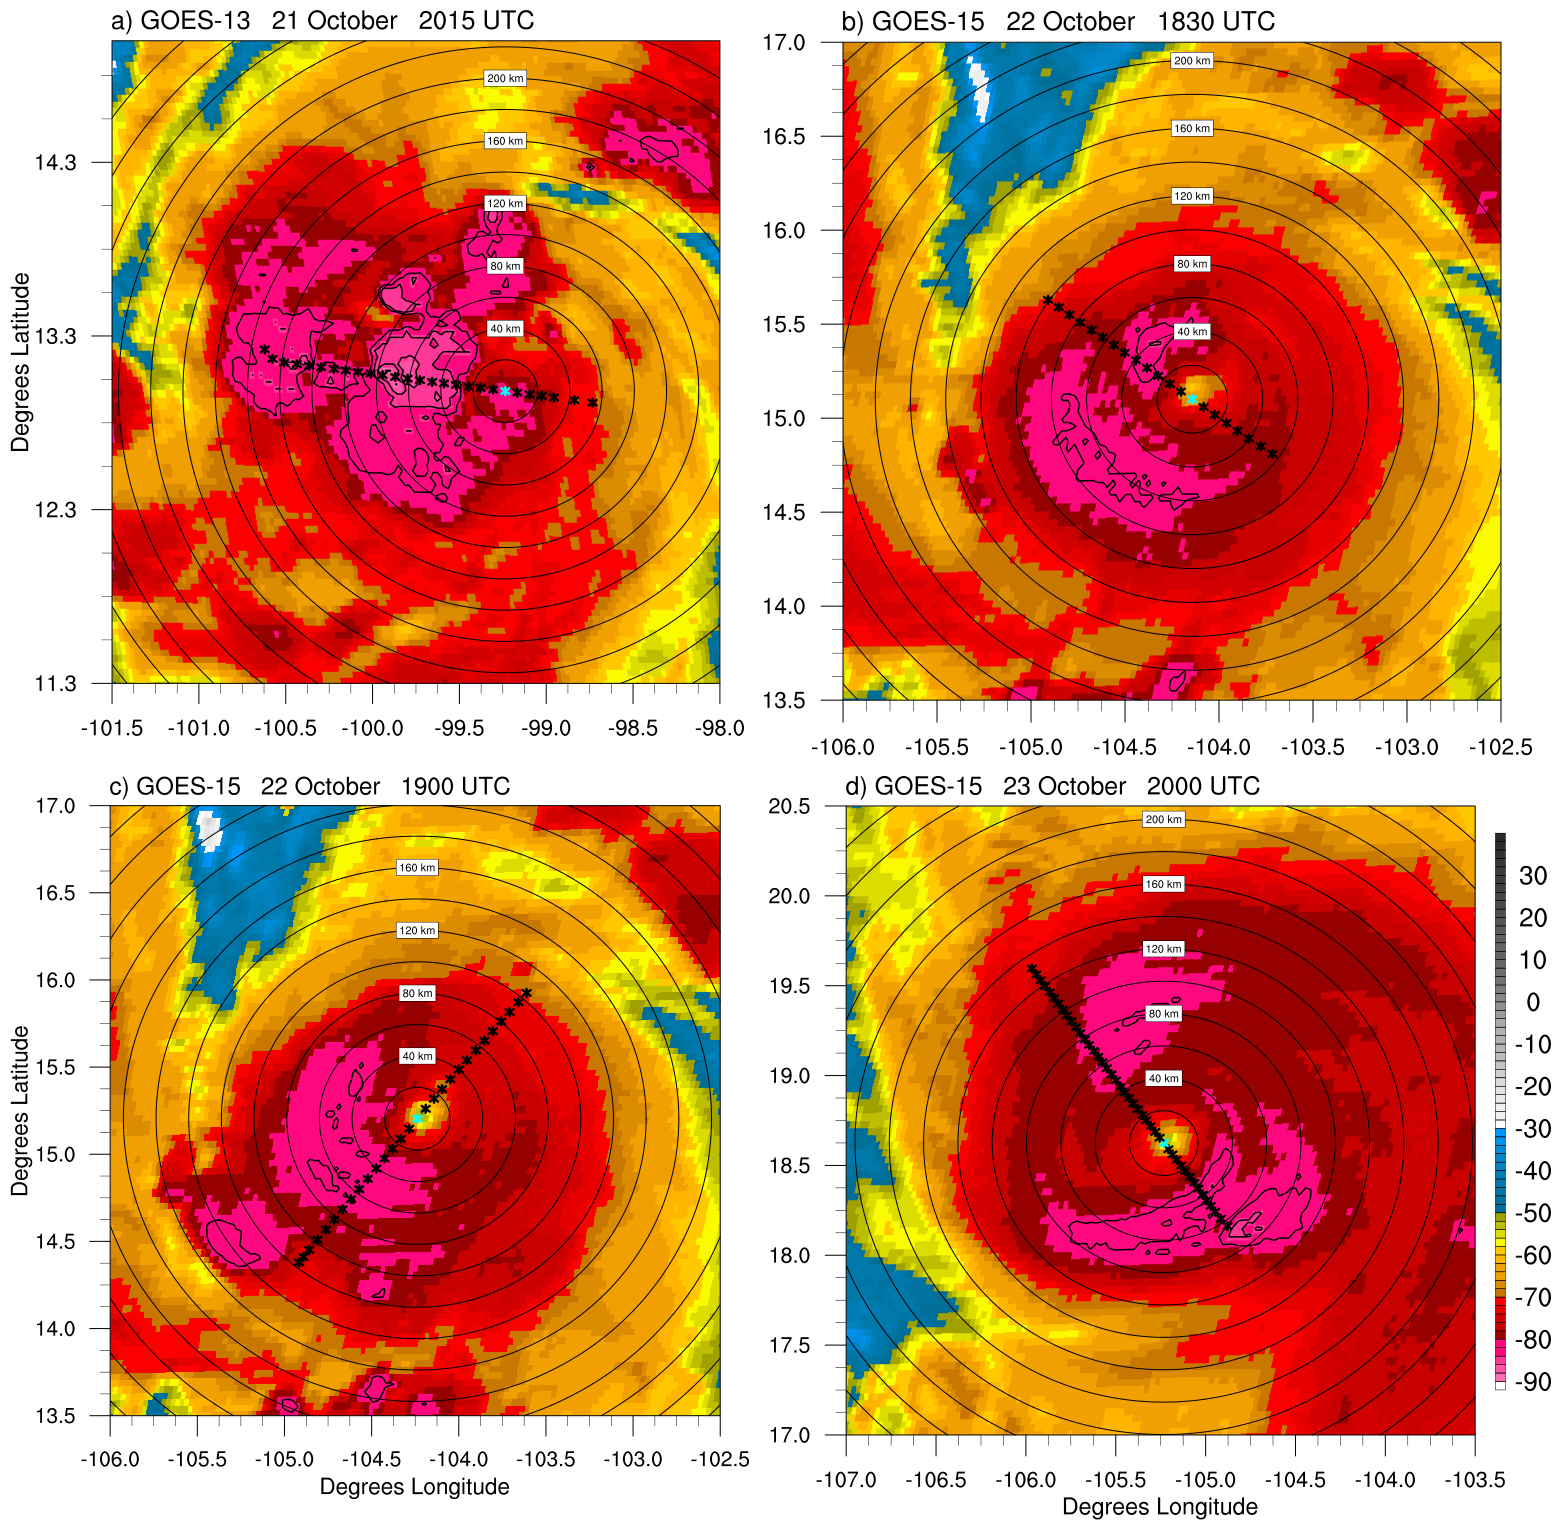
\includegraphics[width=39pc]{figures/fig01_patricia_ir.png}}
\caption{Infrared brightness temperature (\textdegree{}C) images of Tropical Storm Patricia at (a) 2015 UTC 21 Oct, and Hurricane Patricia at (b) 1830 UTC 22 Oct, (c) 1900 UTC 22 Oct, and (d) 2000 UTC 23 Oct 2015. Stars represent dropsonde deployment locations, with cyan stars marking the center location used for each cross section. Black contours delineate the coldest brightness temperatures, with a contour interval of 2\textdegree{}C starting at -82\textdegree{}C. The mean dropsonde spacing is (a) 7.9, (b) 7.8, (c) 8.0, and (d) 4.4 km for the four flight legs. Range rings are plotted every 20 km.}
\label{fig:patricia_ir}
\end{figure*}

%FIGURE 2%
\begin{figure*}[ht]
\centerline{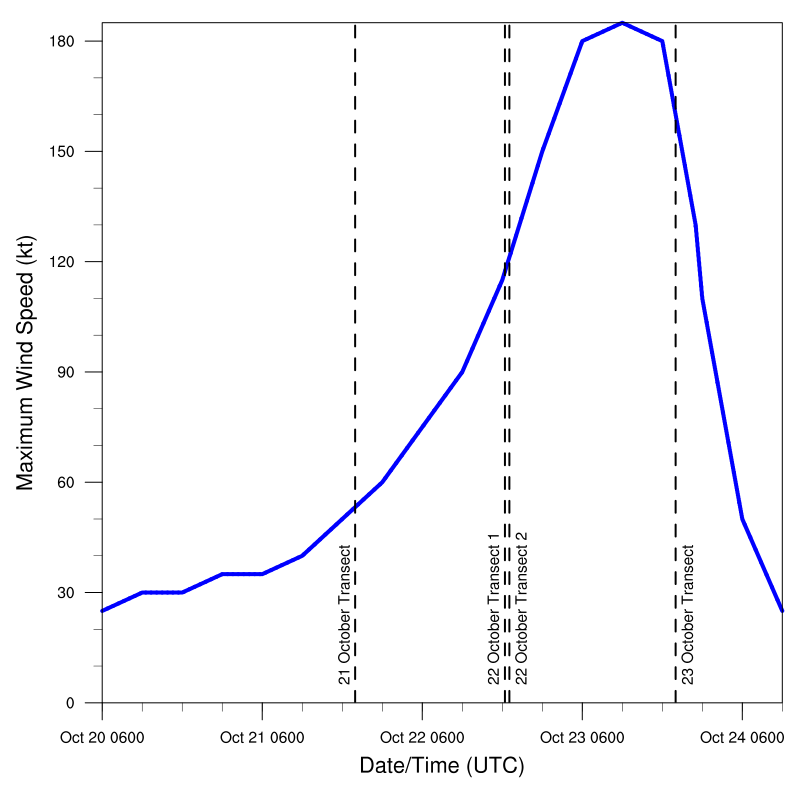
\includegraphics[width=39pc]{figures/fig02_patricia-intensity.png}}
\caption{The maximum wind speed (kt; blue line) throughout Patricia’s lifetime recorded in the National Hurricane Center best track \citep{Kimberlainetal2016}. Vertical lines indicate the times at which the WB-57 passed over the storm center during the four transects shown in Fig. \ref{fig:patricia_ir}.}
\label{fig:vmax}
\end{figure*}

%FIGURE 3%
\begin{figure*}[ht]
\centerline{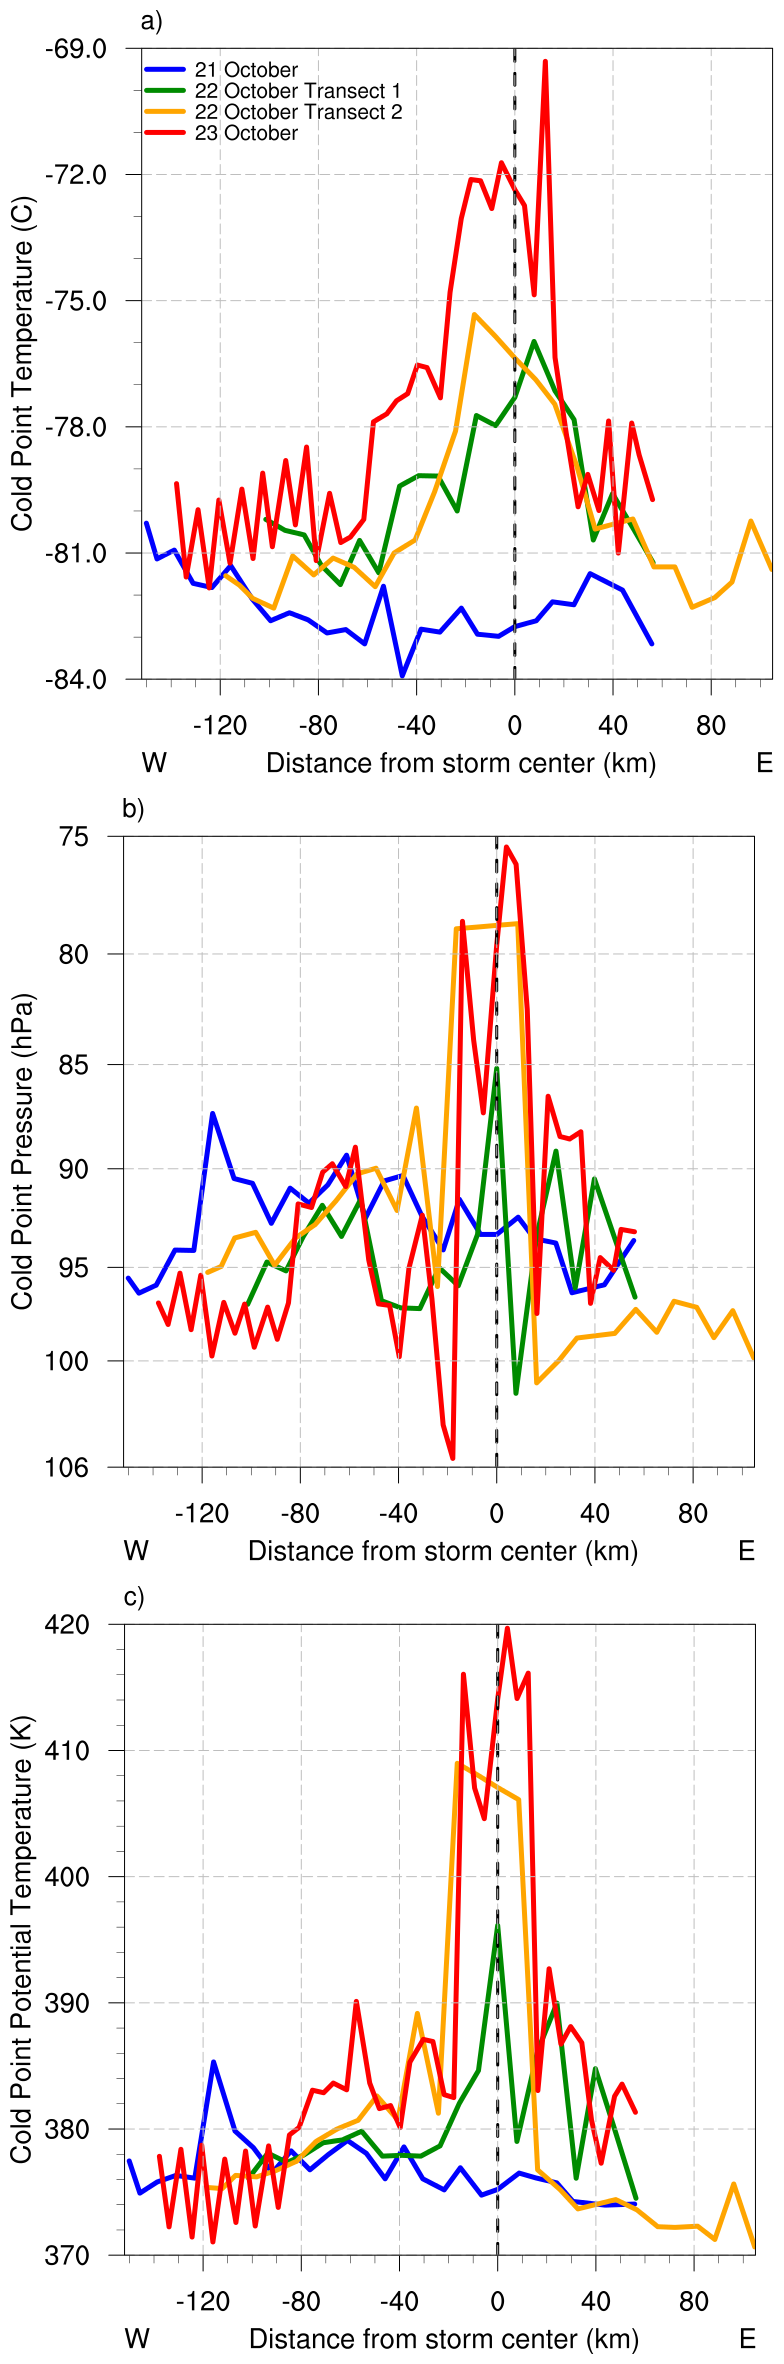
\includegraphics[width=16pc]{figures/fig03_cp_temp+theta+pres.png}}
\caption{(a) Temperature (\textdegree{}C), (b) pressure (hPa), and (c) potential temperature (K) at the cold-point tropopause for flights through the center of Tropical Storm Patricia at 1957 UTC 21 Oct (blue), and Hurricane Patricia at 1823 UTC 22 Oct (green), 1906} UTC 22 Oct (orange), and 2001 UTC 23 Oct (red) 2015. The vertical dashed lines represent the storm center. Compass directions are indicated by letters at each end of the cross section.
\label{fig:trop}
\end{figure*}

%FIGURE 4%
\begin{figure*}[ht]
\centerline{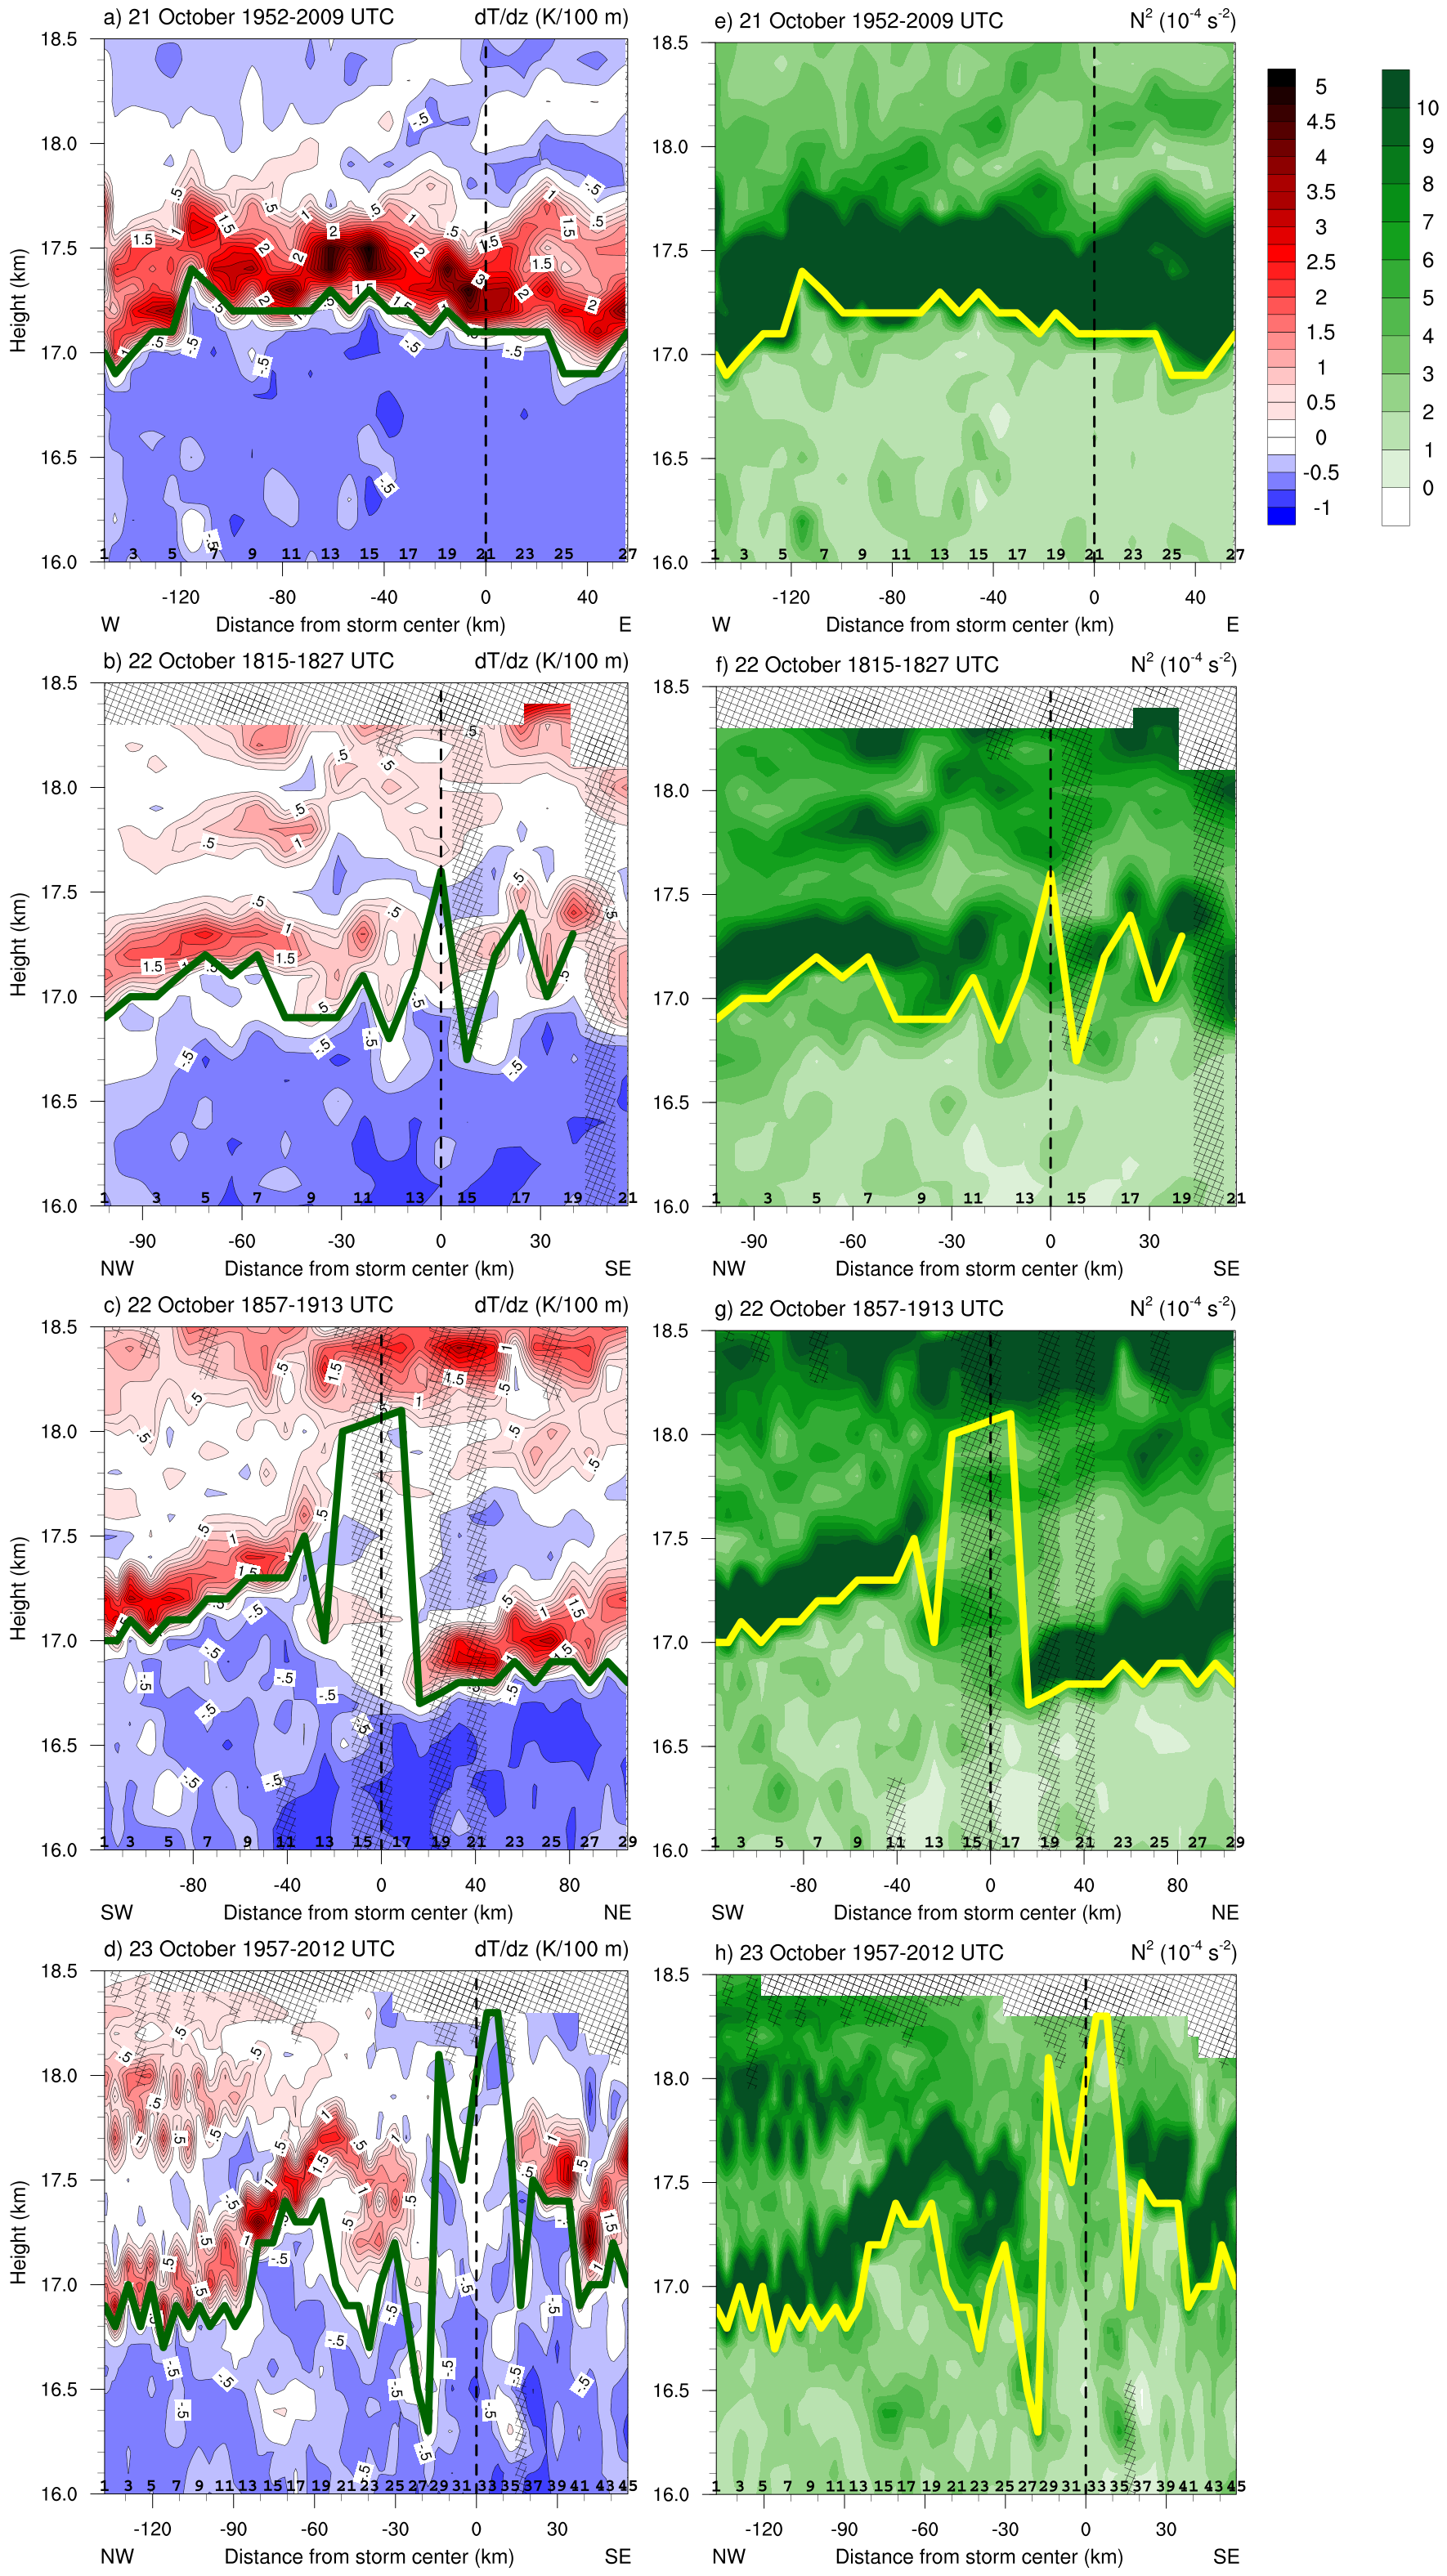
\includegraphics[width=24pc]{figures/fig04_dtdz+stab.png}}
\caption{(left) Vertical cross sections of $\Delta T/\Delta z$ [K (100 m)\textsuperscript{-1}; filled contours] and the cold-point tropopause height (green lines) along the transects shown in Fig. 1 on (a) 21; (b),(c) 22; and (d) 23 Oct 2015. Numbers along the bottom of each cross section represent the dropsonde deployment locations shown in Fig. 1 (only odd-numbered dropsondes are labeled here), with number 1 corresponding to the westernmost dropsonde. Compass directions are indicated by letters at each end of the cross sections. Dashed vertical lines mark the storm center and hatching indicates regions of missing values, where linear interpolation is performed in the radial direction. (right) Vertical cross sections of Brunt–Väisälä frequency squared (10\textsuperscript{-4} s\textsuperscript{-2}; filled contours) and cold-point tropopause height (yellow lines) on (e) 21; (f),(g) 22; and (h) 23 Oct 2015.}
\label{fig:stab}
\end{figure*}

%FIGURE 5%
\begin{figure*}[ht]
\centerline{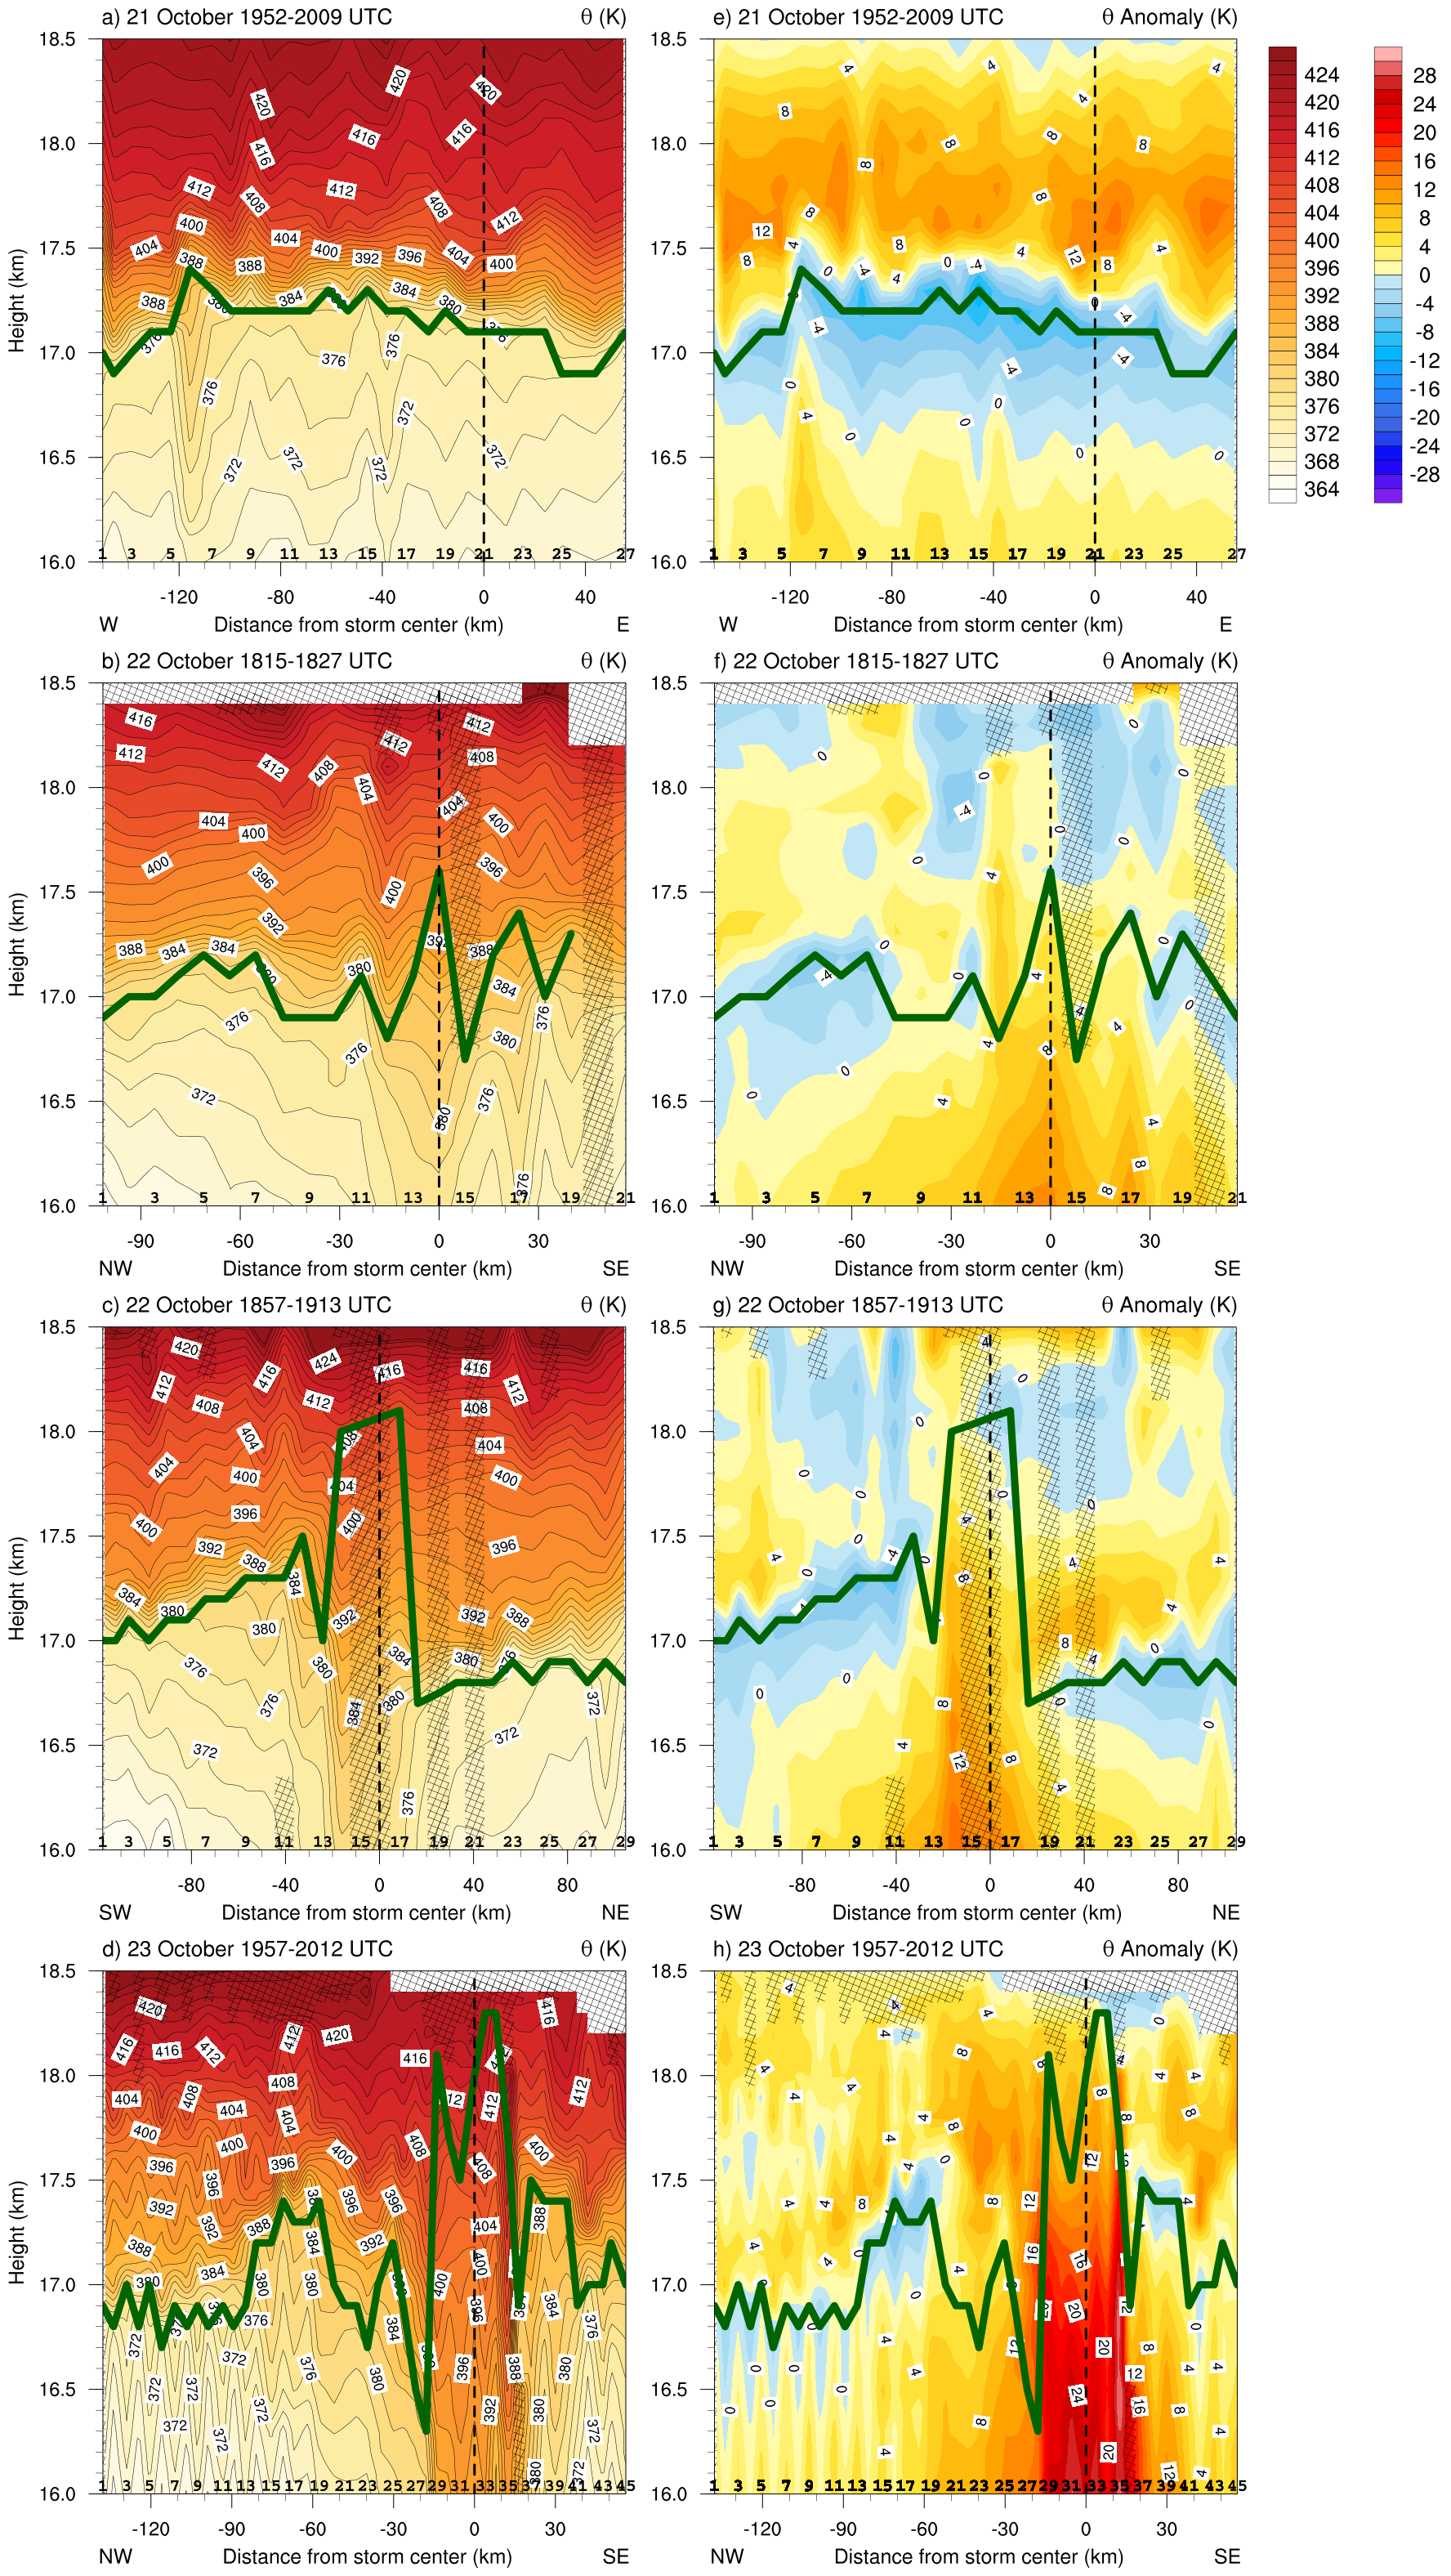
\includegraphics[width=24pc]{figures/fig05_theta+anomalies.png}}
\caption{(left) Vertical cross sections of potential temperature (\textdegree{}C; filled contours) and the cold-point tropopause height (green lines) along the transects shown in Fig. 1 on (a) 21; (b), (c) 22; and (d) 23 Oct 2015. Dropsonde locations, compass directions, and hatching as in Fig. \ref{fig:stab}. (right) Vertical cross sections of the potential temperature anomaly (\textdegree{}C) on (e) 21; (f),(g) 22; and (h) 23 Oct 2015.}
\label{fig:anomalies}
\end{figure*}

%FIGURE 6%
\begin{figure*}[ht]
\centerline{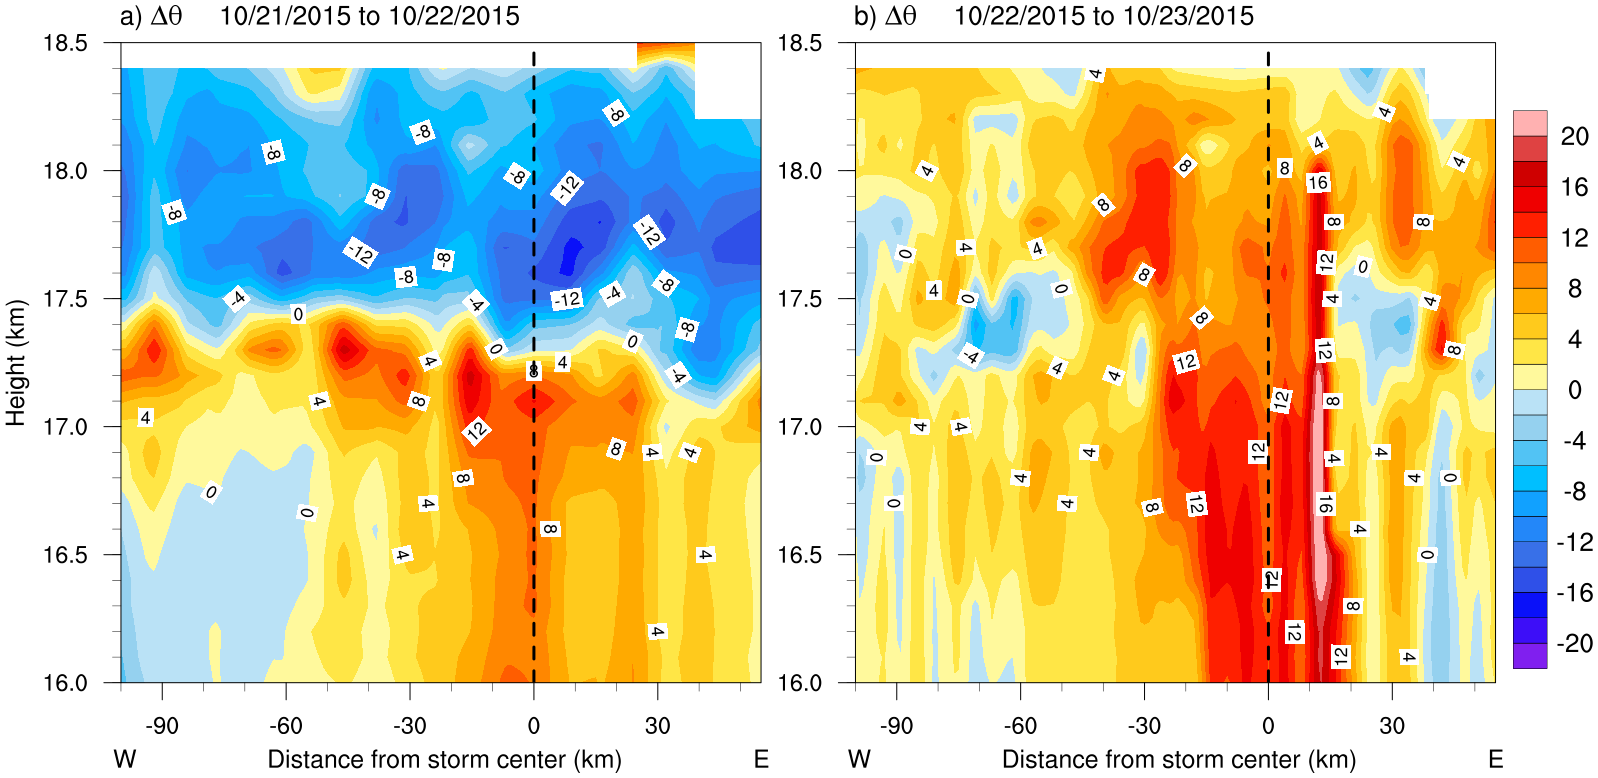
\includegraphics[width=39pc]{figures/fig06_deltatheta.png}}
\caption{Vertical cross sections of the potential temperature change (K day\textsuperscript{-1}) from (a) 21 to 22 Oct and (b) 22 to 23 Oct. These panels extend from the 100-km radius in Patricia’s western semicircle to 55 km in the eastern semicircle. The times separating the transects ($\Delta t$) were 22.45 h (21–22 Oct) and 25.63 h (22–23 Oct). To ease comparison between the two time periods, the potential temperature changes are scaled to 24 h by multiplying by ($24/\Delta t$).}
\label{fig:dtheta}
\end{figure*}

%FIGURE 7%
\begin{figure*}[ht]
\centerline{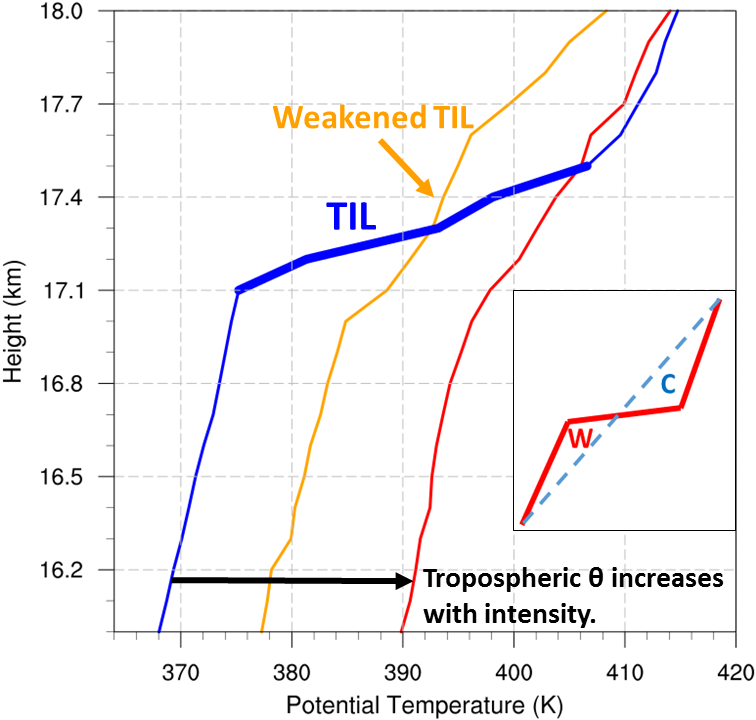
\includegraphics[width=33pc]{figures/fig07_schematic.png}}
\caption{Vertical profiles of potential temperature (K) between 16- and 18-km height for the soundings at Patricia’s storm center on 21 Oct (blue), 22 Oct (orange), and 23 Oct 2015 (red). The bolded segment of the blue line denotes the TIL on 21 Oct. (inset) A simplified schematic of mixing across a strongly stable layer, with the solid red line indicating the initial potential temperature profile and the dashed blue line representing the profile after a period of mixing; ‘‘W’’ and ‘‘C’’ represent regions of warming and cooling, respectively, after mixing.}
\label{fig:patricia-schematic}
\end{figure*}

%FIGURE 8%
\begin{figure*}[ht]
\centerline{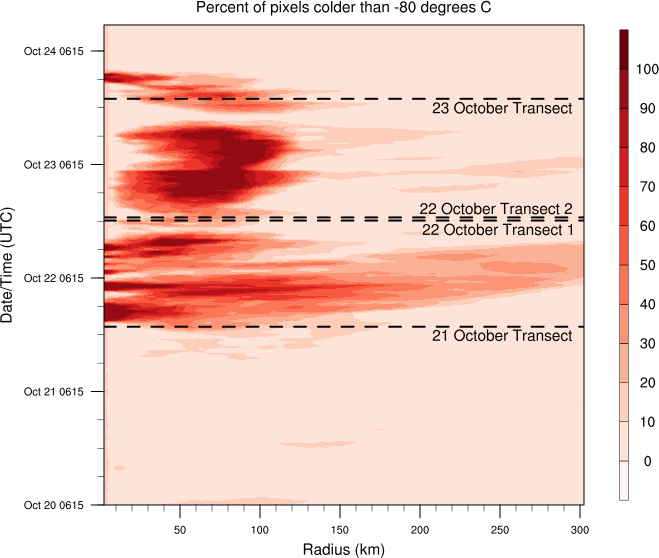
\includegraphics[width=39pc]{figures/fig08_hovmoller_tbpercent.png}}
\caption{Radius–time plot of the percent of infrared brightness temperature pixels colder than -80\textdegree{}C. The plot is constructed by counting the number of pixels colder than -80\textdegree{}C in a 5-km-wide radial bin, dividing by the total number of pixels in that bin, and multiplying by 100. This is performed every 5 km, extending from the storm center out to 300-km radius, for each GOES-13 image collected during Patricia’s lifetime (images are available every 30 min). Dashed black lines mark the times at which the WB-57 aircraft crossed over the storm center.}
\label{fig:hovmoller}
\end{figure*}

%FIGURE 9%
\begin{figure*}[ht]
\centerline{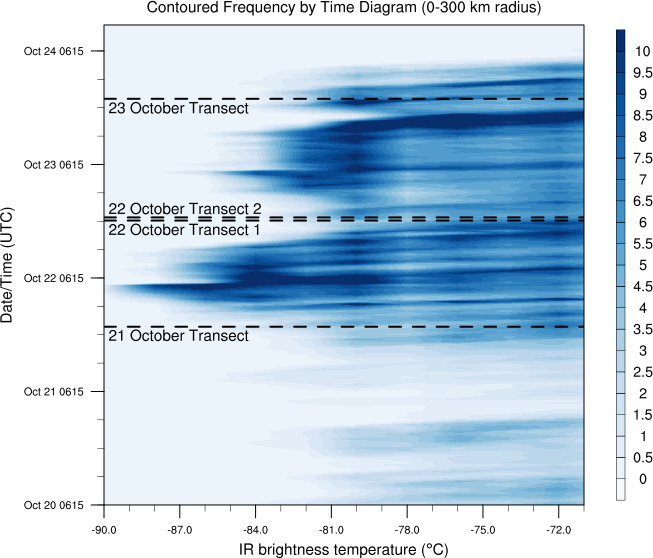
\includegraphics[width=39pc]{figures/fig09_CFTD.png}}
\caption{Contoured frequency by time diagram of infrared (IR) brightness temperature (\textdegree{}C) for all IR pixels within 300 km of the storm center observed by GOES-13 throughout Patricia’s lifetime. The plot is constructed by sampling the full distribution of IR brightness temperature within 300 km of the storm center and determining the percentage of pixels that fall into each IR brightness temperature bin (using 2-K-wide bins). Dashed black lines mark the times at which the WB-57 aircraft crossed over the
storm center.}
\label{fig:CFTD}
\end{figure*}

%FIGURE 10%
\begin{figure*}[ht]
\centerline{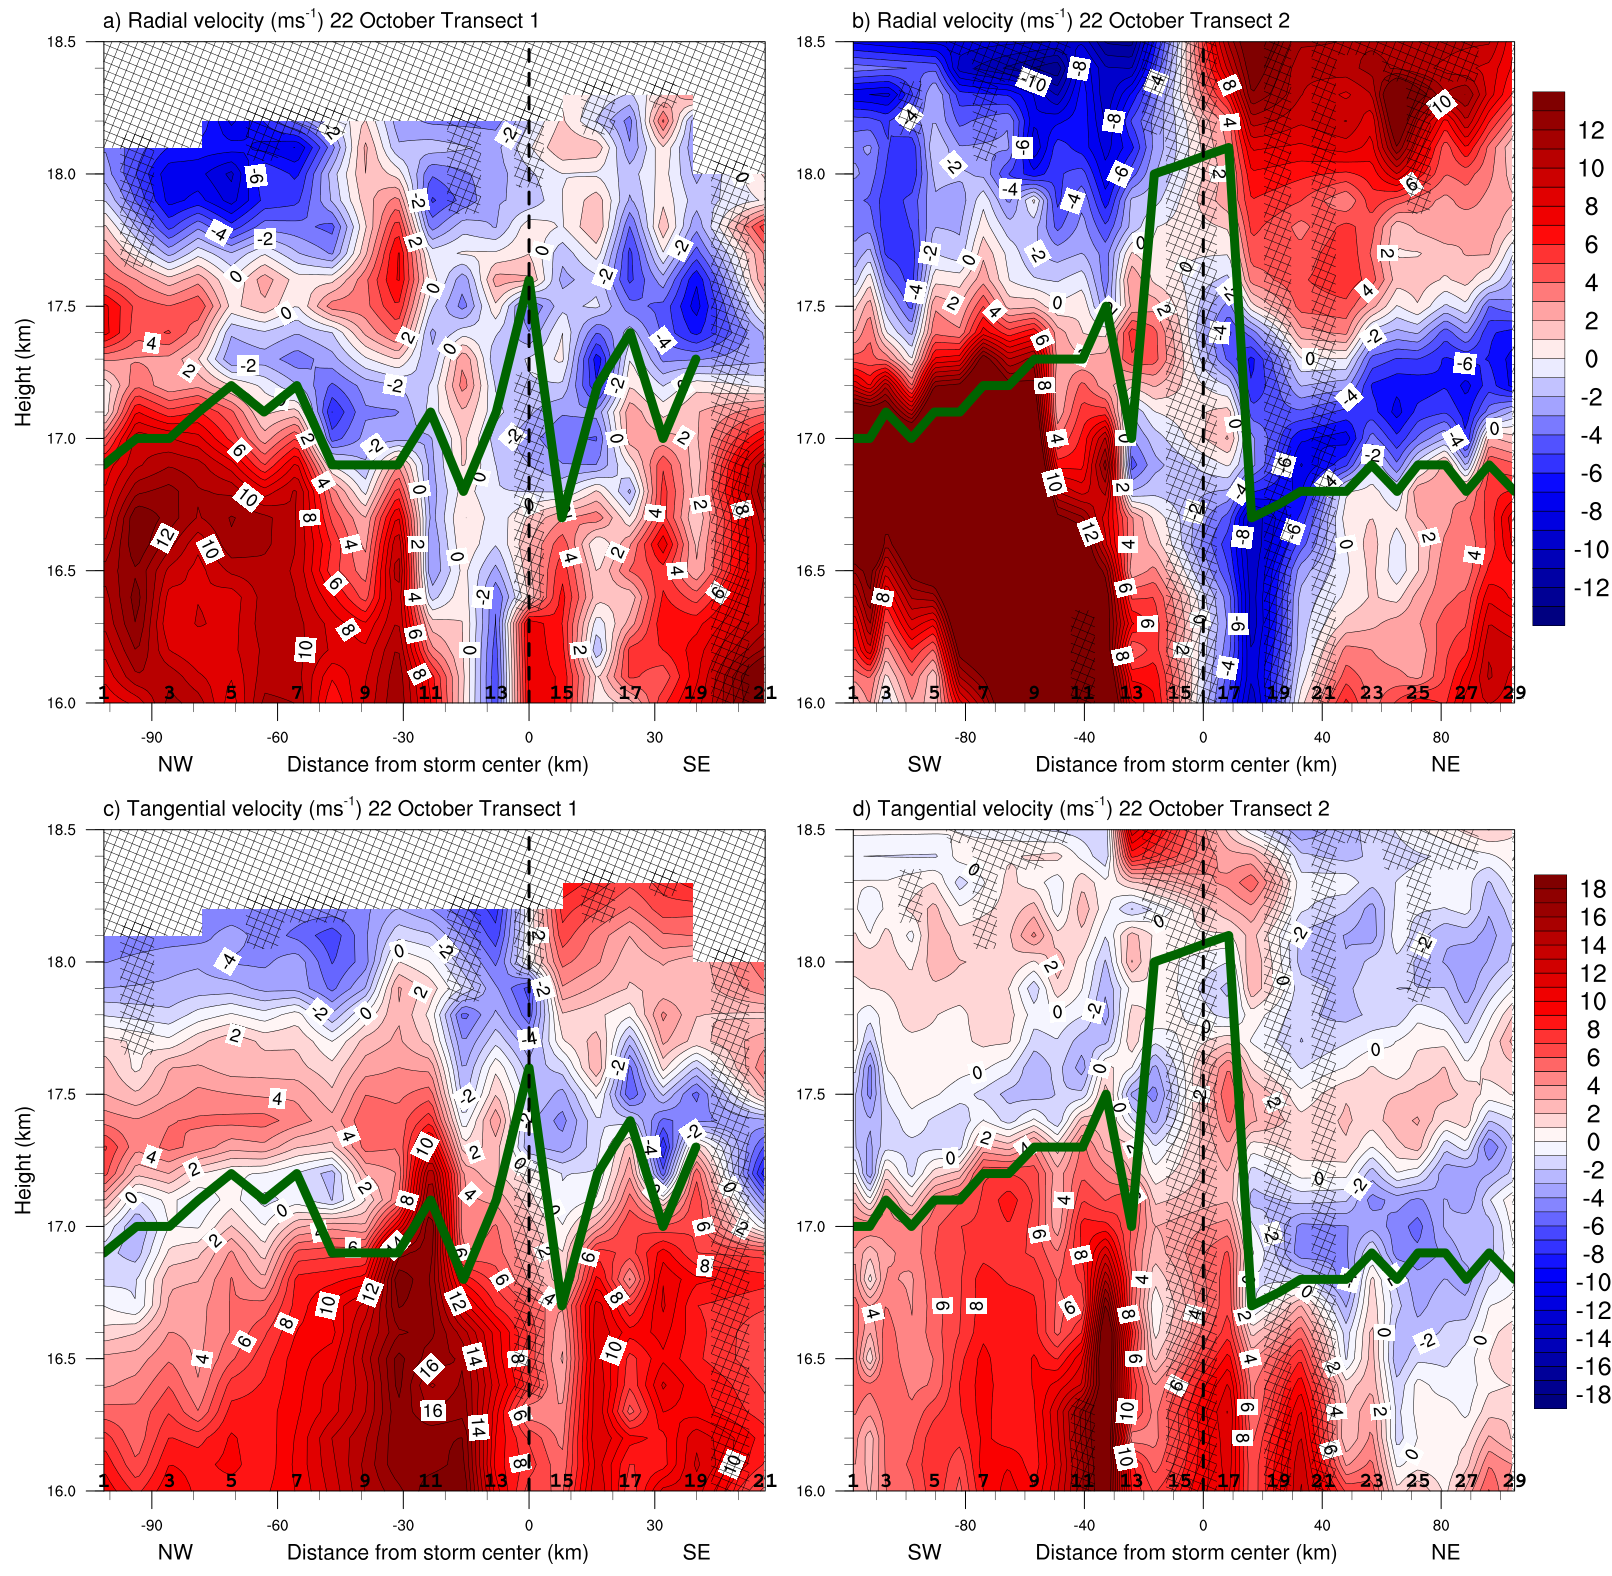
\includegraphics[width=39pc]{figures/fig10_velocities.png}}
\caption{Vertical cross sections of (a),(b) storm-relative radial and (c),(d) tangential velocity (m s\textsuperscript{-1}) and the cold-point tropopause height (green lines) in Hurricane Patricia for the two center-crossing transects on 22 Oct 2015. Dropsonde locations, compass directions, and vertical hatching as in Fig. \ref{fig:stab}.}
\label{fig:velocities}
\end{figure*}

%%%%%%%%%%%%%%%%%%%%%%%%%%%%%%%%%%%%%%%%%%%%%%%%%%%%%%%%%%%%%%%%%%% 
%                                                                 %
%                           CHAPTER 4                             %
%                                                                 %
%%%%%%%%%%%%%%%%%%%%%%%%%%%%%%%%%%%%%%%%%%%%%%%%%%%%%%%%%%%%%%%%%%% 
 
\chapter{Tropopause evolution in a rapidly intensifying tropical cyclone: A static stability budget analysis in an idealized, axisymmetric framework}
\label{chapter:modeling}
\resetfootnote %this command starts footnote numbering with 1 again.

\textbf{Submitted to Journal of the Atmospheric Sciences, in review.}

%---------------------------------------------------------------------------------------%
\section{Introduction}
%---------------------------------------------------------------------------------------%

The preceding chapter used dropsonde observations to document the tropopause-layer static stability evolution of Hurricane Patricia.
These observations alone, however, cannot explain the mechanisms that forced the static stability tendencies.
In this chapter, numerical simulations of an axisymmetric hurricane are conducted in an idealized, axisymmetric framework.
These simulations, which successfully reproduced the observed variability, provide some insight into the physical processes that might govern tropopause-layer static stability tendencies in TCs.

%---------------------------------------------------------------------------------------%
\section{Model setup}
%---------------------------------------------------------------------------------------%

The numerical simulations were performed using version 19.4 of Cloud Model 1 (CM1) described in \cite{BryanRotunno2009}.
The equations of motion were integrated on a 3000-km-wide, 30-km-deep axisymmetric grid with 1-km horizontal and 250-m vertical grid spacing.
The computations were performed on an \textit{f}-plane at 15\textdegree{N} latitude, over a sea surface with constant temperature of 30.5\textdegree C, which matches that observed near Hurricane Patricia (2015; \citeauthor{Kimberlainetal2016} \citeyear{Kimberlainetal2016}).
Horizontal turbulence was parameterized using the Smagorinsky scheme described in \citeauthor{BryanRotunno2009} (\citeyear{BryanRotunno2009}, pg. 1773), with a prescribed mixing length that varied linearly from 100 m at a surface pressure of 1015 hPa to 1000 m at a surface pressure of 900 hPa.
Vertical turbulence was parameterized using the formulation of \citeauthor{MarkowskiBryan2016} (\citeyear{MarkowskiBryan2016}, their Eq. 6), using an asymptotic vertical mixing length of 100 m.
A Rayleigh damping layer was applied outside of the 2900-km radius and above the 25-km level to prevent spurious gravity wave reflection at the model boundaries.
Microphysical processes were parameterized using the \cite{Thompson} scheme and radiative heating tendencies were computed every two minutes using the Rapid Radiative Transfer Model for GCMs (RRTMG) longwave and shortwave schemes \citep{Iacono}.
The initial temperature and humidity field was horizontally homogeneous and determined by averaging all Climate Forecast System Reanalysis (CFSR) grid points within 100 km of Patricia's center of circulation at 18 UTC 21 October 2015.
%A horizontally-homogeneous temperature and humidity field was initialized with a mean sounding computed using all dropsondes deployed during the TCI flight conducted within and around Tropical Storm Patricia on 21 October, 2015 (see \citeauthor{DoyleTCI} \citeyear{DoyleTCI} for details.)
%Above 19 km, where few TCI observations were available, the temperature profile was taken from the Climate Forecast System Reanalysis (CFSR) grid point nearest Patricia's storm center, valid at 18 UTC 21 October, 2015.
%Since relative humidity measurements were unreliable at temperatures below -40\textdegree C \citep{BellTCI}, relative humidity was set equal to 50\% above 11.5 km (the level above which temperature dropped below -40\textdegree C).
The vortex described in \citeauthor{RotunnoEmanuel} (\citeyear{RotunnoEmanuel}, their Eq. 37) was used to initialize the wind field, setting all parameters equal to the values used therein.

Although hurricanes simulated in an axisymmetric framework tend to be more intense than those observed in nature, the intensity evolution of this simulation matches reasonably well with that observed in Hurricane Patricia.
After an initial spin-up period of about 20 hours, the modeled storm (Fig.~\ref{fig:vmax+pmin}, blue lines) began an RI period that lasted approximately 30 hours.
After this RI, the storm continued to intensify more slowly until the maximum 10-m wind speed reached 89 m s\textsuperscript{-1} and the sea-level pressure reached its minimum of 846 hPa 81 hours into the simulation.
Hurricane Patricia (red stars) exhibited a similar intensity evolution prior to its landfall, with an RI period leading to a maximum 10-m wind speed of 95 m s\textsuperscript{-1} and a minimum sea-level pressure of 872 hPa.

%---------------------------------------------------------------------------------------%
\section{Budget computation}
%---------------------------------------------------------------------------------------%
The static stability can be expressed as the squared Brunt-V{\"a}is{\"a}l{\"a} frequency:
   \begin{equation} \label{eq:n2moist}
   N_m^2 = \frac{g}{T}\left(\frac{\partial T}{\partial z}+\Gamma_m\right)\left(1+\frac{T}{R_d/R_v+q_s}\frac{\partial q_s}{\partial T}\right)-\frac{g}{1+q_t}\frac{\partial q_t}{\partial z},
   \end{equation}
where $g$ is gravitational acceleration, $T$ is temperature, $R_d$ and $R_v$ are the gas constants of dry air and water vapor, respectively, $q_s$ is the saturation mixing ratio, $q_t$ is the total condensate mixing ratio, and $\Gamma_m$ is the moist-adiabatic lapse rate:
   \begin{equation} \label{eq:gamma_m}
   \Gamma_m = g(1+q_t)\left(\frac{1+L_vq_s/R_dT}{c_{pm}+L_v\partial q_s/\partial T}\right),
   \end {equation}
where $L_v$ is the latent heat of vaporization and $c_{pm}$ is the specific heat of moist air at constant pressure.
In the tropopause layer, $q_s$, ${\partial q_s}/{\partial T}$, and ${\partial q_t}/{\partial z}$ approach zero. In this limiting case, Eq. \ref{eq:n2moist} reduces to:
   \begin{equation} \label{eq:n2dry}
   N^2 = \frac{g}{\theta}\frac{\partial \theta}{\partial z},
   \end{equation}
where $\theta$ is the potential temperature.

To compute $N^2$, CM1 uses Eq. \ref{eq:n2moist} in saturated environments and Eq. \ref{eq:n2dry} in sub-saturated environments. For simplicity, however, only Eq. \ref{eq:n2dry} will be employed for the budget computations throughout the entire domain\footnote{The validity of this approximation will be substantiated later in this section.}.

Taking the time derivative of Eq. \ref{eq:n2dry} yields the static stability tendency:
   \begin{equation} \label{eq:dn2dt}
   \frac{\partial N^2}{\partial t} = \frac{g}{\theta}\frac{\partial}{\partial z}\frac{\partial \theta}{\partial t}-\frac{g}{\theta^2}\frac{\partial \theta}{\partial z}\frac{\partial \theta}{\partial t},
   \end{equation}
where the potential temperature tendency, $\partial \theta/\partial t$, can be written, following \cite{Bryan2017}:
   \begin{equation} \label{eq:dthetadt}
%   \frac{\partial \theta}{\partial t} = HADV+VADV+HTURB+VTURB+MP+RAD+DISS 
   \frac{\partial \theta}{\partial t} = -u\frac{\partial\theta}{\partial r}-w\frac{\partial \theta}{\partial z}+HTURB+VTURB+MP+RAD+DISS
   \end{equation}
Each term on the right-hand side of Eq.~\ref{eq:dthetadt} represents a $\theta$ budget variable, each of which is output directly by the model every minute.

The first term on the right-hand side of Eq. ~\ref{eq:dn2dt} is larger than the second term throughout most of the tropopause layer (not shown).
Consequently, the contribution of each of the terms in Eq.~\ref{eq:dthetadt} to the $N^2$ tendency can be interpreted in light of a vertical gradient of each term.
%Since the first term on the right-hand side of Eq.~\ref{eq:dn2dt} is larger than the second term throughout most of the tropopause layer (not shown), the contribution of each of the terms in Eq.~\ref{eq:dthetadt} to the $N^2$ tendency can be interpreted in light of a vertical gradient of each term.

Taking the vertical gradient of the first two terms on the right-hand side of Eq.~\ref{eq:dthetadt} yields the time tendency of the vertical $\theta$ gradient due to horizontal and vertical advection\footnote{These terms include the tendencies due to implicit diffusion in the fifth-order finite differencing scheme, which are separated from the advection terms in the CM1 version 19.4 budget output.}:

   \begin{equation} \label{eq:advtend}
   \left(\frac{\partial}{\partial t}\frac{\partial \theta}{\partial z}\right)_{adv} = -u\frac{\partial}{\partial r}\frac{\partial \theta}{\partial z}-w\frac{\partial}{\partial z}\frac{\partial \theta}{\partial z}-\frac{\partial u}{\partial z}\frac{\partial \theta}{\partial r}-\frac{\partial w}{\partial z}\frac{\partial \theta}{\partial z}.
   \end{equation}
The first two terms on the right-hand side of Eq.~\ref{eq:advtend} represent advection of static stability by the radial and vertical wind, respectively.
These terms act to rearrange the static stability field, but cannot strengthen or weaken static stability maxima or minima.
The third and fourth terms on the right-hand side of Eq.~\ref{eq:advtend} represent, respectively, the tilting of isentropes in the presence of vertical wind shear, and the stretching or squashing of isentropes by vertical gradients of vertical velocity.
Since these terms involve velocity gradients, they can act to strengthen or weaken static stability maxima or minima through differential advection.
Unless otherwise stated, any reference to "advection" in this paper indicates the sum of all of the terms in Eq.~\ref{eq:advtend}.

Returning to Eq.~\ref{eq:dthetadt}, HTURB and VTURB are the $\theta$ tendencies from the horizontal and vertical turbulence parameterizations, MP is the tendency from the microphysics scheme, RAD is the tendency from the radiation scheme, and DISS is the tendency due to turbulent dissipation.
This equation neglects Rayleigh damping, since the entire analysis domain lies outside of the regions where damping is applied.
Each term in Eq. \ref{eq:dthetadt} is substituted for ${\partial \theta}/{\partial t}$ in Eq. \ref{eq:dn2dt}, yielding the contribution of each budget term to the static stability tendency.
These terms are summed, yielding an instantaneous "budget change" in $N^2$ every minute.
The budget changes are then averaged over 24-hour periods and compared to the total model change in $N^2$ over that same time period, i.e.:
   \begin{equation} \label{eq:budgetchange}
   \Delta N^2_{budget} = \frac{1}{\delta t}\sum_{t=t_0}^{t_0+\delta t} \left.\frac{\partial N^2}{\partial t}\right\vert_t
   \end{equation}
   \begin{equation} \label{eq:modelchange}
   \Delta N^2_{model} = N^2_{t_0+\delta t}-N^2_{t_0}
   \end{equation}
   \begin{equation} \label{eq:residual}
   Residual = \Delta N^2_{model}-\Delta N^2_{budget}
   \end{equation}
where $t_0$ is an initial time and $\delta t$ is 24 hours.

Eqs. \ref{eq:budgetchange}-\ref{eq:residual} are plotted for three consecutive 24-hour periods in Fig.~\ref{fig:mod+bud+res}.
For this and all subsequent radial-vertical cross sections, a 1-2-1 smoother is applied once in the radial direction to eliminate $2\Delta r$ noise that appears in some of the raw model output and calculated fields.
      The left column of Fig.~\ref{fig:mod+bud+res} depicts the model changes computed using Eq.~\ref{eq:modelchange}, together with Eq.~\ref{eq:n2moist} in saturated environments and Eq. \ref{eq:n2dry} in subsaturated environments.
The center column depicts the budget changes computed using Eq. \ref{eq:budgetchange} together with Eq.~\ref{eq:n2dry} throughout the entire domain.
Thus, the left column includes the effect of moisture in the $N^2$ computations, whereas the center column neglects moisture.
The right column depicts the residuals, computed using Eq. \ref{eq:residual} (i.e. the left column minus the center column.)
In every 24-hour period, the budget changes are nearly identical to the model changes, which is reflected in the near-zero residuals in the right column.
This indicates that the budget accurately represents the model variability, which implies that the neglect of moisture in the budget computation introduces negligible error within the analysis domain\footnote{This is not the case in the lower- and mid-troposphere, where the residual actually exceeds the budget tendencies in many places, likely due to the neglect of moisture; thus we limit this analysis to the upper troposphere and lower stratosphere.}.

In the tropopause layer, some of the budget terms are small enough to be ignored.
To determine which of the budget terms are most important, a time series of the contribution of each of the budget terms in Eq. \ref{eq:dthetadt} to the tropopause-layer static stability tendency is plotted in Fig.~\ref{fig:avgbudterms}.
For this figure, each of the budget terms is computed using the method described in Section 3, except with 1-hour averaging intervals instead of 24-hour intervals.
The absolute values of these tendencies are then averaged over the radius-height domain of the plots shown in Fig.~\ref{fig:mod+bud+res} and plotted as a time series\footnote{It will be seeen in subsequent figures that each of the terms contributes both positively and negatively to the $N^2$ tendency within the analysis domain.
Thus, taking an average over the domain tends to wash out the positive and negative contributions.
To circumvent this problem, the absolute value of each of the terms is averaged.}.
Advection (Fig.~\ref{fig:avgbudterms}, red line) plays an important role in the mean tropopause-layer static stability tendency at all times, and vertical turbulence (Fig.~\ref{fig:avgbudterms}, blue line) and radiation (Fig.~\ref{fig:avgbudterms}, dark green line) also contribute significantly.
The remaining three processes - horizontal turbulence, microphysics, and dissipative heating -  are negligible everywhere outside of the eyewall, and do not play important roles in the mesoscale tropopause variability.

The preceding analysis indicates that, at all times, three budget terms dominate the tropopause-layer static stability tendency: advection, vertical turbulence, and radiation.
Variations in the magnitude and spatial structure of these terms drive the static stability changes depicted in Fig.~\ref{fig:mod+bud+res}; subsequent sections will focus on these variations and what causes them.

%---------------------------------------------------------------------------------------%
\section{Results}
%---------------------------------------------------------------------------------------%
 \subsection{Static stability evolution}

The average $N^2$ over the first day of the simulation (Fig.~\ref{fig:n2-24hr-avgs}a) indicates the presence of a weak $N^2$ maximum just above the cold-point tropopause.
Over the subsequent 24 hours, during the RI period, the $N^2$ within and above this layer decreased within the 25-km radius (Fig.~\ref{fig:n2-24hr-avgs}b).
This decreasing $N^2$ corresponded to an increase in the tropopause height within the developing eye, maximized at the storm center.
Outside of the eye, meanwhile, the tropopause height decreased over the eyewall region (25-60-km radius) and increased only slightly outside of the 60-km radius.
In this outer region, the $N^2$ maximum just above the tropopause strengthened during RI.
These trends continued as the storm's intensity leveled off in the 48-72-hour period (Fig.~\ref{fig:n2-24hr-avgs}c).
The tropopause height increased to nearly 21 km at the storm center and sloped sharply downward to 16.3 km on the inner edge of the eyewall, near the 30 km radius.
Static stability outside of the eye, meanwhile, continued to increase just above the cold-point tropopause.
This $N^2$ evolution closely follows that observed in Hurricane Patricia (2015; \citeauthor{DuranMolinari2018} \citeyear{DuranMolinari2018}, see their Fig. 4).
The mechanisms that led to these $N^2$ changes will be investigated in the subsequent sections.

 \subsection{Static stability budget analysis}

\paragraph{0-24 hours}\mbox{}\\
\indent The initial spin-up period was characterized by a steady increase of the maximum wind speed from 11 m s\textsuperscript{-1} to 22 m s\textsuperscript{-1} (Fig.~\ref{fig:vmax+pmin}a, blue line), an intensification rate that closely matched that of TC Patricia (Fig.~\ref{fig:vmax+pmin}a, red stars).
The weakening of the lower-stratospheric static stability maximum during this period is reflected in the total $N^2$ budget change over this time (Fig.~\ref{fig:stab-00-24}a).
The layer just above the cold-point tropopause was characterized by decreasing $N^2$ (purple shading), maximizing at the storm center.
At and immediately below the tropopause, meanwhile, $N^2$ increased during this time period (green shading).
Although these tendencies extended out to the 200-km radius, they were particularly pronounced at innermost radii.
A comparison of the contributions of advection (Fig.~\ref{fig:stab-00-24}b), vertical turbulence (Fig.~\ref{fig:stab-00-24}c), and radiation (Fig.~\ref{fig:stab-00-24}d) reveals that advection was the primary driver of the $N^2$ tendency during this period, acting to stabilize near and just below the tropopause and destabilize above.
Although vertical turbulence acted in opposition to advection (i.e. it acted to stabilize regions that advection acted to destabilize), the magnitude of the advective tendencies was larger, particularly at the innermost radii.
The sum of advection and vertical turbulence (Fig.~\ref{fig:stab-00-24}e) almost exactly replicated the static stability tendencies above the tropopause.
Radiative tendencies, meanwhile, (Fig.~\ref{fig:stab-00-24}d) acted to destabilize the layer below about 16 km and stabilize the layer between 16 and 17 km.
The sum of advection, vertical turbulence, and radiation (Fig.~\ref{fig:stab-00-24}f) reproduced the total change in $N^2$ almost exactly.

\paragraph{24-48 hours}\mbox{}\\
\indent During the RI period, the maximum wind speed increased from 22 m s\textsuperscript{-1} to 80 m s\textsuperscript{-1} (Fig.~\ref{fig:vmax+pmin}a).
Over this time, $N^2$ within the eye generally decreased above 16 km and increased below (Fig.~\ref{fig:stab-24-48}a), with the destabilization above 16 km maximizing near the level of the mean cold-point tropopause.
These tendencies at the innermost radii were driven almost entirely by advection (Fig.~\ref{fig:stab-24-48}b).
Vertical turbulence (Fig.~\ref{fig:stab-24-48}c) and radiation (Fig.~\ref{fig:stab-24-48}d) contributed negligibly to the static stability tendencies in this region.

Outside of the eye, the $N^2$ evolution exhibited alternating layers of positive and negative tendencies.
Near and above 18 km existed an upward-sloping region of decreasing $N^2$ that extended out to the 180-km radius.
In this region, neither vertical turbulence nor radiation exhibited negative $N^2$ tendencies; advection was the only forcing for this destabilization.
Immediately below this layer, just above the cold-point tropopause, was a region of increasing $N^2$ that sloped upward from 17 km near the 30-km radius to just below 18 km outside of the 100-km radius.
Advection and vertical turbulence both contributed to this positive $N^2$ tendency, with advection playing an important role below about 17.5 km and and turbulence playing an important role above.
The sum of advection and turbulence (Fig.~\ref{fig:stab-24-48}e) reveals two separate regions of increasing $N^2$ in the 17-18-km layer rather than one contiguous region.
The addition of radiation to these two terms, however, (Fig.~\ref{fig:stab-24-48}f) provides the link between these two regions, indicating that radiation also plays a role in strengthening the stable layer just above the tropopause.
In the 16-17-km layer, just below the cold-point tropopause, a horizontally-extensive layer of destabilization also was forced by a combination of advection, vertical turbulence, and radiation.
The sum of advection and vertical turbulence accounts for only a portion of the decreasing $N^2$ in this layer, and actually indicates forcing for stabilization near the 50-km radius and outside of the 130-km radius.
Radiative tendencies overcome this forcing for stabilization in both of these regions to produce the radially-extensive region of destabilization observed just below the tropopause.

The sum of advection, vertical turbulence, and radiation (Fig.~\ref{fig:stab-24-48}f) once again closely follows the observed $N^2$ variability, except in the eyewall region, where the neglect of latent heating and horizontal turbulence introduces some differences.

\paragraph{48-72 hours}\mbox{}\\
\indent After the storm's maximum wind speed leveled off near 80 m s\textsuperscript{-1} (Fig.~\ref{fig:vmax+pmin}a), the magnitude of the static stability tendencies within the eye decreased to near zero (Fig.~\ref{fig:stab-48-72}a).
Outside of the eye, however, $N^2$ continued to decrease in the layer immediately sorrounding the tropopause and increase just above.
The sum of advection and vertical turbulence (Fig.~\ref{fig:stab-48-72}e) indicates that these two processes account for most of the destabilization near the tropopause and some of the stabilization near the 18-km altitude.
Below the tropopause, however, these two terms provided strong forcing for stabilization that was not observed in the budget change (Fig.~\ref{fig:stab-48-72}a).
Radiation (Fig.~\ref{fig:stab-48-72}d), which generally forced stabilization above 17 km and destabilization below, balanced out this forcing for stabilization in the upper troposphere.
In the eyewall region (30-80-km radius), advection and vertical turbulence combined to force destabilization in the 17-18-km layer (Fig.~\ref{fig:stab-48-72}e), which was not observed in the budget change (Fig.~\ref{fig:stab-48-72}a).
Radiation provided strong forcing for stabilization, which outweighed this effect and produced net stabilization in a portion of this region.
Outside of the 80-km radius, both advection (Fig.~\ref{fig:stab-48-72}b) and vertical turbulence (Fig.~\ref{fig:stab-48-72}c) provided forcing for stabilization near and just above the 18-km level.
The sum of the two terms (Fig.~\ref{fig:stab-48-72}e) indicates increasing $N^2$ near the 18-km level everywhere outside of the 80-km radius, but this stabilization is slightly weaker in the 90-120-km radial band than the observed value.
The addition of radiation (Fig.~\ref{fig:stab-48-72}f) provided the extra forcing for stabilization required to account for the observed increase in $N^2$.
Outside of the 120-km radius, the region of radiative forcing for stabilization sloped downward, and the increase in $N^2$ observed near 18 km can be explained entirely by a combination of advection and vertical turbulence.

%---------------------------------------------------------------------------------------%
\section{Discussion}
%---------------------------------------------------------------------------------------%
  \subsection{The role of advection}

Advection played an important role in the tropopause-layer $N^2$ evolution at all stages of intensification, but for brevity, this section will focus only on the RI (24-48-hour) period.
To investigate the advective processes more closely, the individual contributions of horizontal and vertical advection during the RI period are shown in Fig.~\ref{fig:adv-24-48}, along with the corresponding time-mean radial and vertical velocities and $\theta$.
The $N^2$ tendencies due to the two advective components (Fig.~\ref{fig:adv-24-48}a,b) exhibited strong cancellation, consistent with flow that was nearly isentropic.
There existed, however, a large region near the tropopause in which the total advective tendency was nonzero (Fig.~\ref{fig:stab-24-48}b).
These nonzero tendencies were related to the development of the TC's secondary circulation as the storm intensified.

%The eye was characterized by stabilization below 16 km and destabilization in the 16-17-km and 18-19-km layers.
%Comparing Fig.~\ref{fig:stab-24-48}b to \ref{fig:adv-24-48}a,b reveals that the stabilization below 16 km in the eye was forced by vertical advection, as was the region of destabilization in the 18-19-km layer.
%Meanwhile, the destabilization that occurred in the 16-17-km layer was forced by a combination and radial and vertial advection.

%Outside of the eye, the layer below about 15.5 km was dominated by stabilization.
%Outside of the 50-km radius, horizontal advection provided the forcing for this stabilization, while inside of the 50-km radius, vertical advection was responsible.
%Above this layer existed a layer of destabilization near the 16-km level, which was forced by horizontal advection.


%Some insight can be gained by considering the time tendency of the vertical $\theta$ gradient due to advection:
%   \begin{equation} \label{eq:advtend}
%   \left(\frac{\partial}{\partial t}\frac{\partial \theta}{\partial z}\right)_{adv} = -u\frac{\partial}{\partial r}\frac{\partial \theta}{\partial z}-w\frac{\partial}{\partial z}\frac{\partial \theta}{\partial z}-\frac{\partial u}{\partial z}\frac{\partial \theta}{\partial r}-\frac{\partial w}{\partial z}\frac{\partial \theta}{\partial z}.
%   \end{equation}

%The first two terms on the right-hand side of Eq. \ref{eq:advtend} represent advection of static stability by the radial and vertical wind, respectively.
%These terms cannot create a maximum or a minimum; they only act to rearrange the static stability field.
%Since the goal of this analysis is to understand the processes responsible for the creation of maxima and minima in $N^2$, these two terms will not be examined.
%The third and fourth terms represent, respectively, the tilting of isentropes in the presence of vertical wind shear, and the spreading or compaction of isentropes through divergence of the vertical wind.
%Since these terms involve gradients of velocities, they can create or eliminate local maxima or minima in static stability.% This section will focus on these two terms.

%  \paragraph{0-24 hours}
%During the first day of the simulation, horizontal advection (Fig.~\ref{fig:adv-00-24}a) generally forced a decrease in $N^2$ below 17 km and an increase in $N^2$ above.
%The mean radial velocity during this period (Fig.~\ref{fig:adv-00-24}c) reveals a region of outflow at and below 17 km and near-zero radial velocity above, with a layer of strong vertical wind shear straddling the tropopause.
%The slight downward slope with radius of the $\theta$ surfaces near the tropopause (i.e. $\partial\theta/\partial r > 0$), together with strong vertical wind shear ($\partial u/\partial z < 0$) in this layer, acts to force an increase in the vertical gradient of $\theta$ above 17 km through the third term on the right-hand side of Eq. \ref{eq:advtend}.
%This negative $\theta$ tendency must decrease with height within the region of strong vertical wind shear and approach zero as the radial velocity diminishes to zero near 17 km.
%These tendencies thus yielded an increase in the vertical gradient of $\theta$ above 17 km, which implies an increase in $N^2$, as was seen in Fig.~\ref{fig:adv-00-24}a.
%Note that although the radial gradient of $\theta$ was stronger in the 15-16-km layer than it was closer to the tropopause, the vertical shear of the radial wind was much smaller there, yielding a smaller $N^2$ tendency due to horizontal advection.
%
%Notably, there existed strong $N^2$ tendencies due to horizontal advection inside of the 30-km radius even though the mean radial velocity in that region was near zero.
%Close examination of the radial velocity at each output time step reveals the presence of inward-propagating waves in the lower stratosphere.
%These waves amplified upon reaching r=0 and forced strong but highly transient $\theta$ tendencies due to advective processes.
%Thus, although the radial velocity perturbations associated with these waves averaged out to zero, the non-linear effect of these waves on the $N^2$ field remained.
%
%The $N^2$ tendencies forced by horizontal advection were completely canceled out by vertical advective tendencies (\ref{fig:adv-00-24}b).
%As was seen in Fig.~\ref{fig:stab-00-24}b, the sum of the two terms yielded a layer of increasing $N^2$ below 17 km and decreasing $N^2$ above, meaning that vertical advective processes dominated the $N^2$ tendency during the initial spin-up period.
%Most of the upper troposphere contained mean ascent during this time, with the magnitude of the ascent decreasing with height.
%This decrease in upward motion with height forces a convergence of isentropic surfaces, which implies a positive $N^2$ tendency in this region, as was observed in Fig.~\ref{fig:adv-00-24}b.
%Some weak descent at and just above the tropopause, meanwhile, forces a slight divergence of isentropes in the 17-18-km layer and a concomitant decrease in $N^2$.
%Surprisingly, the 0-20-km radius was characterized by mean ascent, even up to the 21-km level.
%Inward-propagating waves, upon reaching r=0, induced dipoles of strong upward and downward vertical motion.
%For reasons that remain unclear, the regions of ascent tended to last longer than the regions of subsidence induced by these waves, which is responsible for the dominance of ascent in the mean.
%In this region of mean ascent, changes in the vertical gradint of mean vertical velocity are responsible for alternating regions of positive and negative $N^2$ tendencies.
%
%HOVMOLLER OF w IN THE LOWER STRATOSPHERE??

%   \paragraph{RI period: 24-48 hours}
During the RI period, strong radial and vertical circulations developed near the tropopause (Fig.~\ref{fig:adv-24-48}c,d), which forced high-magnitude $N^2$ tendencies due to advection (Fig.~\ref{fig:adv-24-48}a,b).
A layer of strong outflow formed at and below the tropopause during this period, with the outflow maximum (dashed cyan line) curving from the 14-km level at the 50-km radius to just below the 16-km level outside of the 80-km radius (Fig.~\ref{fig:adv-24-48}c).
%The cyan line, by definition, represents the level at which the vertical gradient of radial velocity switched signs, with $\partial u/\partial z>0$ below the line and $\partial u/\partial z<0$ above.
Notably, the $N^2$ tendency due to horizontal advection (Fig.~\ref{fig:adv-24-48}a) tended to switch signs at this line, with stabilization below the outflow maximum and destabilization above.
%This suggests that vertical wind shear above and below the outflow maximum played an important role in the $N^2$ tendency during this time.
%Examination of the third term on the right-hand side of Eq. \ref{eq:advtend} suggests that tilting of isentropes within these shear layers contributed to the strong $N^2$ tendencies that flanked the outflow maximum.
This is consistent with the outflow layer carrying air with increasingly large $\theta$ from the eyewall to large radii as the storm intensified.
This increase in $\theta$ maximized near the outflow maximum, which acted to decrease $\partial \theta/\partial z$ above the outflow maximum and increase it below.
%Outside of the eye and eyewall, isentropes generally sloped upward with radius.
%Vertical wind shear acting on these upward-sloping isentropes should act to tilt them into the vertical above the outflow maximum, thereby decreasing $\partial \theta/\partial z$, and tilt them to be more horizontal below the outflow maximum, thereby increasing $\partial \theta/\partial z$.
This mechanism is the same as that discussed in \cite{TrierSharman2009}, in which vertical wind shear in the outflow layer of a mesoscale convective system modified the upper-tropospheric static stability through differential advection of isentropes.
%Thus, wherever $\partial u/\partial z>0$, the tilting term must force an increase in $N^2$, and wherever $\partial u/\partial z<0$, the tilting term must force a decrease in $N^2$, which is precisely the structure seen in Fig.~\ref{fig:adv-24-48}a.

%Advection of $N^2$ by the radial wind (first term on the right-hand side of Eq. \ref{eq:advtend}) also acted within the outflow jet.
%For example, horizontal advection provided forcing for destabilization at the 16-km level almost everywhere inside of the 140-km radius.
%Outside of this radius near 16 km, however, existed a region of forcing for stabilization.
%This switch in signs was a consequence of a reversal of the radial graident of mean $N^2$ near the 140-km radius (Fig.~\ref{fig:n2-24hr-avgs}b).
%Inside of that radius, $(\partial/\partial r)(\partial \theta/\partial z) > 0$ and $u > 0$, which corresponds to forcing for destabilization in Eq. \ref{eq:advtend}; outside of that radius $(\partial/\partial r)(\partial \theta/\partial z) < 0$ and $u > 0$, which corresponds to forcing for stabilization.
%
%The relative imporance of the first and third terms on the right-hand side of Eq. \ref{eq:advtend} is difficult to ascertain, but the structure of the mean radial velocity, $\theta$, and $N^2$ fields suggests that both terms are contributing within the outflow layer.

Meanwhile in the lower stratosphere, a thin layer of 2-4 m s\textsuperscript{-1} inflow developed a few hundred meters above the tropopause, similar to that which was observed in Hurricane Patricia (2015; \citeauthor{DuranMolinari2018} \citeyear{DuranMolinari2018}) and in previous modeling studies (e.g. \citeauthor{OhnoSatoh2015} \citeyear{OhnoSatoh2015}; \citeauthor{Kieuetal2016} \citeyear{Kieuetal2016}).
Since the isentropes in this layer sloped slightly upward with radius (i.e. $\partial \theta/\partial r < 0$), this inflow acted to import lower $\theta$ air from outer radii to inner radii.
%There also existed strong radial gradients of mean $N^2$ in this layer during this time (Fig.~\ref{fig:n2-24hr-avgs}b), so the inflow layer must have acted to rearrange $N^2$.
%This rearrangement could not have been responsible for the overall increase in $N^2$ during this period, however.
%If horizontal advection contributed to the strengthening stable layer just above the tropopause, it must have been through the tilting term.
%The inflow maximum near the 18-km level represents the level at which the sign of $\partial u/\partial z$ reverses, with $\partial u/\partial z < 0$ below and $\partial u/\partial z > 0$ above.
%The third term on the right-hand side of Eq. \ref{eq:advtend} shows that the tilting of isentropes should act to destabilize the layer below the inflow maximum and stabilize the layer above, which is precisely what was observed outside of the 80-km radius in Fig.~\ref{fig:adv-24-48}a.
Since the negative $\theta$ tendencies maximized at the level of maximum inflow, the layer below the inflow maximum destabilized and the layer above stabilized (Fig.~\ref{fig:adv-24-48}a).

Curiously, horizontal advection contributed to the $N^2$ tendency everywhere within the eye, even though the mean radial velocity there was near zero.
Close examination of the model output revealed that these tendencies were forced by advective processes associated with inward-propagating waves.
%Close examination of the model output revealed that this mean ascent was forced by the interaction of inward-propagating waves with the boundary at r=0.
Although the radial velocity perturbations induced by these waves averaged out to zero, the advective tendencies forced by the radial velocity perturbations did not.
Additionally, when these waves reached r=0, a dipole of vertical velocity resulted, with ascent above and descent below.
For reasons that remain unclear, the regions of ascent were more persistent than the regions of descent, which resulted in the mean ascent observed near r=0 above 17 km in Fig.~\ref{fig:adv-24-48}d.

Vertical advection also played an important role in the tropopause-layer static stability evolution.
Within the eye, subsidence dominated below 17 km, while mean ascent existed near the storm center above 17 km.
Although the magnitude of the subsidence was larger at lower altitudes, $\partial \theta/\partial z$ was smaller there.
Because $\partial \theta/\partial z$ was smaller, the subsidence at lower levels could not accomplish as much warming as the subsidence at higher levels in the eye, consistent with the results of \cite{SternZhang2013}.
As a result, vertical advection within the eye stabilized the layer below 16 km during RI.

Outside of the 27-km radius, ascent dominated the troposphere, while a 1-1.5-km-deep layer of descent existed immediately above the tropopause.
These regions of ascent and descent converged just above the tropopause; this convergence acted to compact the isentropes in this layer and increase the static stability.
Above the lower-stratospheric subsidence maximum, meanwhile, vertical advection decreased $N^2$.
Below the tropopause, differential vertical advection increased $N^2$ within the eyewall region and also at larger radii above the vertical velocity maximum at larger radii.
Outside of the eyewall and below the vertical velocity maximum, meanwhile, differential vertical advection acted to decrease $N^2$.

Comparing the $N^2$ tendencies forced by horizontal (Fig.~\ref{fig:adv-24-48}a) and vertical (Fig.~\ref{fig:adv-24-48}b) advection to the total advective tendency seen in Fig.~\ref{fig:stab-24-48}b reveals that horizontal advective tendencies dominated the troposphere, while vertical advective tendencies dominated the layer near and above the tropopause.
Thus, tilting of isentropes in the vicinity of the upper-tropospheric outflow maximum appears to be the most important advective process governing the $N^2$ tendency in the troposphere, whereas convergence of vertical velocity appears to be the most important advective process near the tropopause.


  \subsection{The role of radiation}
During the initial spin-up period (0-24 hours; Fig.~\ref{fig:qi+radten}a), convection was not deep enough to deposit large quantities of ice near the tropopause and create a persistent cirrus canopy.
Due to the lack of ice particles, the radiative heating tendencies during this period (Fig.~\ref{fig:qi+radten}b) were relatively small and confined to the region above a few particularly strong, although transient, convective towers.
During RI (24-48 hours), the eyewall updraft strengthened and a radially-extensive cirrus canopy developed near the tropopause (Fig.~\ref{fig:qi+radten}c).
The enhanced vertical gradient of ice mixing ratio at the top of the cirrus canopy induced strong diurnal-mean radiative cooling near the tropopause (Fig.~\ref{fig:qi+radten}d).
This cooling exceeded 0.6 K h\textsuperscript{-1} (14.4 K day\textsuperscript{-1}) in some places and sloped downward from the lower stratosphere into the upper troposphere, following the top of the cirrus canopy.
A small radiative warming maximum also appeared outside of the 140-km radius below this region of cooling.
These results broadly agree with those of \citeauthor{Buetal2014} (\citeyear{Buetal2014}; see their Fig. 11a), whose CM1 simulations produced a 0.3 K h\textsuperscript{-1} diurnally-averaged radiative cooling at the top of the cirrus canopy and radiative warming within the cloud that maximized near the 200-km radius.
This broad region of radiative cooling acted to destabilize the layer below the cooling maximum and stabilize the layer above, which can be seen in Fig.~\ref{fig:stab-24-48}d.
The small area of net radiative heating outside of the 140-km radius enhanced the destabilization above 16 km in this region and produced a thin layer of stabilization in the 15-16-km layer.

After the TC's RI period completed (48-72 hours), strong radiative cooling remained near the tropopause at inner radii (Fig.~\ref{fig:qi+radten}f), sloping downward with the top of the cirrus canopy to below the tropopause at outer radii.
Cooling rates exceeded 1 K h\textsuperscript{-1} (24 K day\textsuperscript{-1}) just above the tropopause between the 30- and 70-km radii.
This value is more than three times the maximum cooling rate of 0.3 K h\textsuperscript{-1} observed by \cite{Buetal2014}, a difference that is a consequence of their larger vertical grid spacing compared to that used here, along with a contribution from differing radiation schemes.
%\cite{Buetal2014} employed the NASA-Goddard radiation scheme in their CM1 simulations, whereas RRTMG is used in the present paper.
To compare our results to theirs, we ran a simulation identical to that described in Section 2, except using the NASA-Goddard radiation scheme and 625-m vertical grid spacing, to match those of \cite{Buetal2014}.
This simulation produced a maximum 24-hour-average radiative cooling rate of 0.3 K h\textsuperscript{-1}, which agrees with that shown in \cite{Buetal2014}.
Another simulation using 625-m vertical grid spacing and RRTMG radiation produced 24-hour-average cooling rates of up to 0.6 K h\textsuperscript{-1}.
This suggests that vertical grid spacing smaller than 625 m is necessary to resolve properly the radiative cooling at the top of the cirrus canopy, and that the results can be quite sensitive to the radiation scheme used.

Meanwhile below the tropopause, time-mean radiative warming spread from 30- to 160-km radius within the cirrus canopy.
The existence of radiative cooling overlying radiative warming in this region led to radiatively-forced destabilization at and below the tropopause, as was observed in Fig.~\ref{fig:stab-48-72}d.
Beneath the warming layer existed a region of forcing for stabilization, while a much stronger region of forcing for stabilization existed in the lower stratosphere, above the cooling maximum.

The results herein suggest that, after the cirrus canopy developed, radiative heating tendencies considerably destabilized the upper troposphere and stabilized the lower stratosphere.

  \subsection{The role of turbulent mixing}

%An interesting result of the budget analysis was that turbulent mixing acted to increase static stability in some regions of the storm.
%Although vertical turbulence always acts to eliminate vertical gradients of $\theta$, this adjustment toward a neutral state only occurs where the mixing takes place.
Fig.~\ref{fig:schematic} depicts the effect of turbulent mixing on the vertical $\theta$ profile of an initially stably-stratified layer.
At the initial time in this schematic, $\theta$ is assumed to increase with height at a constant rate (Fig.~\ref{fig:schematic}, left panel).
The imposition of turbulence (blue hatching) adjusts the $\theta$ profile within the mixed layer toward a constant value equal to the mean value of that layer in the initial state (Fig.~\ref{fig:schematic}, right panel).
%If turbulence occurs in a stably-stratified layer, it will act to decrease $\theta$ at the top of the layer and increase it at the bottom.
Just above and just below the mixed layer, however, the $\theta$ profile remains undisturbed.
Consequently, although turbulent mixing acts to decrease $\partial \theta/\partial z$ in the layer in which it is occurring, it actually increases $\partial \theta/\partial z$ just below and just above the layer.
Vertical gradients of turbulent mixing like those depicted here are quite important, particularly on the flanks of the upper-tropospheric outflow jet.

Two distinct maxima of vertical eddy diffusivity developed in the tropopause layer as the storm intensified (Fig.~\ref{fig:diff}).
Comparison of these turbulent regions to the $N^2$ tendencies in Figs. \ref{fig:stab-24-48}c and \ref{fig:stab-48-72}c reveals that the layers in which vertical eddy diffusivity maximized corresponded to layers of destabilization due to vertical turbulence.
Just outside of these layers, however, vertical turbulence acted to increase $N^2$.
The large vertical gradient of vertical eddy diffusivity near the tropopause played an important role in developing the lower-stratospheric stable layer during RI.
These results support the hypothesized role of turbulence in setting the outflow-layer $\theta$ stratification in \cite{RotunnoEmanuel}.

  \section{Conclusions}
The simulated $N^2$ evolution shown herein closely matched that observed during the RI of Hurricane Patricia (2015).
Three $N^2$ budget terms dominated in the upper troposphere and lower stratosphere: advection, radiation, and vertical turbulence.
Advection dominated within the eye, where it provided forcing for destabilization.
Radiation and vertical turbulence played particularly important roles in developing the strong $N^2$ maximum just above the cold-point tropopause during RI.

To put the $N^2$ variability observed near the tropopause into context, Fig.~\ref{fig:fulltrop} depicts the model change in $N^2$ over the RI period (hours 24-48) from 0 to 21 km altitude, along with the vertical eddy diffusivity and the radiative heating rate.
The largest changes in $N^2$ occurred in a relatively shallow layer immediately surrounding the tropopause (Fig.~\ref{fig:fulltrop}a).
This shallow layer also contained the largest diurnally-averaged radiative heating tendencies found anywhere in the domain (Fig.~\ref{fig:fulltrop}c).
%The largest diurnally-averaged radiative heating tendencies found anywhere in the domain also were contained within this relatively shallow layer (Fig.~\ref{fig:fulltrop}c).
Values of vertical eddy diffusivity larger than any found outside of the boundary layer also resided in the upper troposphere (Fig.~\ref{fig:fulltrop}b).
%The upper troposphere also contained a deep layer of vertical eddy diffusivity values larger than those found anywhere outside of the boundary layer.
The results herein suggest that this turbulence not only develops as a response to the presence of small static stability and large vertical wind shear, as discussed by \cite{Molinarietal2014} and \cite{DuranMolinari2016}, but also can actively increase the static stability in highly localized regions just above and below the mixed layers.

Since two of the most important processes contributing to the $N^2$ variability are parameterized, and one (radiation) closely depends on yet another parameterized process (microphysics), the tropopause-layer $N^2$ variability could be quite sensitive to the assumptions inherent to the parameterizations used.
A better understanding of the microphysical characteristics of the TC cirrus canopy, its interaction with radiation, and outflow-layer turbulence is critical to understanding the tropopause-layer $N^2$ evolution.

%A number of sensitivity experiments revealed that the details of the $N^2$ evolution were sensitive to the selection of the radiation scheme, the vertical turbulence length scale, and the vertical grid spacing.
%All of the simulations, however, did develop an elevated tropopause over the eye that corresponded to decreasing static stability and, outside of the eye, an $N^2$ maximum immediately above the tropopause.

%Comparison to previous work revealed that small vertical grid spacing is necessary to resolve the shallow layer of radiative cooling at the top of the cirrus canopy.
%Increasing the vertical grid spacing decreased the magnitude of the radiative cooling and produced a weaker, but deeper lower-stratospheric stable layer.

In this paper, all of the variables were averaged over a full diurnal cycle to eliminate the effects of diurnal variability and isolate the overall storm evolution.
Diurnal variations in static stability near the tropopause are potentially of interest with respect to the tropical cyclone diurnal cycle, and will be the subject of future work.

%---------------------------------------------------------------------------------------%
%FIGURES
%---------------------------------------------------------------------------------------%
%FIGURE 1%
\begin{figure}[ht]
\centerline{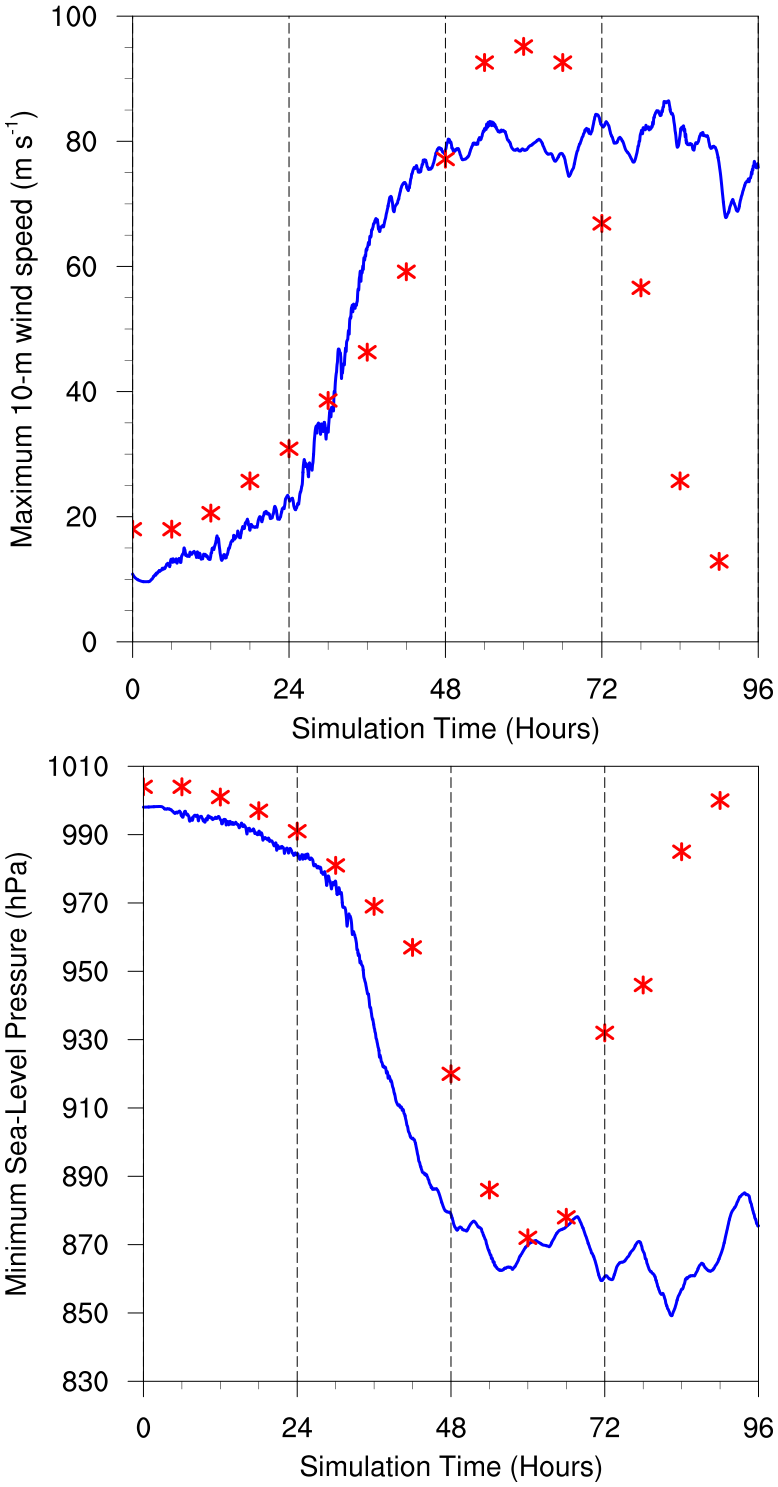
\includegraphics[width=19pc]{figures/vmax+pmin.png}}
\caption{The maximum 10-m wind speed (top panel; m s\textsuperscript{-1}) and minimum sea-level pressure (bottom panel; hPa) in the simulated storm (blue lines; plotted every minute) and from Hurricane Patricia's best track (red stars; plotted every six hours beginning at the time Patricia attained tropical storm intensity). The rapid weakening during the later stage of Patricia's lifetime was induced by landfall.}
\label{fig:vmax+pmin}
\end{figure}

%FIGURE 2%
\begin{figure}[ht]
\centerline{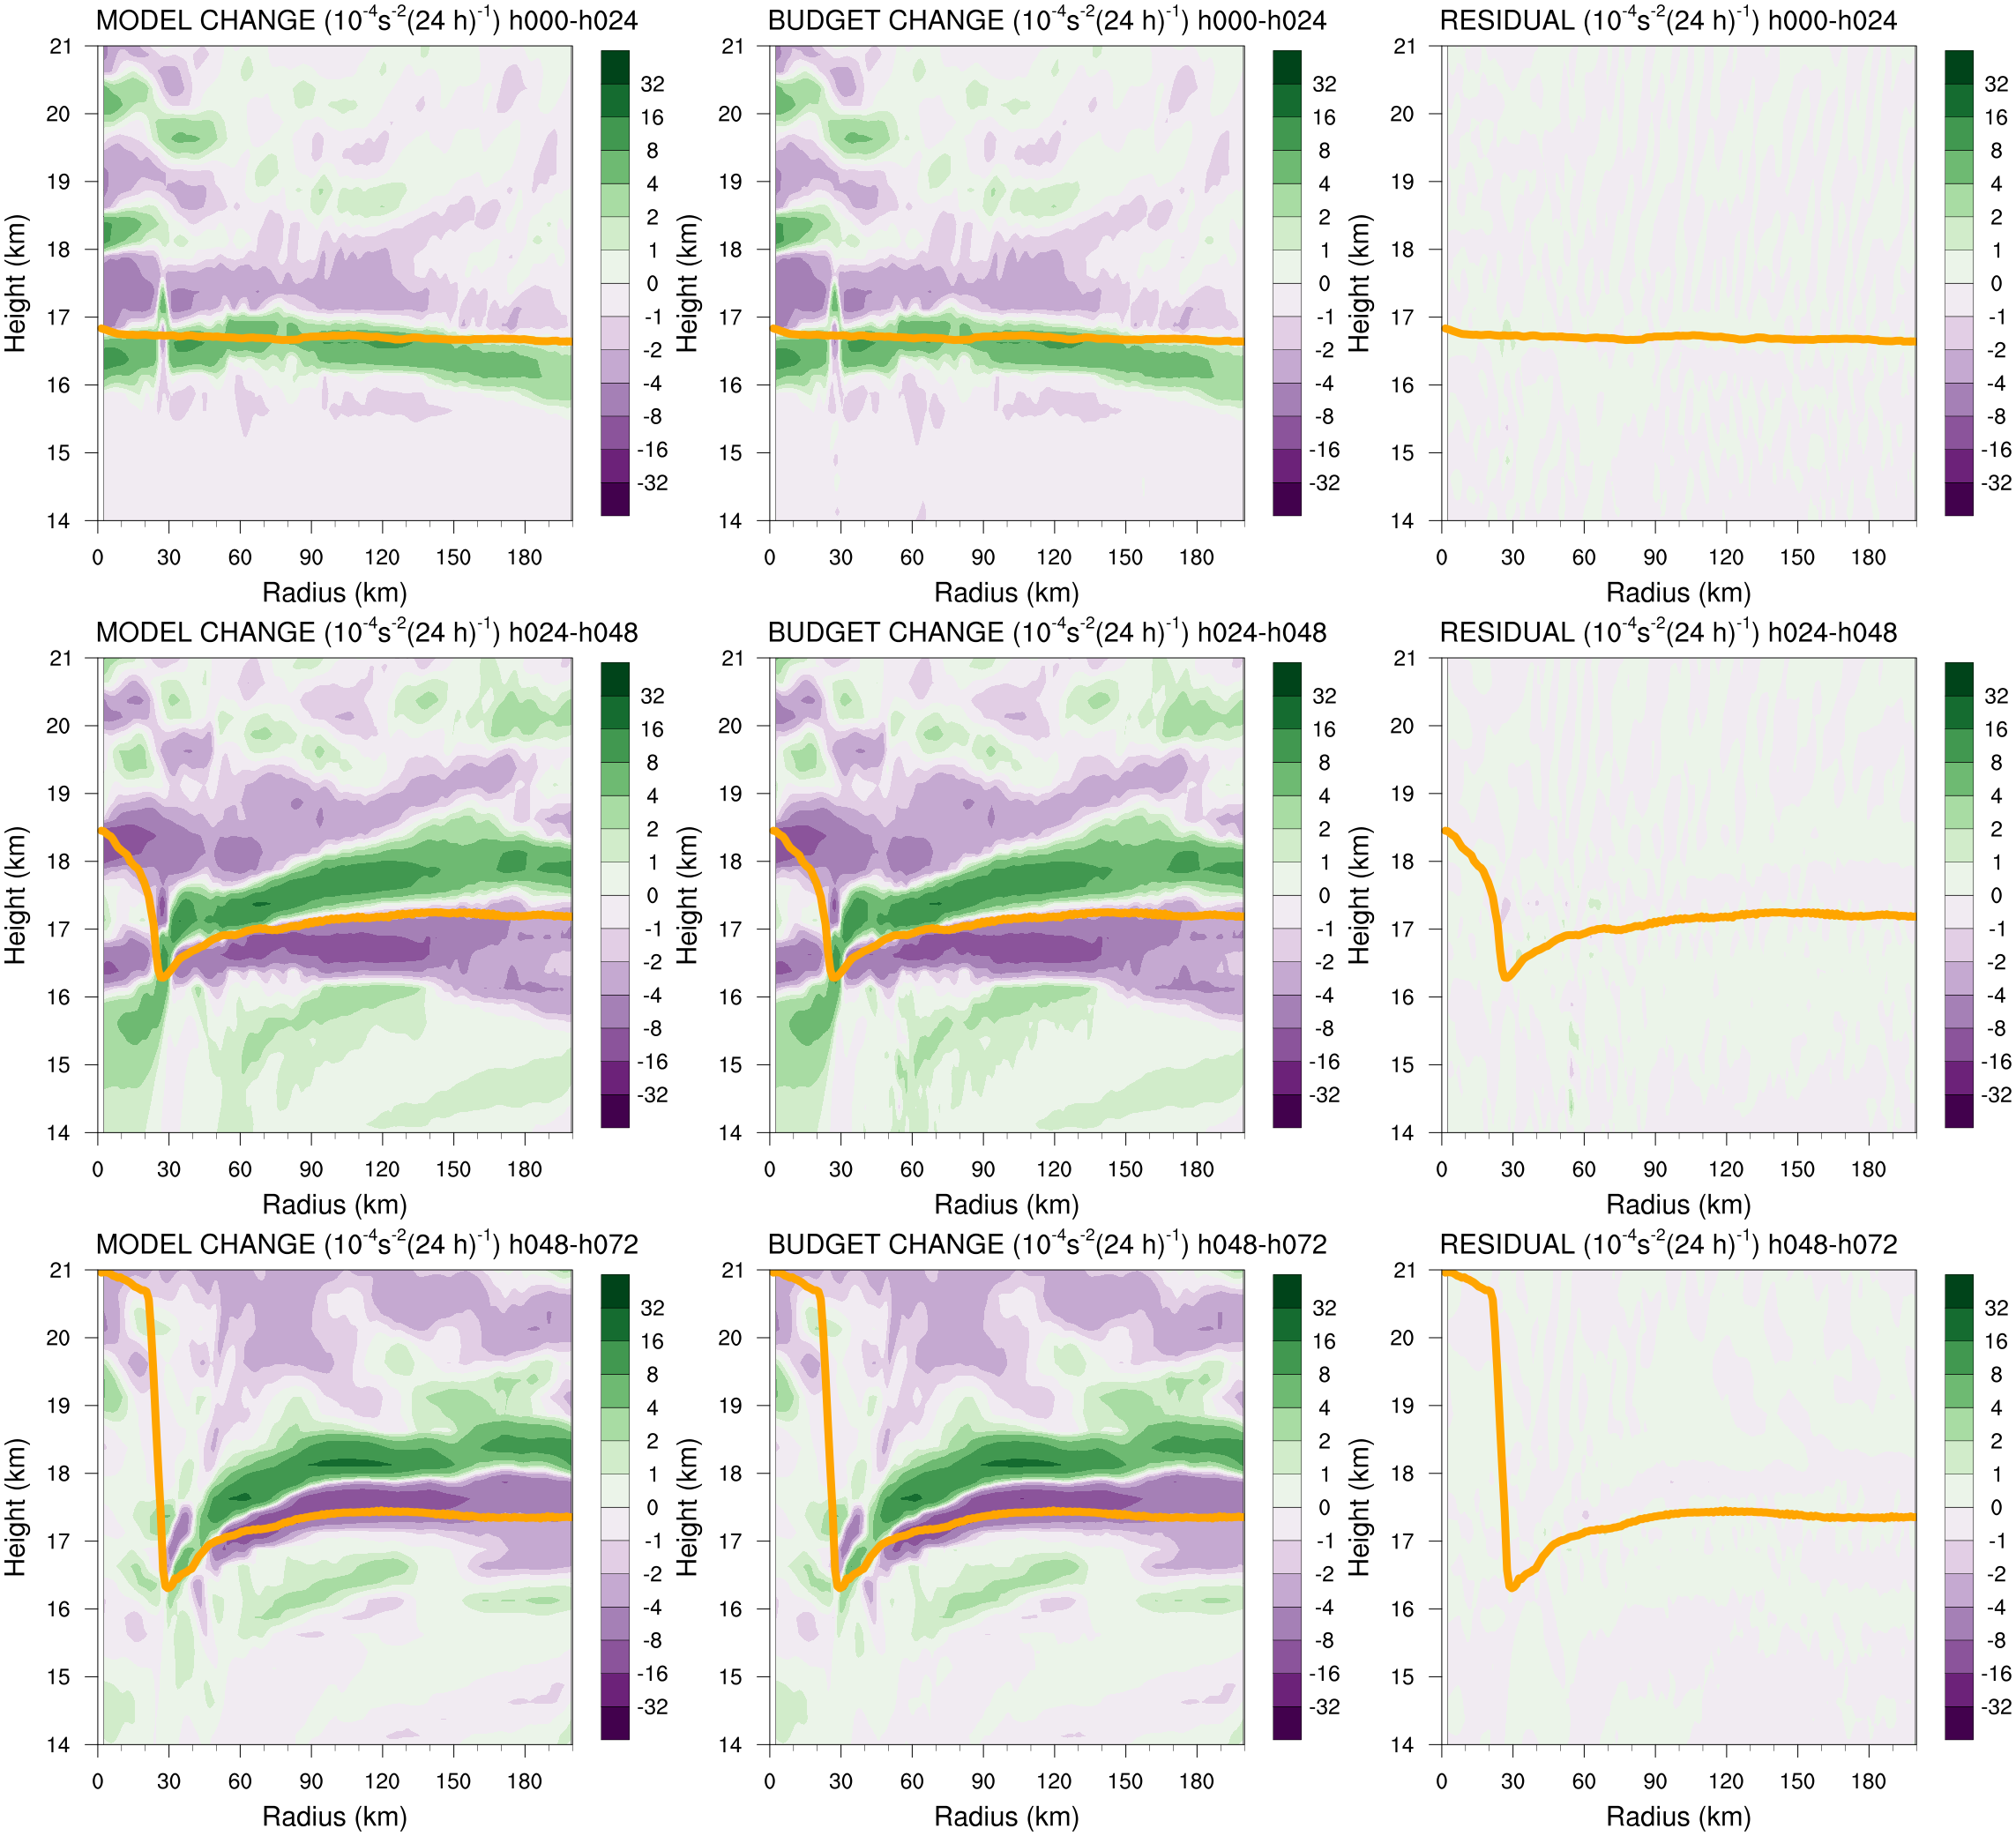
\includegraphics[width=39pc]{figures/mod+bud+res.png}}
\caption{Left panels: Twenty-four-hour changes in squared Brunt-V{\"a}is{\"a}l{\"a} frequency ($N^2$; 10\textsuperscript{-4} s\textsuperscript{-2}) computed using Eq.~\ref{eq:modelchange} over (top row) 0-24 hours, (middle row) 24-48 hours, (bottom row) 48-72 hours.
Middle Panels: The $N^2$ change over the same time periods computed using Eqs. \ref{eq:dn2dt}-\ref{eq:budgetchange}, %together with Eqs. \ref{eq:dn2dt}, \ref{eq:dthetadt}.
Right Panels: The budget residual over the same time periods, computed by subtracting the budget change (middle column) from the model change (left column).
Orange lines represent the cold-point tropopause height averaged over the same time periods.}
\label{fig:mod+bud+res}
\end{figure}

%FIGURE 3%
\begin{figure}[ht]
\centerline{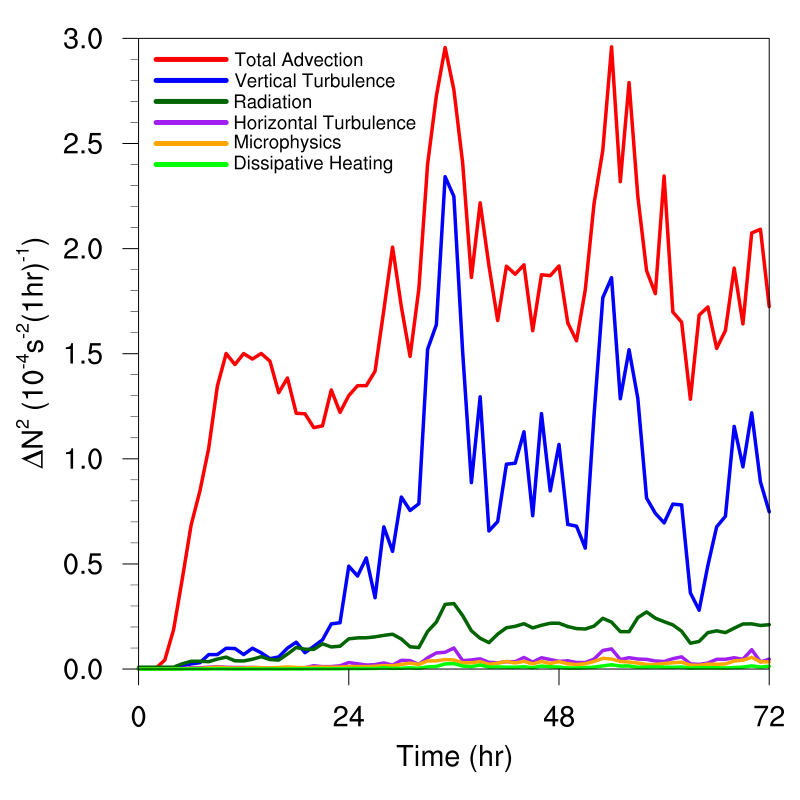
\includegraphics[width=19pc]{figures/AVG_budterms.png}}
\caption{Time series of the contribution of each of the budget terms to the time tendency of the squared Brunt-V{\"a}is{\"a}l{\"a} frequency ($N^2$; 10\textsuperscript{-4} s\textsuperscript{-2}).
For each budget term, the absolute value of the $N^2$ tendency is averaged temporally over 1-hour periods (using output every minute), and spatially in a region extending from 0 to 200 km radius and 14 to 21 km altitude.}
\label{fig:avgbudterms}
\end{figure}

%FIGURE 4%
\begin{figure*}[ht]
\centerline{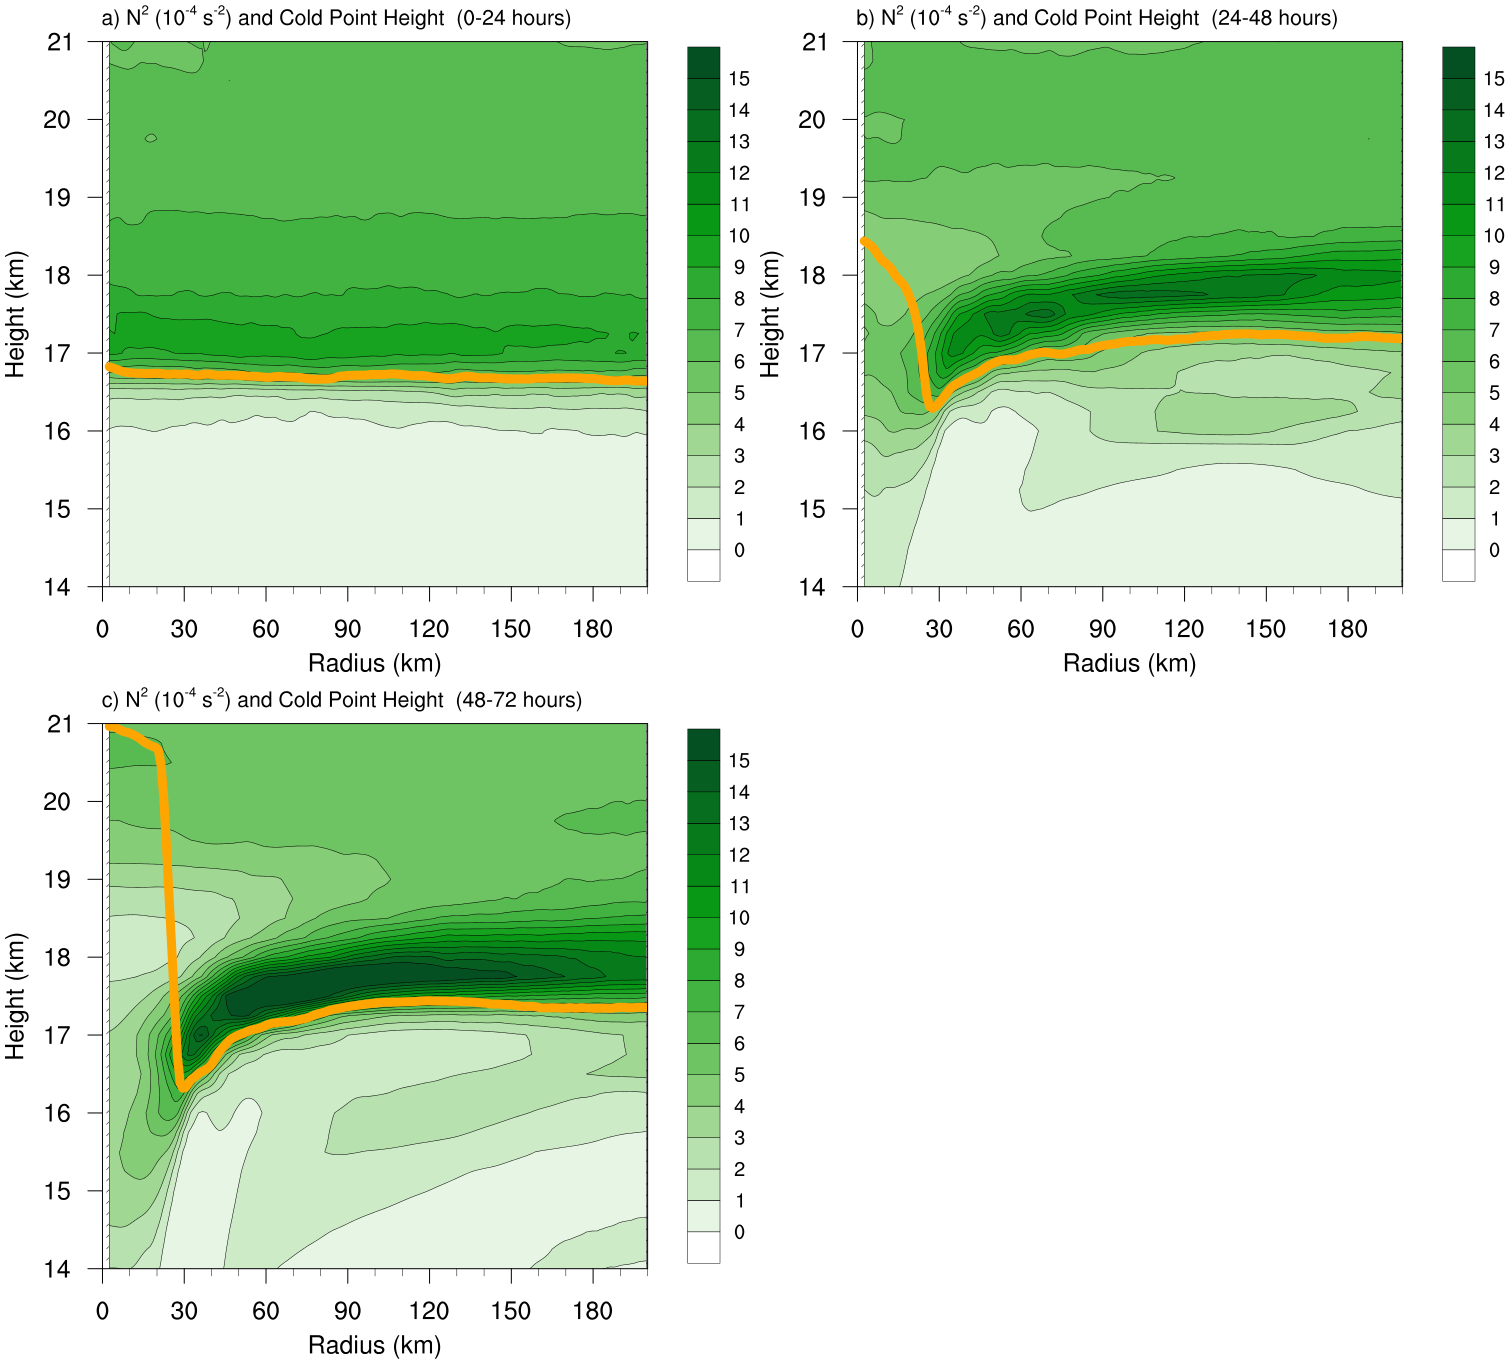
\includegraphics[width=39pc]{figures/n2-24hr-avgs.png}}
\caption{Twenty-four-hour averages of squared Brunt-V{\"a}is{\"a}l{\"a} frequency ($N^2$; 10\textsuperscript{-4} s\textsuperscript{-2}) over (a) 0-24 hours, (b) 24-48 hours, (c) 48-72 hours.
Orange lines represent the cold-point tropopause height averaged over the same time periods.}
\label{fig:n2-24hr-avgs}
\end{figure*}

%FIGURE 5%
\begin{figure*}[ht]
\centerline{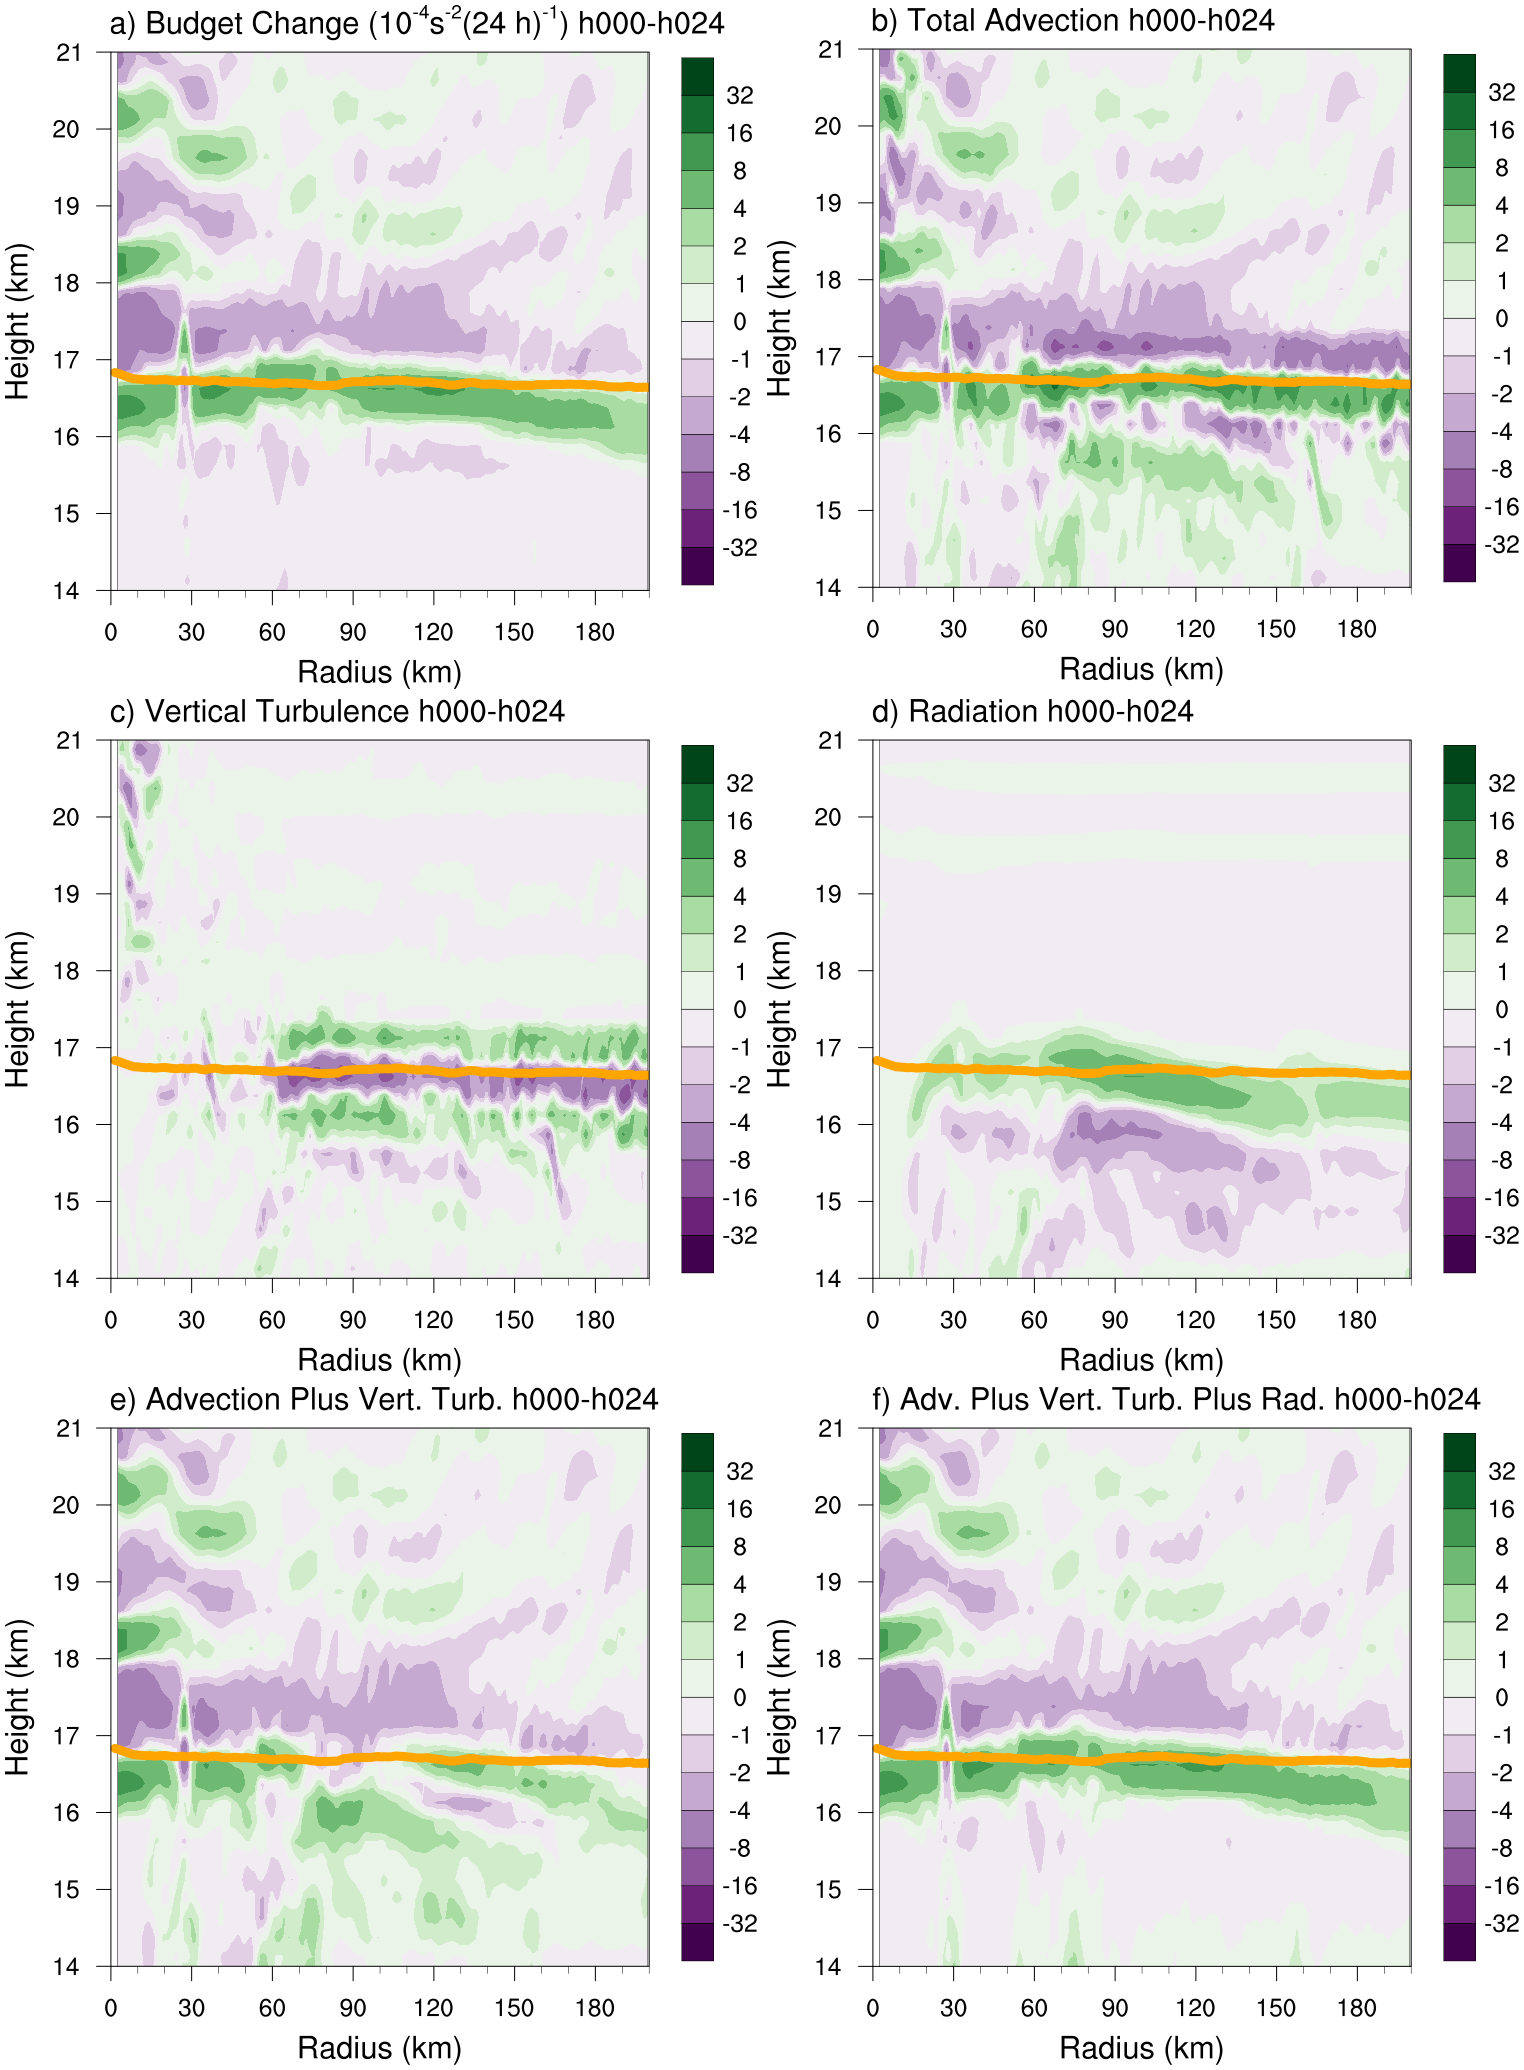
\includegraphics[width=39pc]{figures/h000-h024-budgetterms.png}}
\end{figure*}
\begin{figure}
\caption{(a) Total change in $N^2$ over the 0-24-hour period (10\textsuperscript{-4} s\textsuperscript{-2} (24 h)\textsuperscript{-1}) and the contributions to that change from (b) the sum of horizontal and vertical advection, (c) vertical turbulence, (d) longwave and shortwave radiation, (e) the sum of horizontal advection, vertical advection, and vertical turbulence, and (f) the sum of horizontal advection, vertical advection, vertical turbulence, and longwave and shortwave radiation.
Green shading indicates regions of stabilization and purple shading indicates regions of destabilization.
Orange lines represent the cold-point tropopause height averaged over the 0-24-hour period.}
\label{fig:stab-00-24}
\end{figure}

%FIGURE 6%
\begin{figure*}[ht]
\centerline{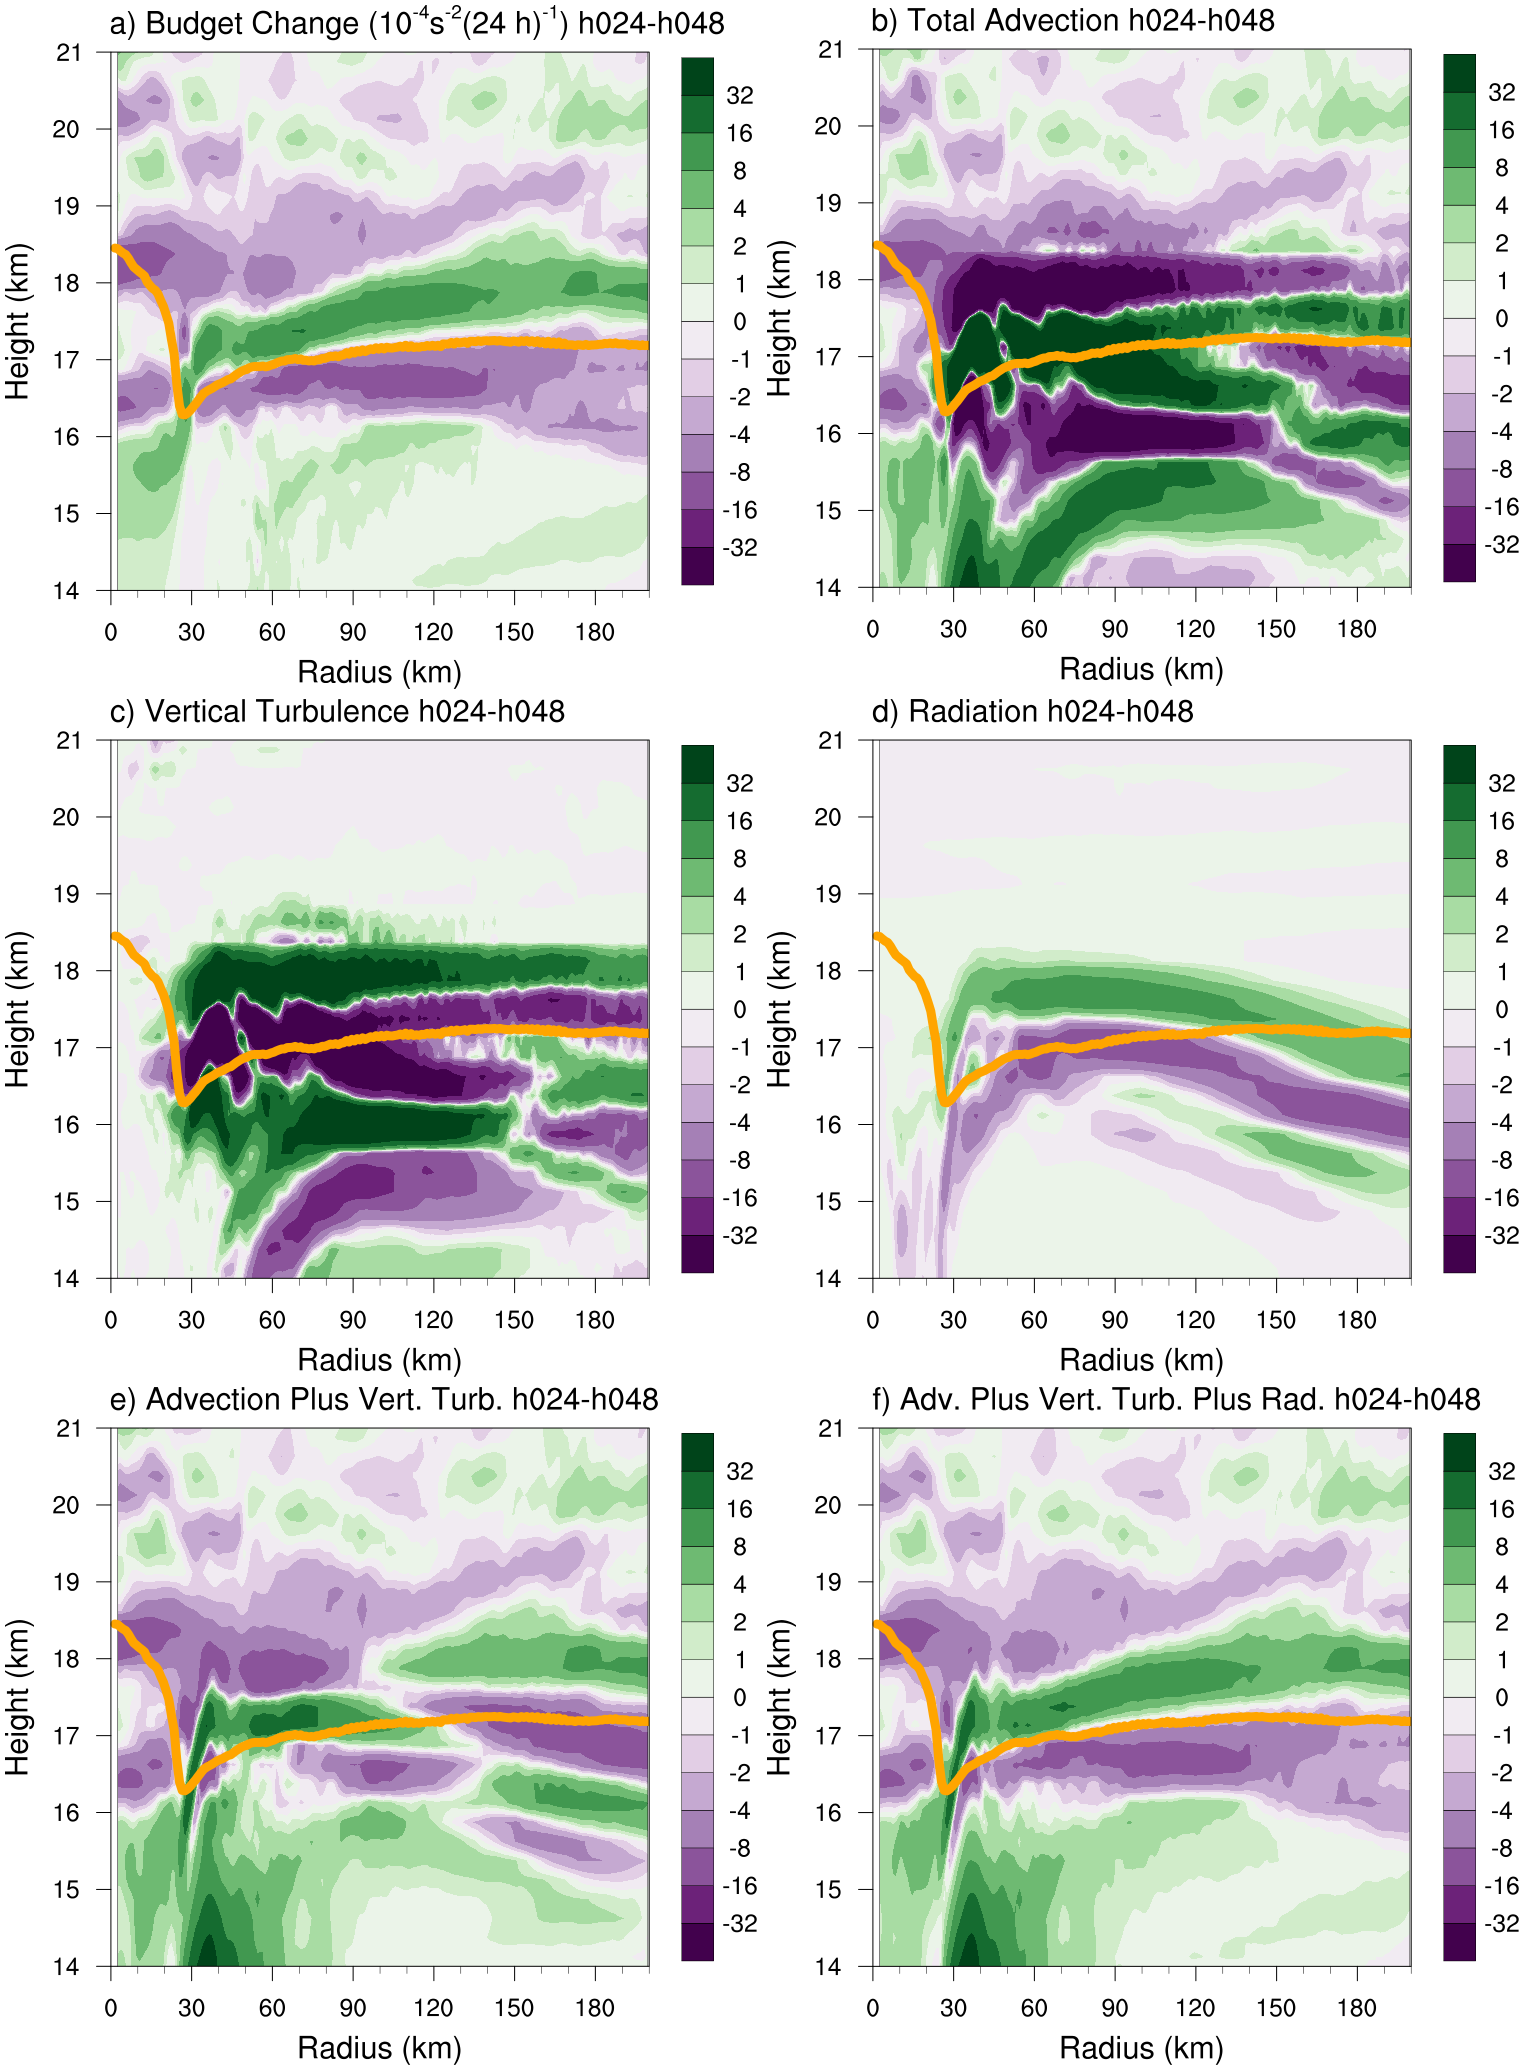
\includegraphics[width=39pc]{figures/h024-h048-budgetterms.png}}
\caption{As in Fig.~\ref{fig:stab-00-24}, but for the 24-48-hour period.}
\label{fig:stab-24-48}
\end{figure*}

%FIGURE 7%
\begin{figure*}[ht]
\centerline{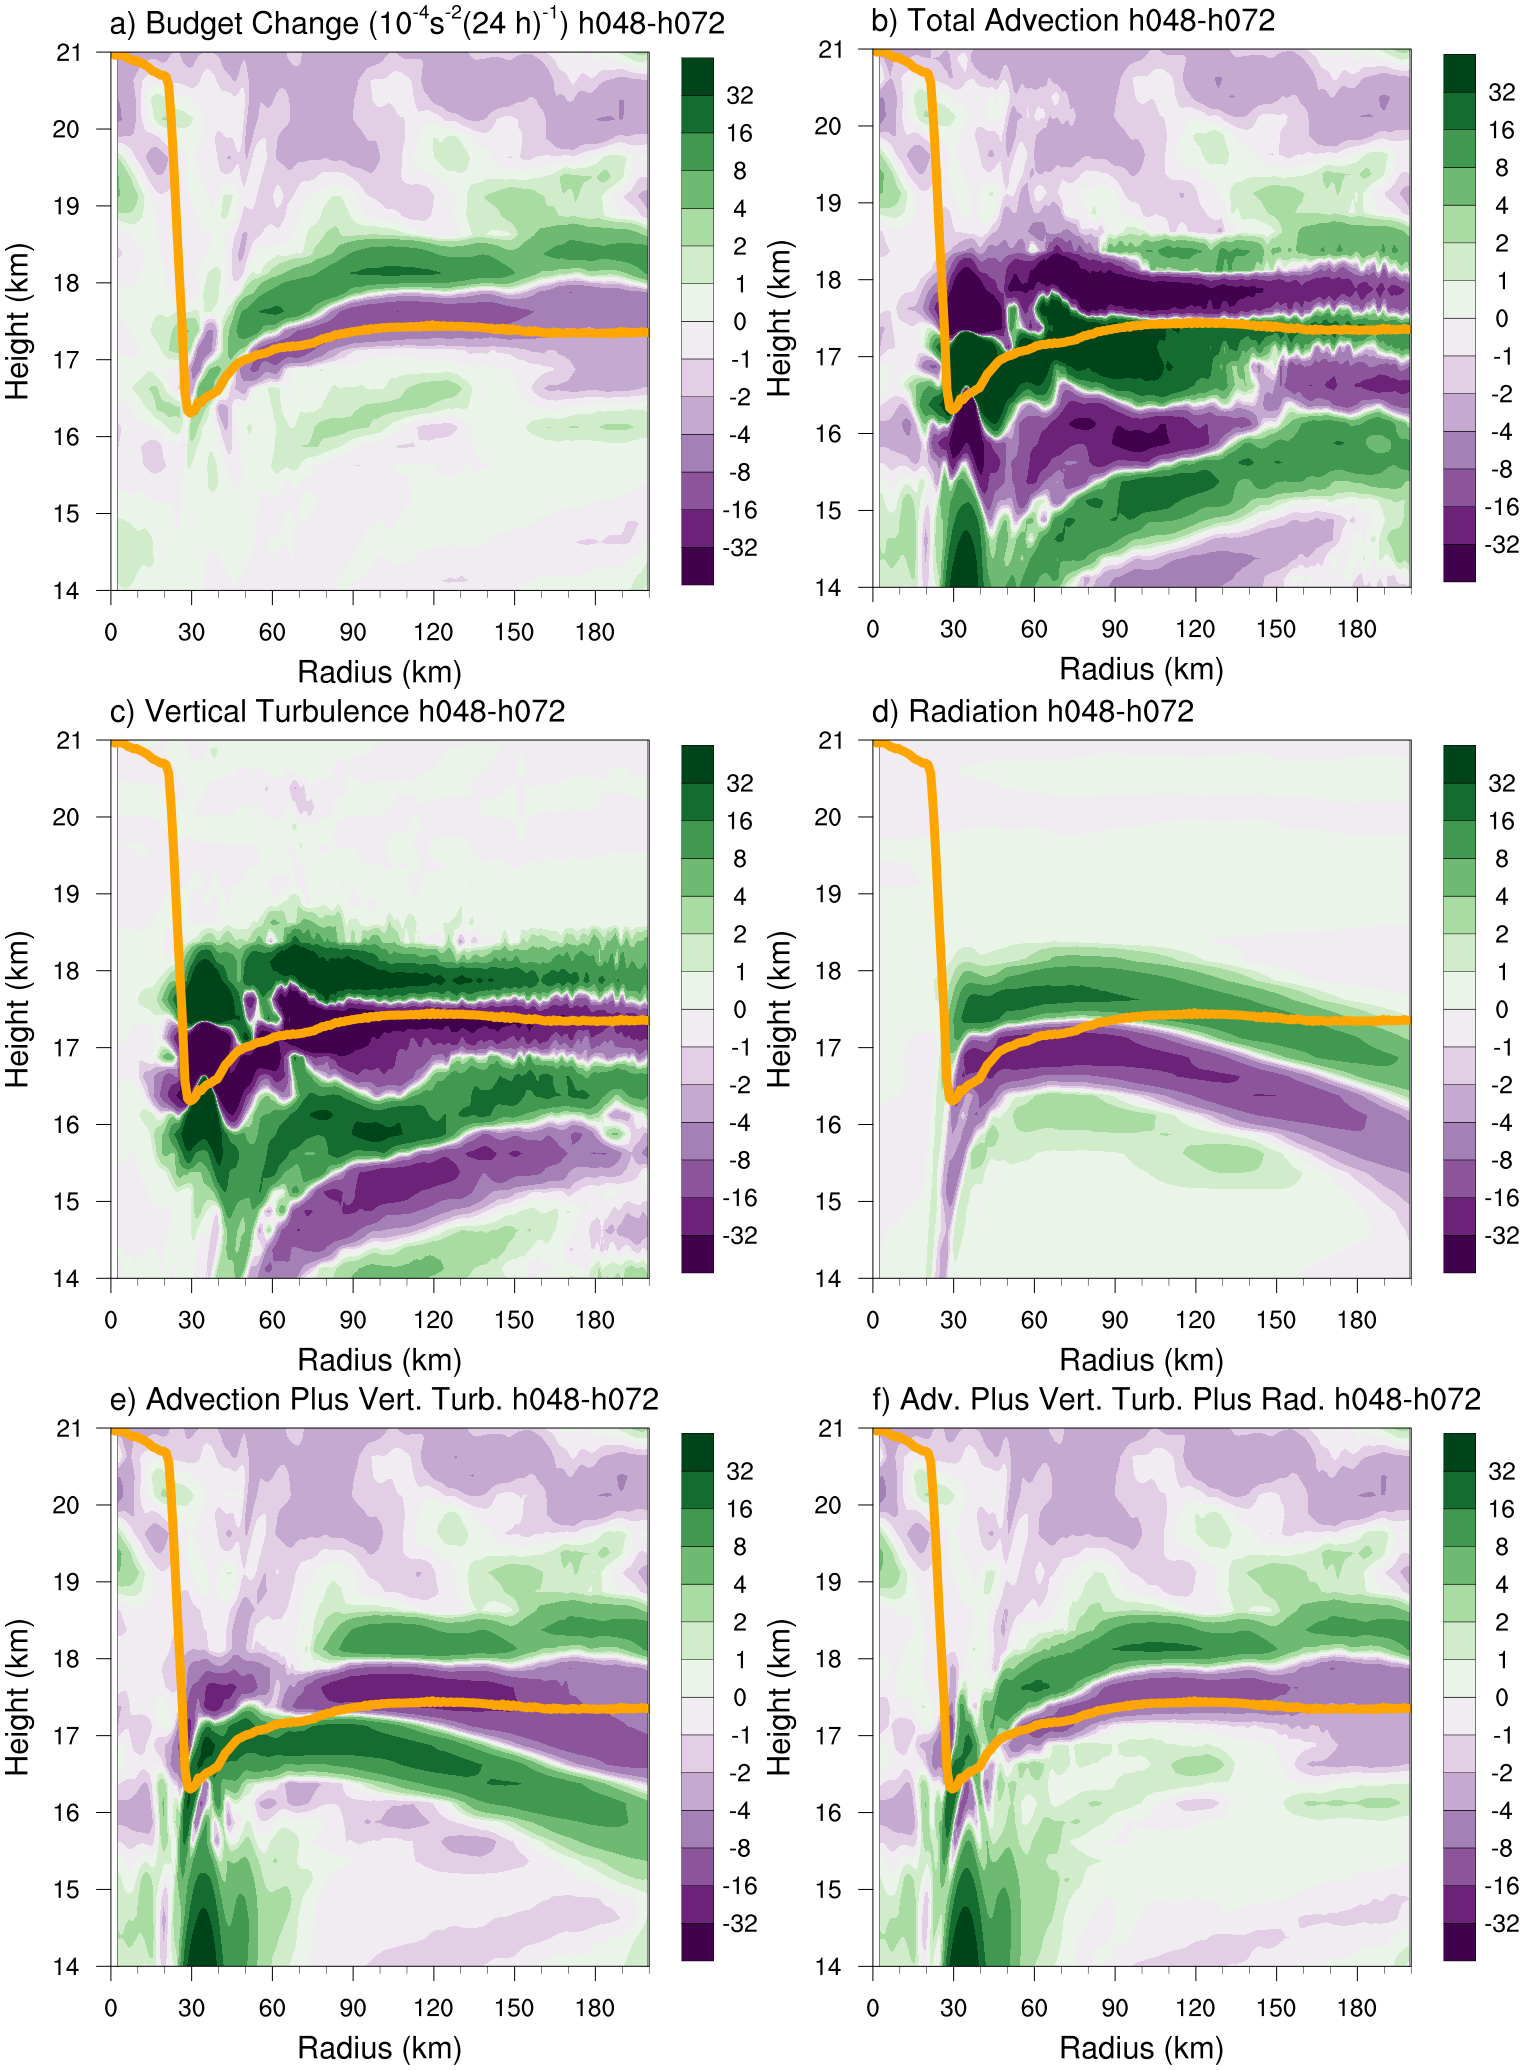
\includegraphics[width=39pc]{figures/h048-h072-budgetterms.png}}
\caption{As in Fig.~\ref{fig:stab-00-24}, but for the 48-72-hour period.}
\label{fig:stab-48-72}
\end{figure*}

%FIGURE 8%
\begin{figure*}[ht]
\centerline{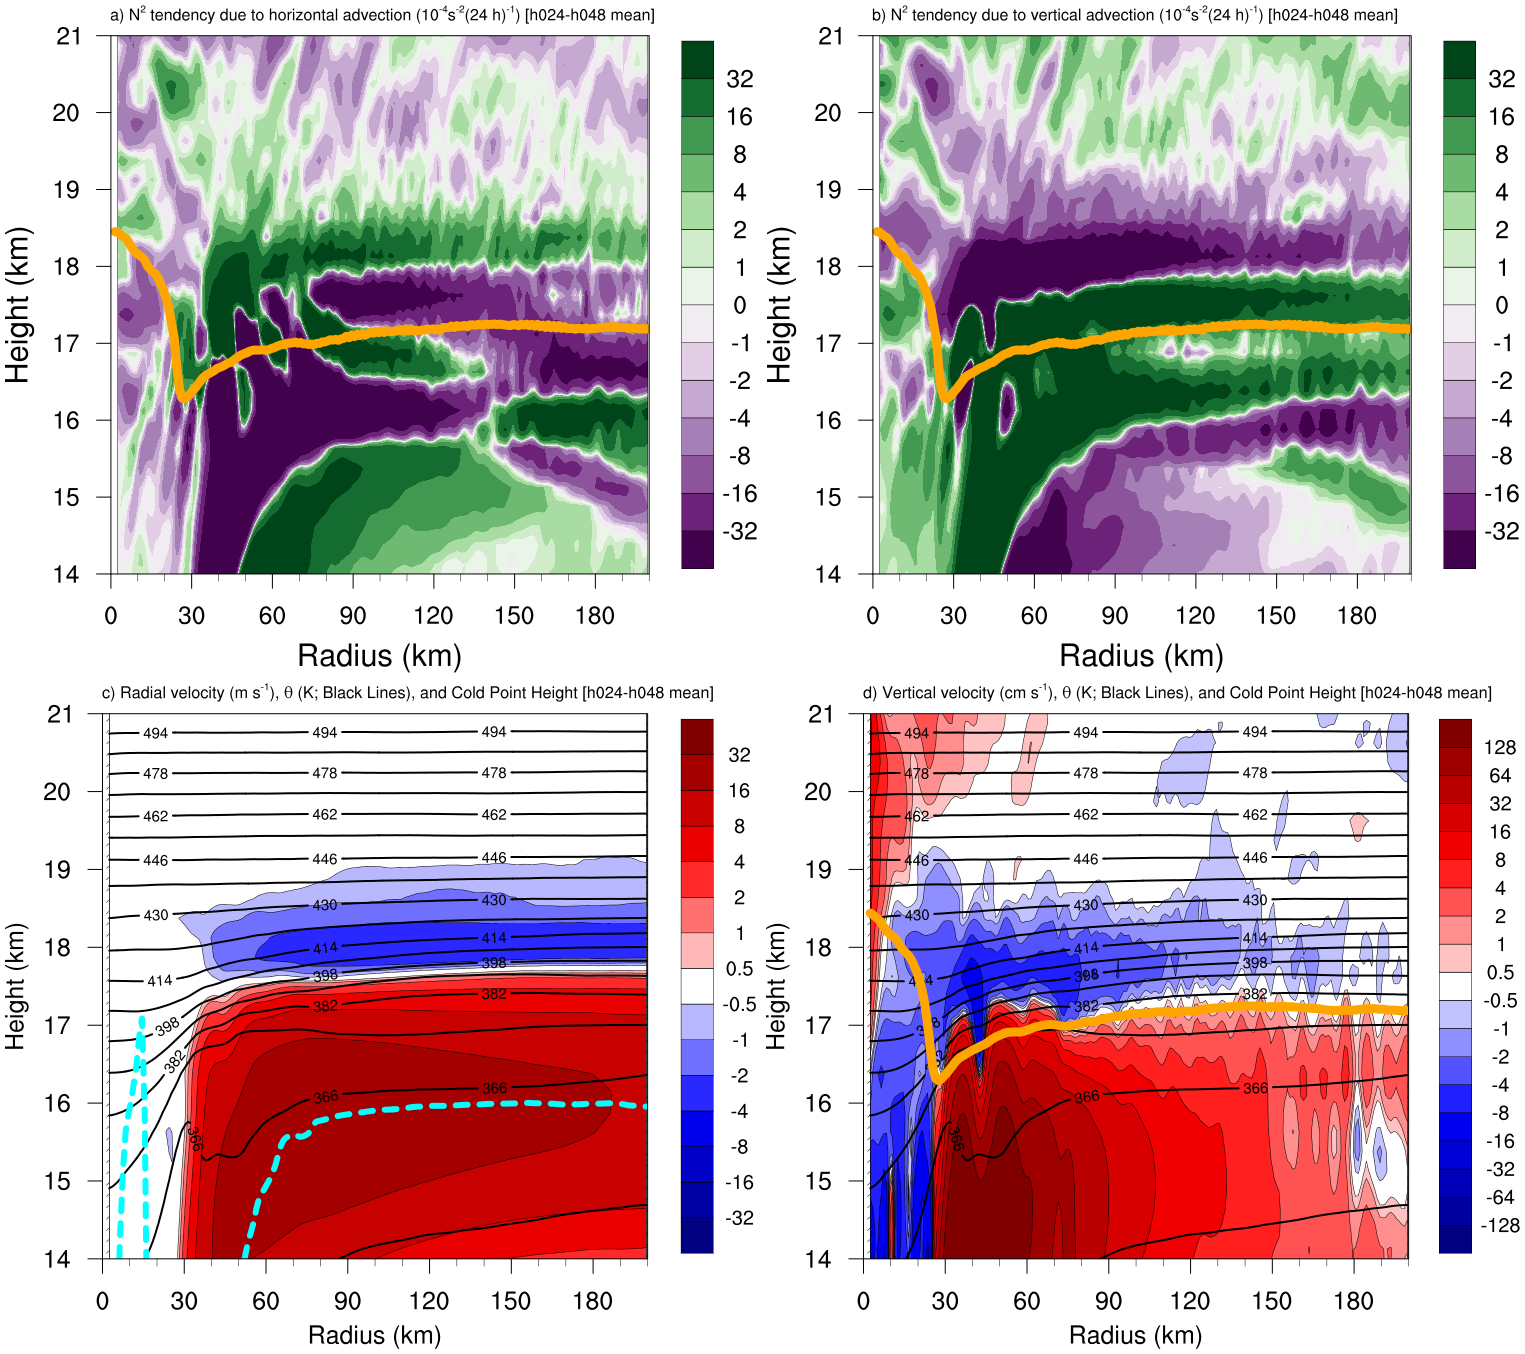
\includegraphics[width=39pc]{figures/h024-h048-adv.png}}
\caption{The contributions to the change in $N^2$ over the 24-48-hour period (10\textsuperscript{-4} s\textsuperscript{-2} (24 h)\textsuperscript{-1}) by (a) horizontal advection and (b) vertical advection. (c) The radial velocity (m s\textsuperscript{-1}; filled contours), potential temperature (K; thick black contours), cold-point tropopause height (orange line), and level of maximum outflow (dashed cyan line) averaged over the 24-48-hour period. (d) The vertical velocity (cm s\textsuperscript{-1}; filled contours), potential temperature (K; thick black contours), and cold-point tropopause height (orange line) averaged over the 24-48-hour period.}
%\caption{As in Fig. \ref{fig:adv-00-24}, but for the 24-48-hour period.}
\label{fig:adv-24-48}
\end{figure*}

%FIGURE 9%
%\begin{figure*}[ht]
%\centerline{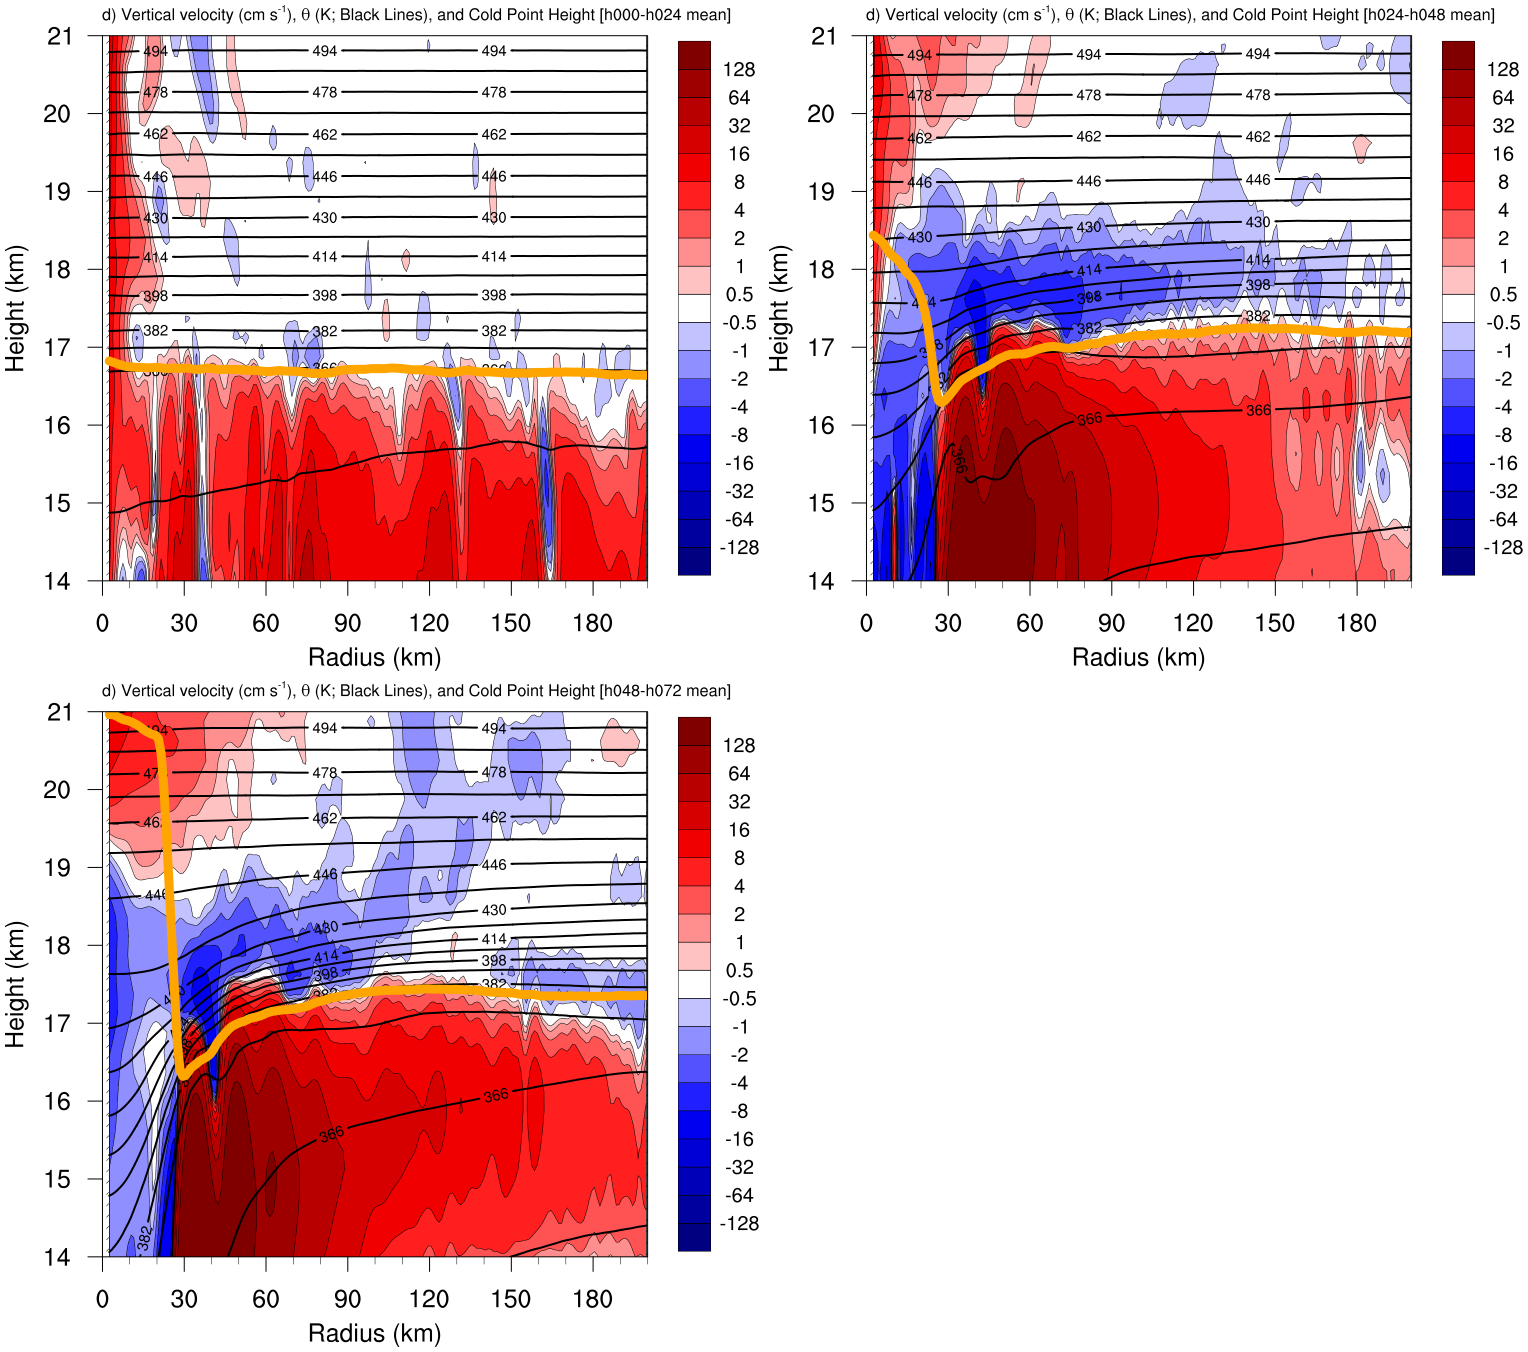
\includegraphics[width=39pc]{figures/w.png}}
%\caption{Vertical velocity (cm s\textsuperscript{-1}; filled contours), potential temperature (K; thick black contours), and cold-point tropopause height (orange lines) averaged over (a) 0-24 hours, (b) 24-48 hours, and (c) 48-72 hours.}
%\label{fig:w}
%\end{figure*}

%FIGURE 10%
%\begin{figure*}[ht]
%\centerline{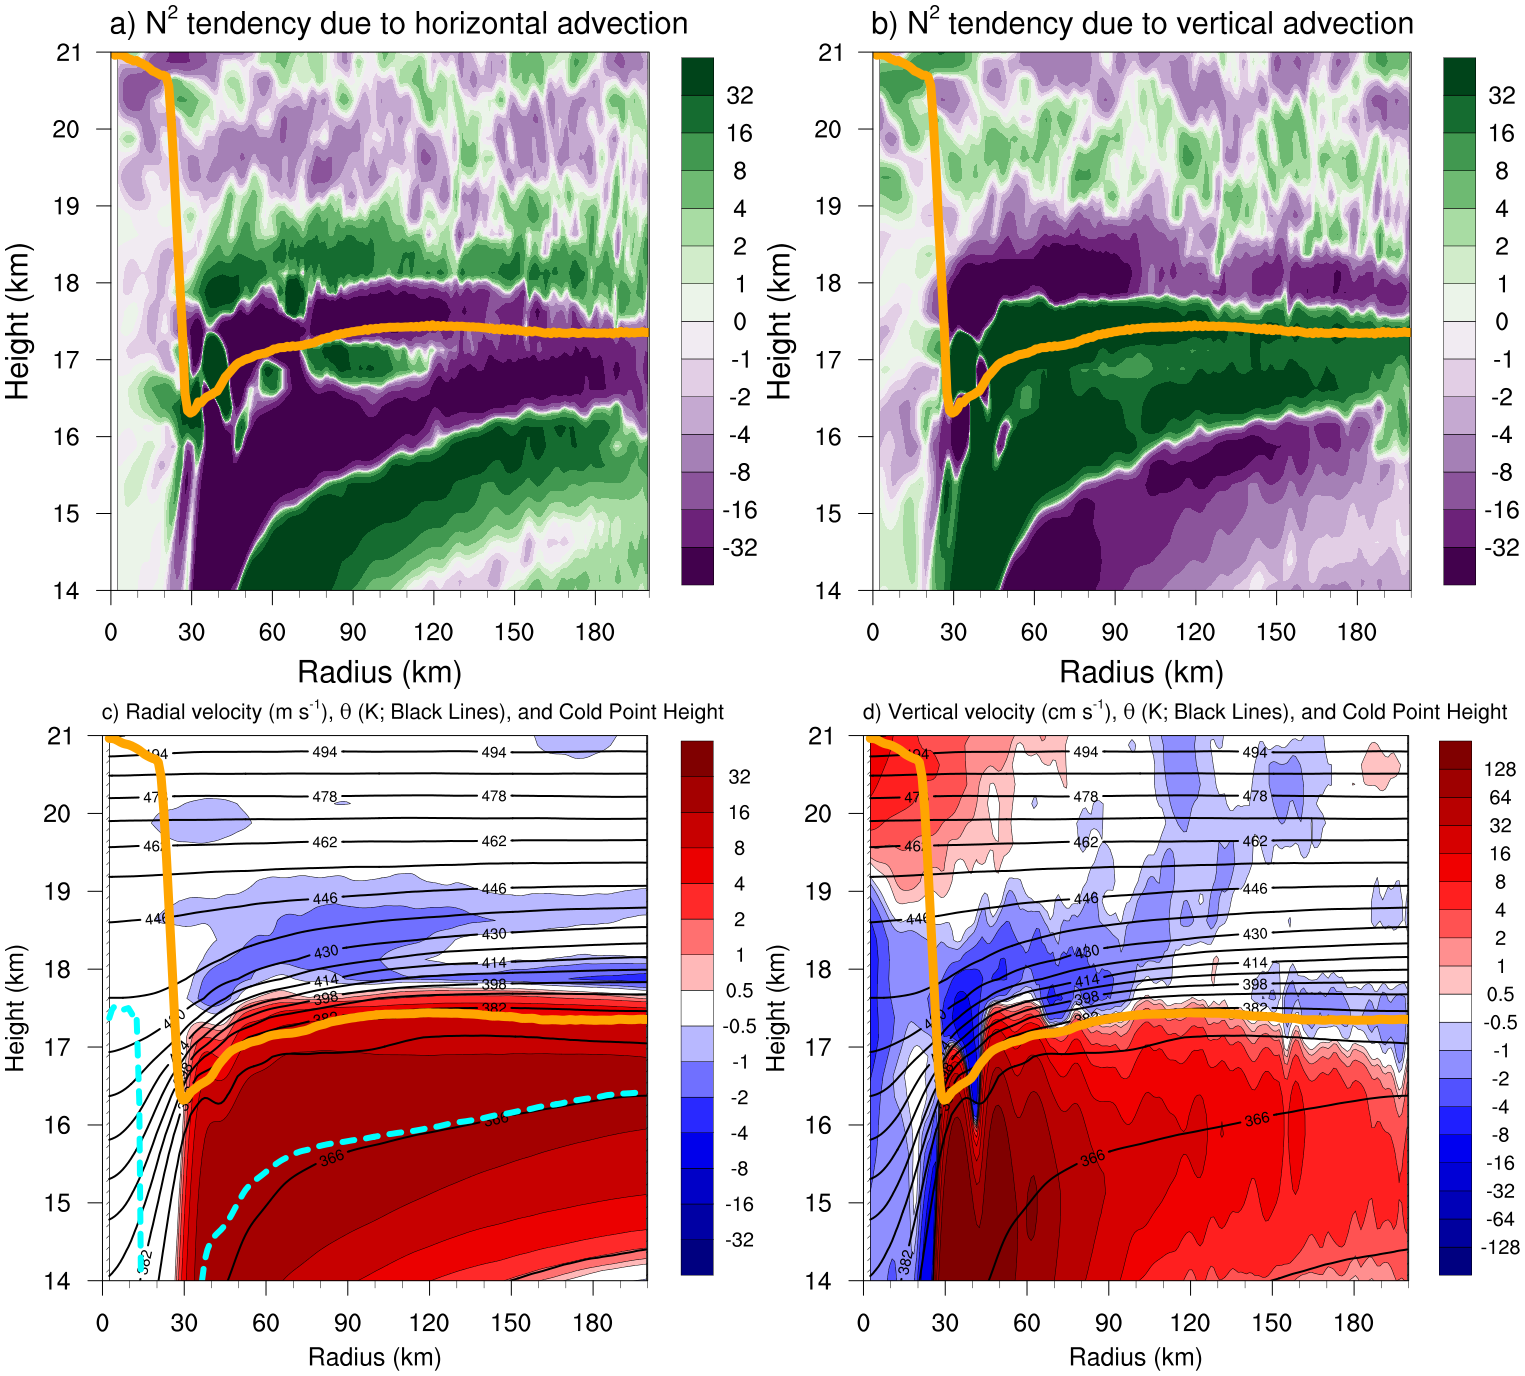
\includegraphics[width=39pc]{figures/h048-h072-adv.png}}
%\caption{As in Fig. \ref{fig:adv-00-24}, but for the 48-72-hour period.}
%\label{fig:adv-48-72}
%\end{figure*}

%FIGURE 9%
\begin{figure*}[ht]
\centerline{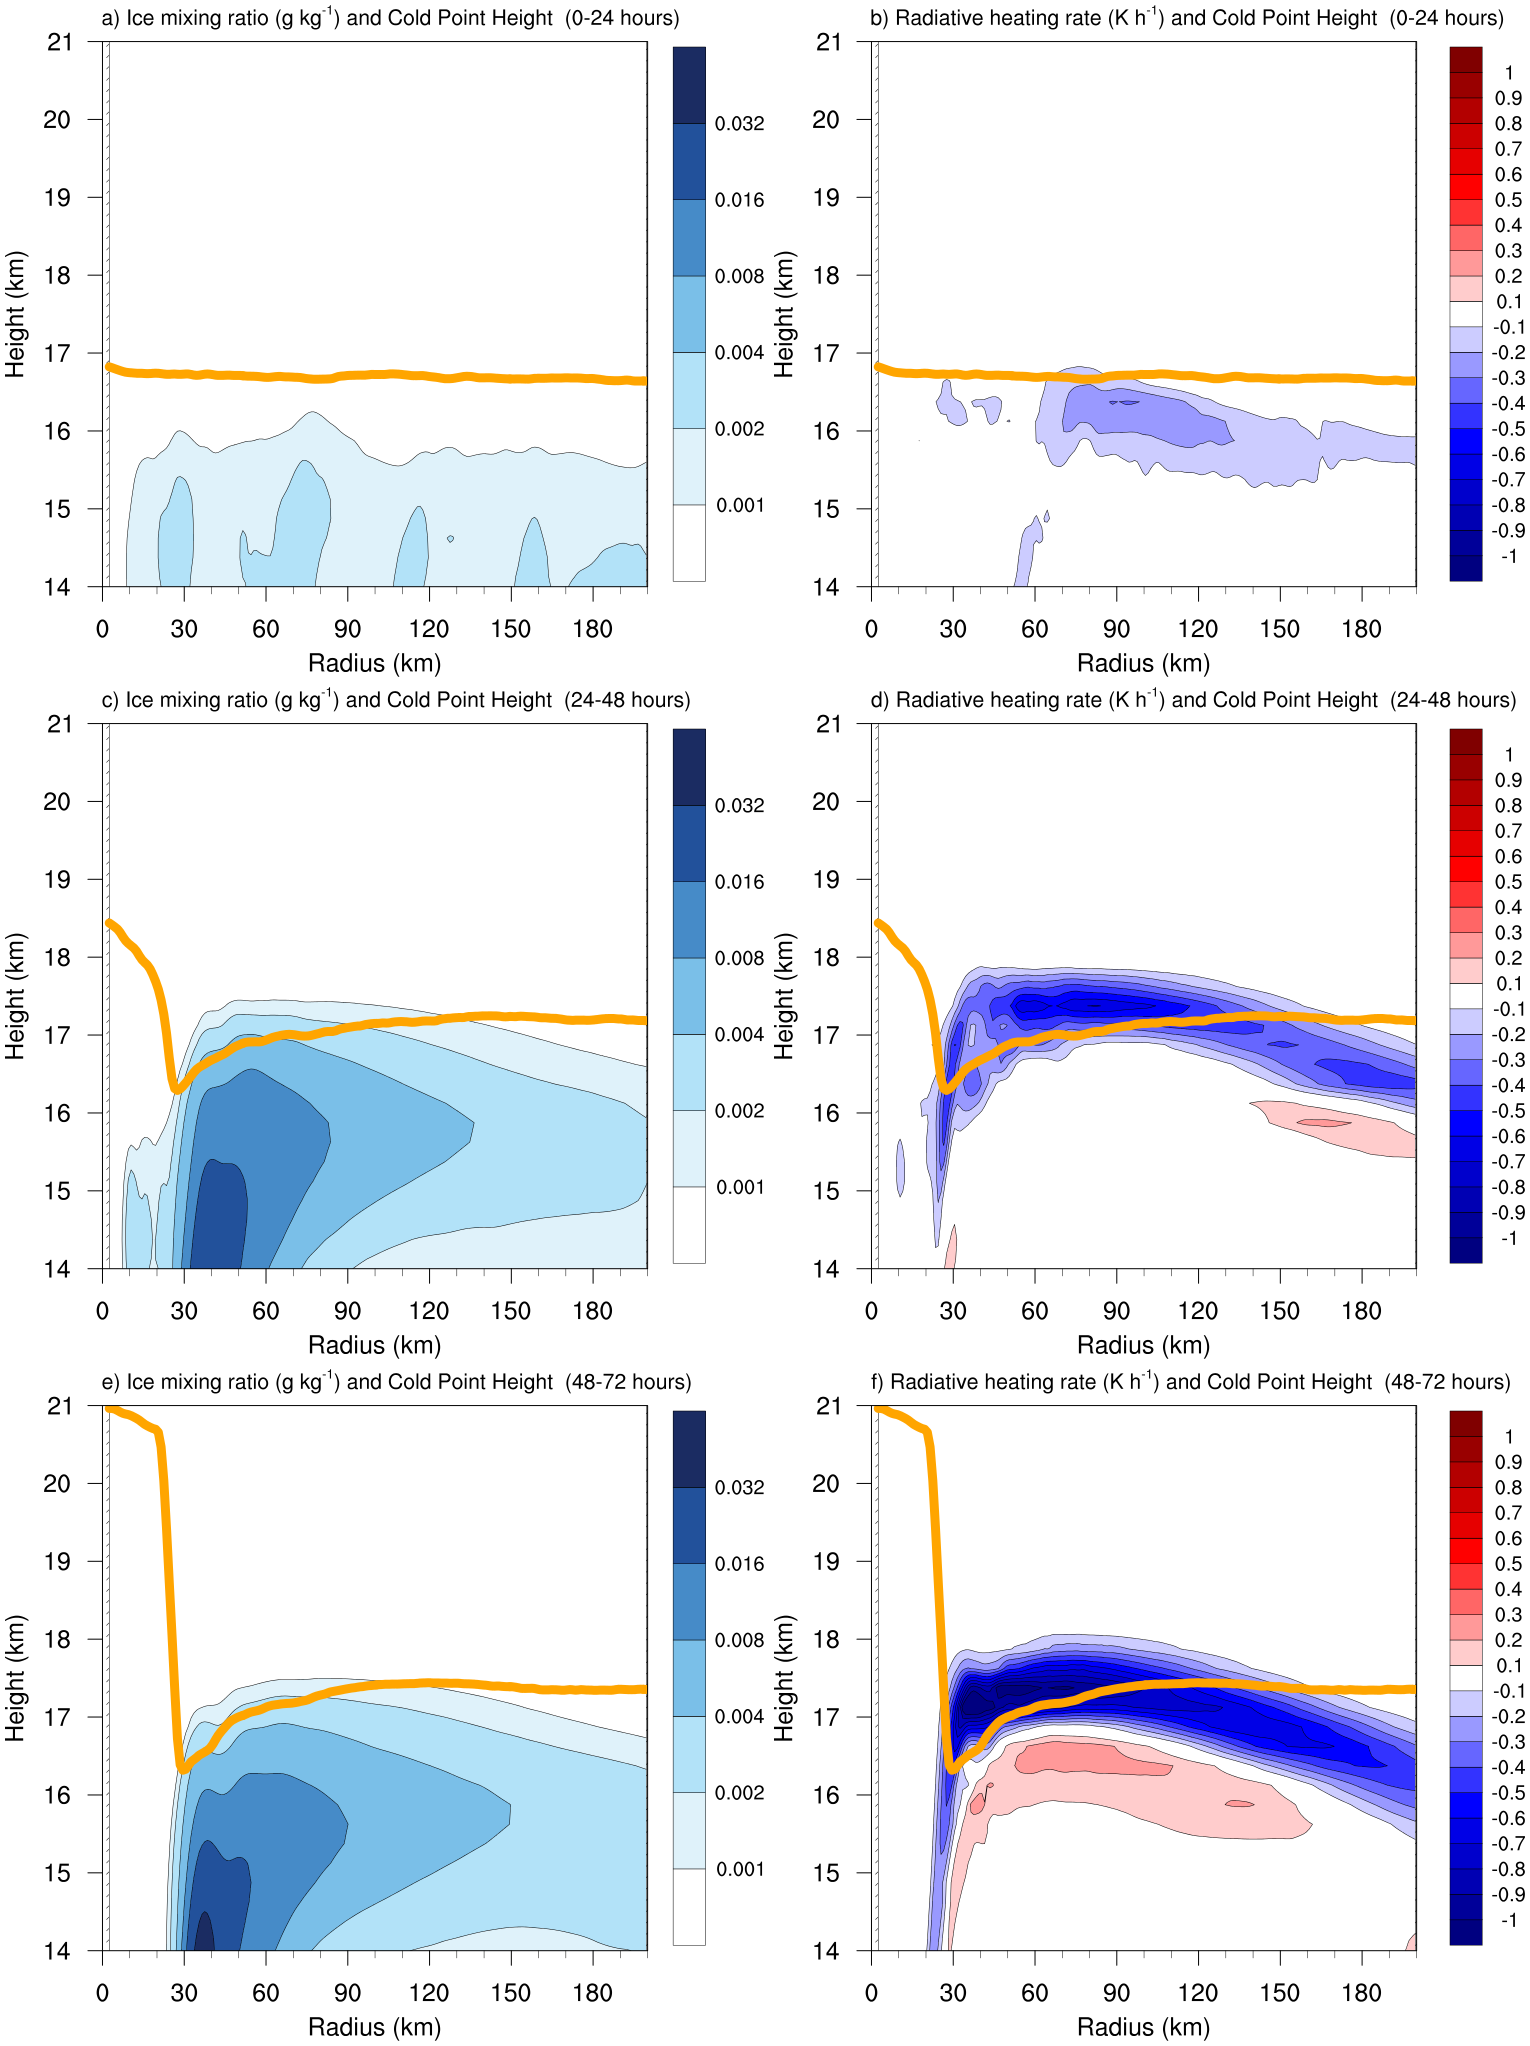
\includegraphics[width=39pc]{figures/qi+radten.png}}
\end{figure*}
\begin{figure}
\caption{Ice mixing ratio (g kg\textsuperscript{-1}) and cold-point tropopause height (orange lines) averaged over (a) 0-24 hours, (c) 24-48 hours, and (e) 48-72 hours. Radiative heating rate (K h\textsuperscript{-1}) and cold-point tropopause height (orange lines) averaged over (b) 0-24 hours, (d) 24-48 hours, and (f) 48-72 hours.}
\label{fig:qi+radten}
\end{figure}

%FIGURE 10%
\begin{figure*}[ht]
\centerline{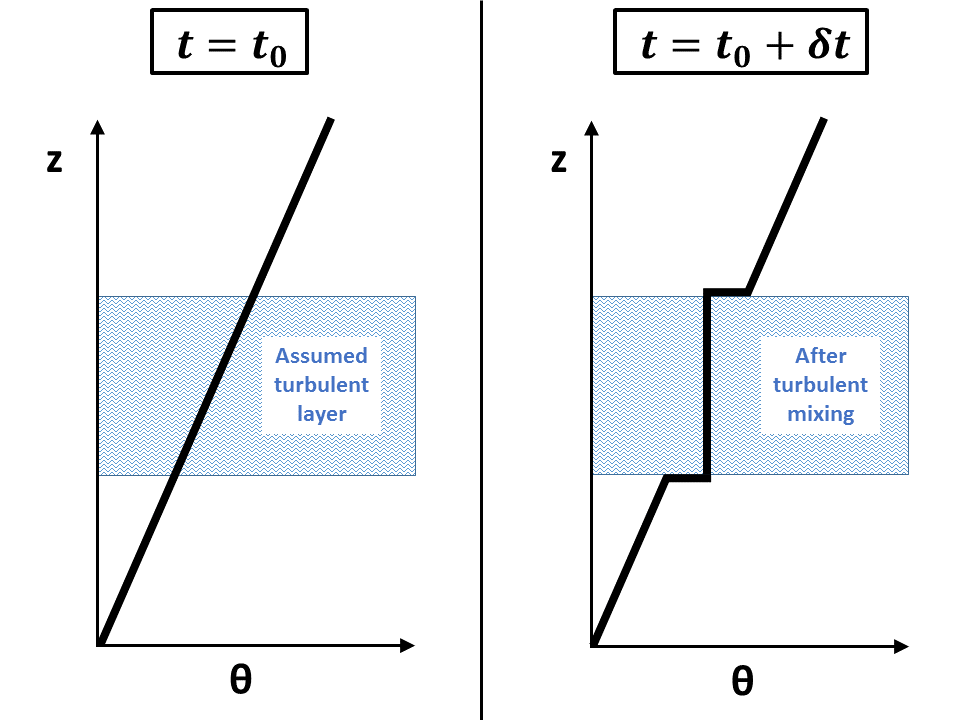
\includegraphics[width=39pc]{figures/Schematic2.png}}
   \caption{Schematic diagram of the effect of turbulent mixing on the vertical profile of potential temperature ($\theta$). At the initial time (left panel), potential temperature is assumed to increase with height at a constant rate (thick black line). The imposition of turbulence within a portion of the layer (blue hatching) adjusts the potential temperature profile toward the mean initial value of that layer. After a period of mixing (right panel) the potential temperature in the mixed layer does not vary with height, but just above and just below the mixed layer, it rapidly increases with height.}
\label{fig:schematic}
\end{figure*}

%FIGURE 11%
\begin{figure*}[ht]
\centerline{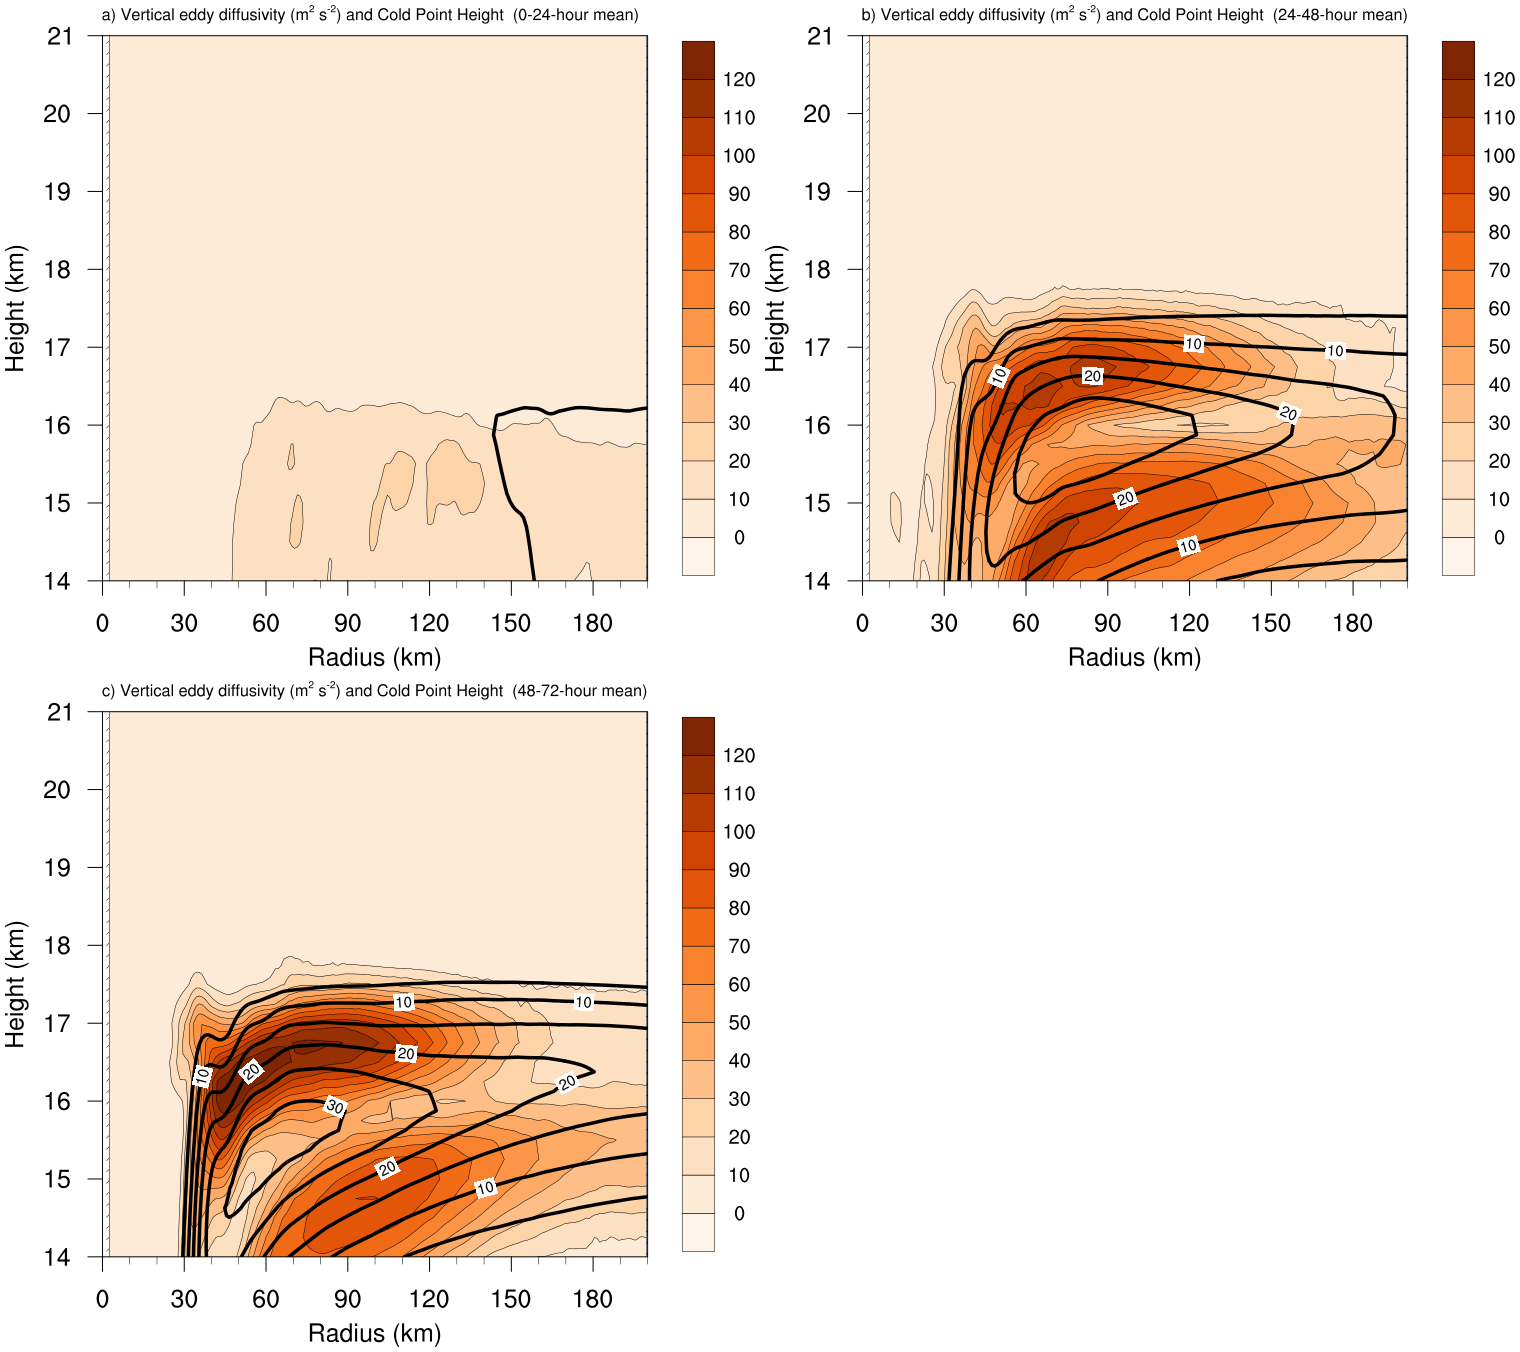
\includegraphics[width=39pc]{figures/khvten.png}}
\caption{Vertical eddy diffusivity (m\textsuperscript{2} s\textsuperscript{-2}; filled contours), cold-point tropopause height (cyan lines), and radial velocity (m s\textsuperscript{-1}; thick black lines) averaged over (a) 0-24 hours, (b) 24-48 hours, and (c) 48-72 hours.}
\label{fig:diff}
\end{figure*}

%FIGURE 12%
\begin{figure*}[ht]
\centerline{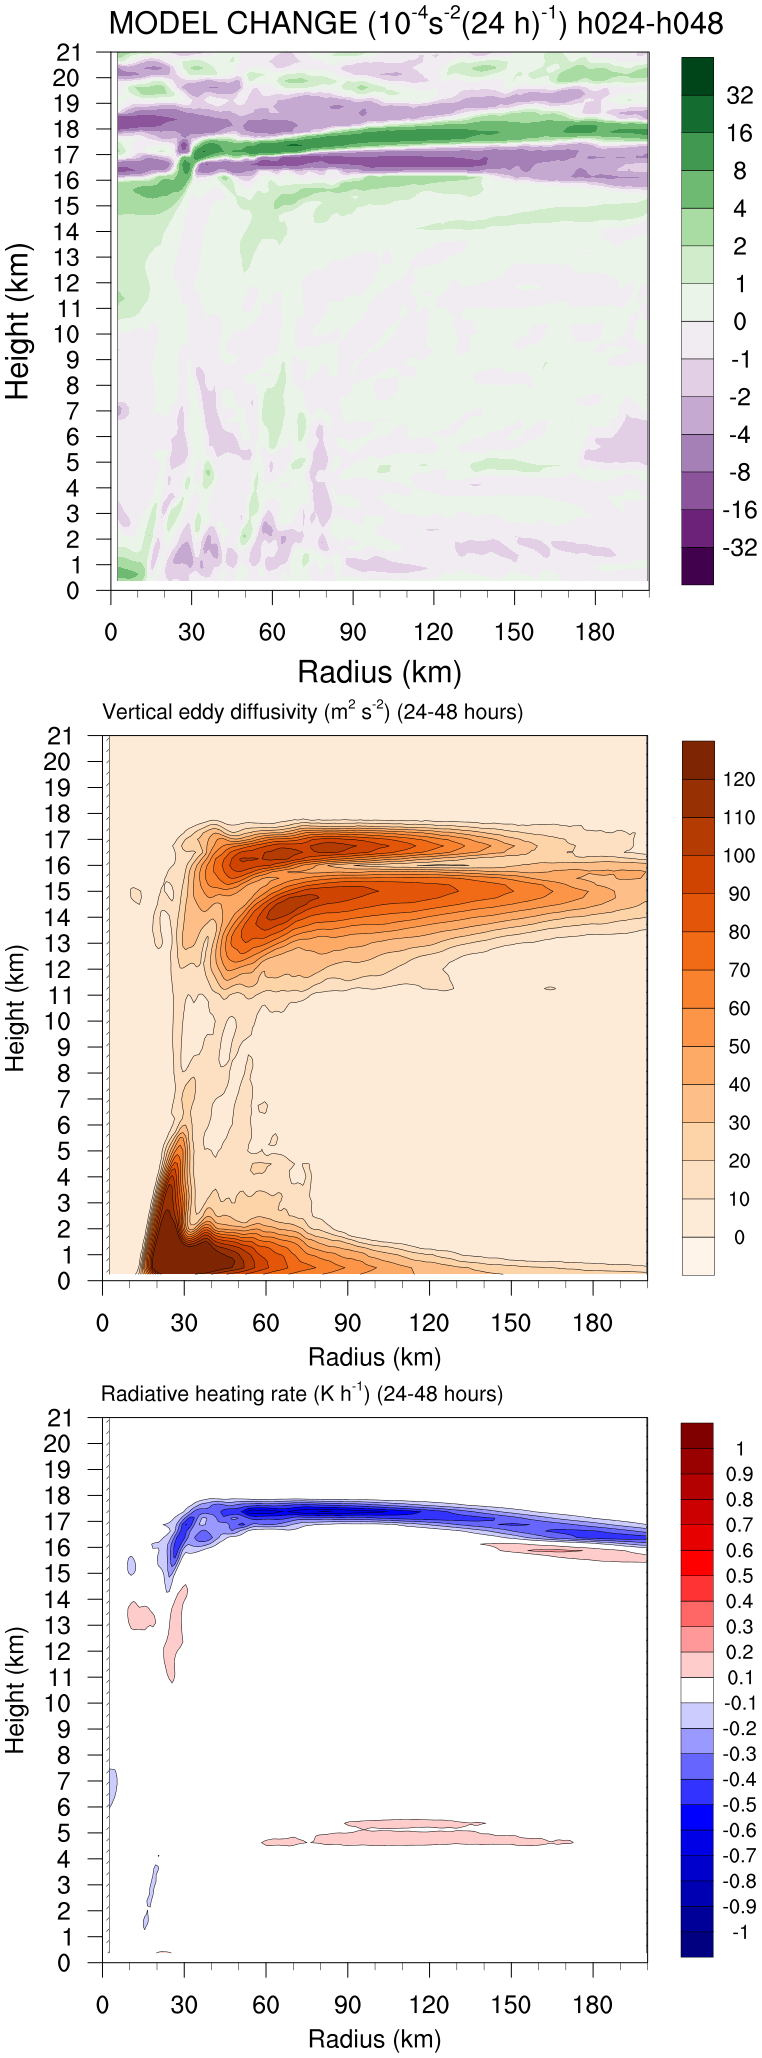
\includegraphics[width=19pc]{figures/fulltrop.png}}
\end{figure*}
\begin{figure}
\caption{(Top panel) Change in $N^2$ over the 24-48-hour period (10\textsuperscript{-4} s\textsuperscript{-2} (24 h)\textsuperscript{-1}) directly output by the model for the 0-21-km layer. (Middle panel) Vertical eddy diffusivity (m\textsuperscript{2} s\textsuperscript{-2}) averaged over the same time period. (Bottom panel) Radiative heating rate (K h\textsuperscript{-1}) averaged over the same time period.}
\label{fig:fulltrop}
\end{figure}

%%FIGURE A1%
%\begin{figure*}[ht]
%\centerline{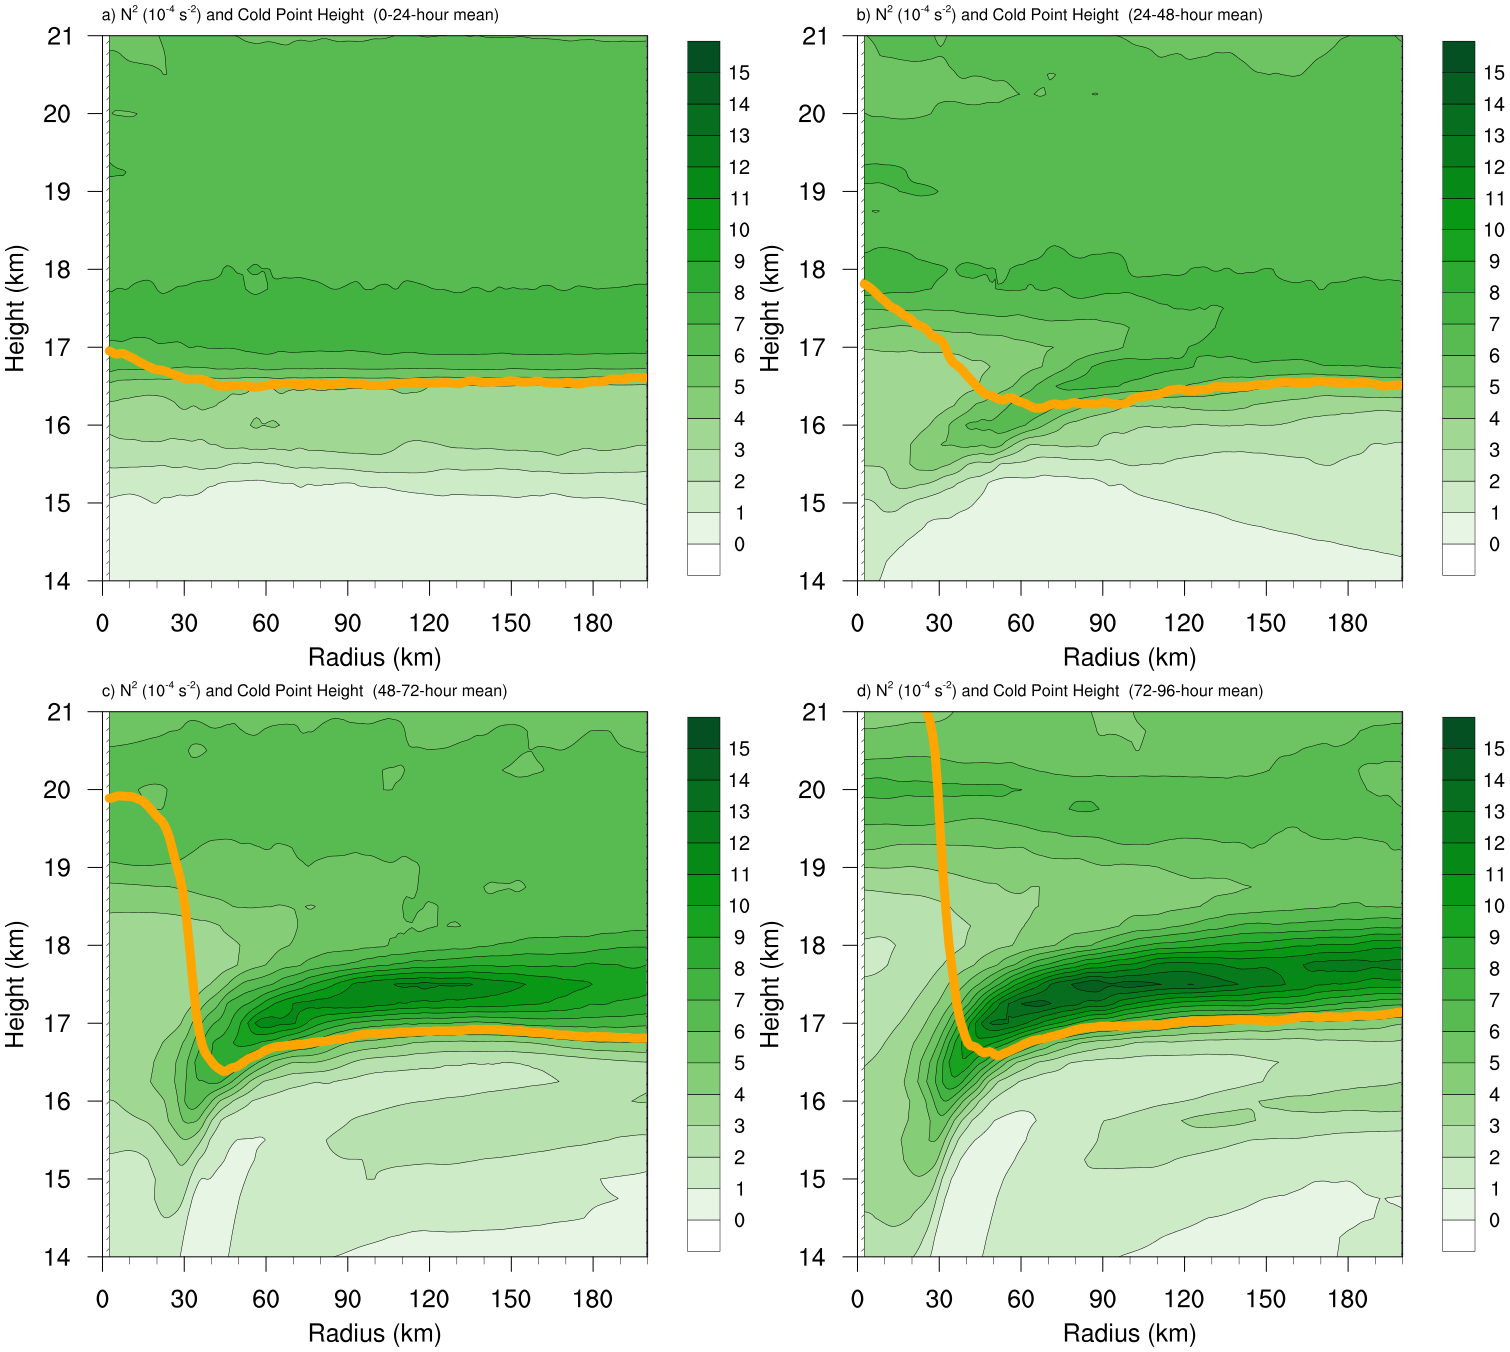
\includegraphics[width=39pc]{figures/n2-1000km.png}}
%\appendcaption{A1}{Twenty-four-hour averages of squared Brunt-V{\"a}is{\"a}l{\"a} frequency ($N^2$; 10\textsuperscript{-4} s\textsuperscript{-2}) over (a) 0-24 hours, (b) 24-48 hours, (c) 48-72 hours, and (d) 72-96 hours for the simulation described in Appendix Aa. Orange lines represent the cold-point tropopause height averaged over the same time periods.}
%\label{fig:n2-1000km}
%\end{figure*}
%
%%FIGURE A2%
%\begin{figure*}[ht]
%\centerline{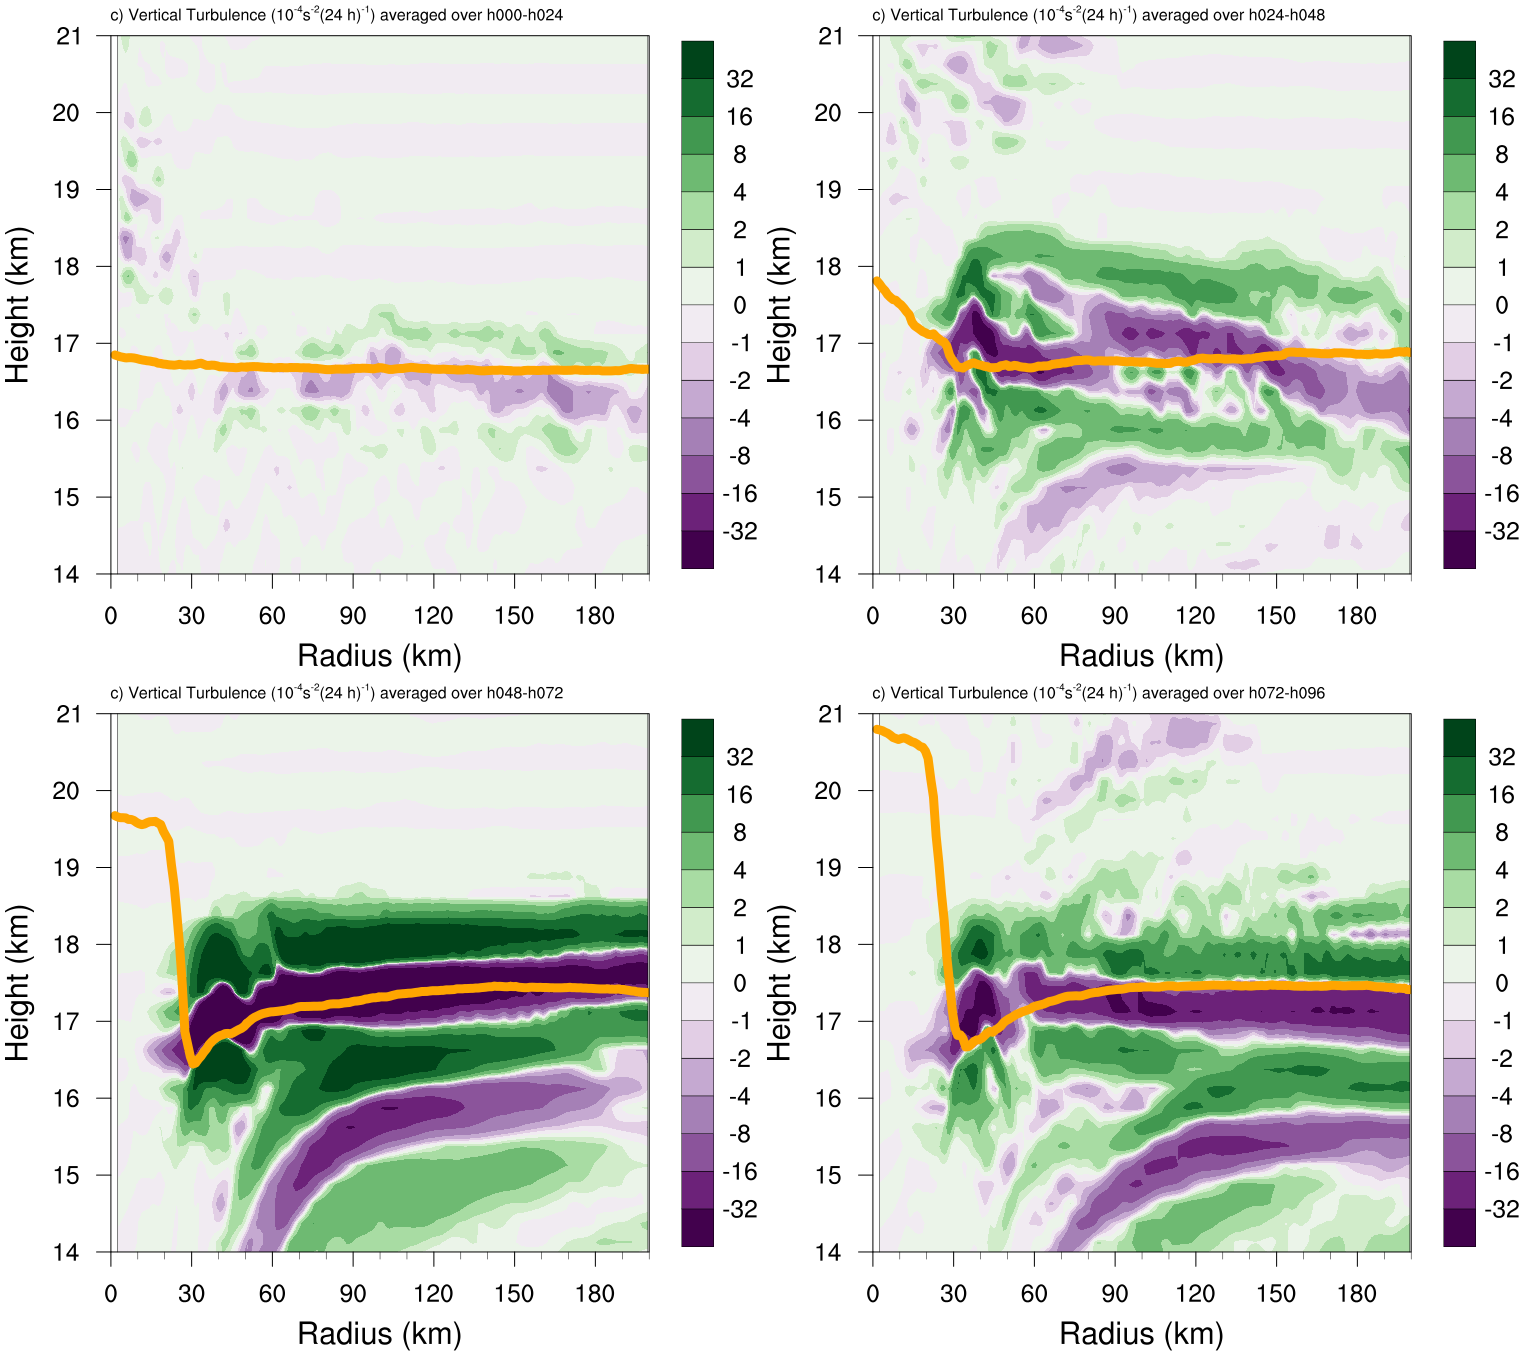
\includegraphics[width=39pc]{figures/turb-50m.png}}
%\appendcaption{A2}{The contribution of vertical turbulence to the $N^2$ variability (10\textsuperscript{-4} s\textsuperscript{-2} (24 h)\textsuperscript{-1}) averaged over (a) 0-24 hours, (b) 24-48 hours, (c) 48-72 hours, and (d) 72-96 hours for the simulation described in Appendix Ab. Orange lines represent the cold-point tropopause height averaged over the same time periods.}
%\label{fig:turb-50m}
%\end{figure*}

%\begin{figure}[t]
%\begin{figure}[t]
%\begin{figure}[t]
%  \noindent\includegraphics[width=19pc,angle=0]{figure01.pdf}\\
%  \caption{Enter the caption for your figure here.  Repeat as
%  necessary for each of your figures. Figure from \protect\cite{Knutti2008}.}\label{f1}
%\end{figure}


%%%%%%%%%%%%%%%%%%%%%%%%%%%%%%%%%%%%%%%%%%%%%%%%%%%%%%%%%%%%%%%%%%% 
%                                                                 %
%                           CHAPTER 5                             %
%                                                                 %
%%%%%%%%%%%%%%%%%%%%%%%%%%%%%%%%%%%%%%%%%%%%%%%%%%%%%%%%%%%%%%%%%%% 
 
\chapter{The tropopause-layer static stability structure of tropical cyclones as revealed by HS3 dropsondes and a large rawinsonde dataset}
\label{chapter:hs3}
\resetfootnote %this command starts footnote numbering with 1 again.

%---------------------------------------------------------------------------------------%
\section{Introduction}
%---------------------------------------------------------------------------------------%

The preceding two chapters documented the static stability evolution within extraordinarily intense TCs from both an observational and numerical modeling perspective.
The question remains, however, whether these results can be generalized to a large number of TCs at a range of intensities.
This chapter first documents the presence of large horizontal gradients of static stability observed within category-one Hurricane Nadine (2012) during the NASA Hurricane and Severe Storm Sentinel (HS3; \citeauthor{Braunetal2016} \citeyear{Braunetal2016}).
Then the static stability structure of a large number of TCs is analyzed using the same rawinsonde dataset as that employed in Chapter 2.

%---------------------------------------------------------------------------------------%
\section{Data and methods}
%---------------------------------------------------------------------------------------%
Hurricane Nadine (2012), a long-lived TC in the North Atlantic, was the focus of five research flights conducted by a NASA Global Hawk aircraft during HS3 \citep{Braunetal2016}.
The second research flight into the storm deployed 70 dropsondes \citep{Young2016} while Nadine intensified from a tropical storm to a category-one hurricane \citep{Brown2013} on 14 September 2012.
These dropsondes, deployed from the lower stratosphere, provided full-tropospheric profiles of temperature, humidity, and wind across a broad region of the storm.
The observations were interpolated to a 100-m vertical grid following \cite{MolinariVollaro2010} and the static stability ($N^2$) was computed following \cite{DuranMolinari2018}.
A great strength of the HS3 dropsonde dataset is that it provides numerous high-resolution soundings within and around individual TCs during short time periods.
This strength will be leveraged to analyze the tropopause-layer static stability structure of Nadine as it intensified to hurricane strength.

Although HS3 deployed 965 dropsondes within 1000 km of TCs over three years, providing unprecedented dropsonde coverage in TCs, these dropsondes sampled only seven different storms.
Thus, although numerous observations are available, these observations may not be representative of TCs in general.
To get a more general sense of the tropopause-layer structure of TCs, the large rawinsonde dataset of \cite{DuranMolinari2016} will be employed.
This dataset includes 11735 rawinsondes that were launched within 1000 km of TCs between the years 1998--2011\footnote{Note that fewer rawinsondes were included in the \cite{DuranMolinari2016} study because the Richardson number, which was the focus of that paper, requires both winds and thermodynamic observations. Many soundings were excluded from that analysis due to missing wind observations in the upper troposphere.}.
After imposing a requirement that the cold-point tropopause be located at or above 14 km, 9318 soundings remained within 1000 km of TCs.
These rawinsondes were deployed from stations across the eastern and central United States, as well as Belize, Grand Cayman, Puerto Rico, and Barbados (Fig. \ref{fig:maps}a).
They observed 164 different Atlantic-basin TCs at a wide range of intensities within the western Atlantic Ocean, Caribbean Sea, and the Gulf of Mexico (Fig. \ref{fig:maps}b).
Since most of the observations were collected over the mainland United States, the northwest quadrant of TCs was better-observed than other quadrants (Fig. \ref{fig:scatterplot}), particularly in hurricanes.
All quadrants, however, contained observations at a wide range of radii for all storm categories, which facilitates the construction of composite averages.

%---------------------------------------------------------------------------------------%
\section{Results}
%---------------------------------------------------------------------------------------%
\subsection{The tropopause-layer static stability structure of Hurricane Nadine (2012)}
The NASA Global Hawk aircraft completed multiple dropsonde transects across TC Nadine (2012) soon after it intensified to hurricane strength near 30\textdegree{}N latitude.
Observations from three dropsondes deployed during one of these transects are depicted in Fig. \ref{fig:nadine-skewt}.
One dropsonde was released near the edge of Nadine's cirrus canopy (Fig. \ref{fig:nadine-skewt}a, magenta star), a second within Nadine's cirrus canopy near cloud tops colder than -40\textdegree{}C (Fig. \ref{fig:nadine-skewt}a, green star), and a third within a region of cloud tops colder than -60\textdegree{}C (Fig. \ref{fig:nadine-skewt}b, blue star).
Temperature soundings from these three dropsondes are depicted in Fig. \ref{fig:nadine-skewt}b, where the colors of the lines correspond to the colors of the stars in Fig. \ref{fig:nadine-skewt}a).

All three soundings were fairly similar below the 200-mb level, but the temperature profiles differed considerably above that level.
The 150-200-mb layer was warmer on the edge of the cirrus canopy (magenta) than within the cirrus canopy (green, blue).
Both soundings deployed within the cirrus canopy (green, blue) exhibited very similar temperature profiles in this layer, with nearly dry-adiabatic lapse rates.
Just above the 150-mb layer, the sounding deployed within the coldest cloud tops (blue) exhibited a temperature inversion.
The other cirrus-canopy sounding (green) also exhibited a temperature inversion, but it was at a higher altitude than that observed within the region of coldest cloud tops (blue).
The difference in the height of these inversion layers corresponded to a maximum temperature difference of 4 K within this layer.
Above the inversion layers, however, the two soundings converged and exhibited very similar temperature profiles, including a nearly-identical cold point that was slightly warmer than that observed on the edge of the cirrus canopy (magenta).
These soundings indicate that strong horizontal gradients of temperature and stability existed in the upper levels of Hurricane Nadine.

Cross sections of squared Brunt-V{\"a}is{\"a}l{\"a} frequency ($N^2$; 10\textsuperscript{-4} s\textsuperscript{-2}) constructed using two sets of dropsondes are shown in Fig. \ref{fig:nadine-n2}.
The first set consisted of dropsondes (Fig. \ref{fig:nadine-n2}a) that were deployed primarily within and near Nadine's cirrus canopy.
The other set of dropsondes was released outside of Nadine's cirrus canopy, upshear of the center of circulation\footnote{According to the Statistical Hurricane Intensity Prediction Scheme (SHIPS; \citeauthor{DeMariaetal2005} \citeyear{DeMariaetal2005}) developmental database, the area-averaged, vortex-removed 850--200-mb wind shear at 00 UTC 15 September was 23 kt from the southwest.}.
The cross-sections are constructed along the flight track, with each of the dropsonde deployment locations marked by bold black digits on the satellite images and along the horizontal axes of the cross sections.

The dropsondes deployed within Nadine's cirrus canopy (Fig. \ref{fig:nadine-n2}a,b) detected two distinct static stability maxima in the 12--17-km layer.
One maximum was associated with a rapid increase in $N^2$ above the cold-point tropopause, which was located near the 16-km level.
This stability maximum is quite similar to that observed outside of the eye in Hurricane Patricia \citep{DuranMolinari2018} and is consistent with the tropopause inversion layer noted by \cite{Wirth2003}.
The second existed within the 13.5--15-km layer, where a horizontally-extended region of enhanced static stability was present everywhere within Nadine's cirrus canopy.
Within this lower stable layer, $N^2$ was largest in the two soundings that were deployed at locations where the infrared brightness temperature was colder than -55\textdegree{}C (dropsondes 4 and 7).
The static stability also maximized at a slightly higher altitude in these two soundings (14.4 and 14.5 km) than in the other soundings, which showed an $N^2$ maximum closer to 14 km.

The dropsondes deployed outside of Nadine's cirrus canopy (Fig. \ref{fig:nadine-n2}c,d) observed a considerably different upper-level static stability structure.
The lower-stratospheric $N^2$ maximum observed near and above 16 km was not nearly as coherent as it was within the cirrus canopy.
There existed numerous local $N^2$ maxima near and above 16 km, but rather than forming a horizontally-homogeneous stability maximum above the tropopause, the maxima were isolated from one another.
Likewise, there were a few weak, isolated local maxima in $N^2$ within the 12-15-km layer, but the distinct secondary stable layer that was observed within the cirrus canopy did not exist outside of the cirrus canopy.

These observations suggest that there might be processes unique to the TC cirrus canopy that produce stronger static stability above the cold-point tropopause and a secondary stability maximum below the tropopause.

\subsection{The relationship between infrared brightness temperature and the tropopause-layer temperature profile observed by HS3 dropsondes}
\label{hs3-irbt}

To get a more general sense of the relationship between infrared brightness temperature and the upper-tropospheric static stability structure, all HS3 dropsondes deployed within 500 km of TCs were analyzed.
The locations of these dropsondes relative to a composite TC center can be seen in Fig. \ref{fig:hs3-scatterplot}.
Only 26 of these observations were collected in tropical depressions, whereas 296 and 241 were collected in tropical storms and hurricanes, respectively.
The highest dropsonde density was within the innermost 100 km, but all radial bands and storm quadrants were sampled.
Each of these dropsondes was assigned an infrared brightness temperature by picking the satellite image pixel closest to the dropsonde deployment in both space and time, using 4-km-resolution GOES-13 infrared satellite imagery obtained from the NOAA Comprehensive Large Array-data Stewardship System (CLASS; \url{http://www.class.ncdc.noaa.gov/}).
The soundings were plotted on skew $T$--log $p$ diagrams and each sounding was assigned subjectively one of three classifications based on the upper-level temperature profile\footnote{These assignments were performed with no knowledge of the geographic location of the sounding, its location relative to a TC, or its infrared brightness temperature environment.}.
Examples of each of the three classifications are plotted in Fig. \ref{fig:skewt-examples}.
The "smooth tropopause" soundings (Fig. \ref{fig:skewt-examples}a) exhibited a temperature profile that transitioned smoothly from the upper troposphere to the lower stratosphere, whereas the "sharp tropopause" soundings (Fig. \ref{fig:skewt-examples}b) exhibited an abrupt transition near the tropopause.
The "multiple stable layer" soundings exhibited multiple distinct static stability maxima in the upper troposphere, as indicated by oscillations in the temperature profile (Fig. \ref{fig:skewt-examples}c).
If a profile exhibited multiple stable layers in the upper troposphere as well as a "sharp tropopause," the sounding was assigned the "multiple stable layer" classification.

Cumulative distributions of infrared brightness temperature for each of the three categories are plotted in Fig. \ref{fig:cdf}.
The distributions for the "sharp tropopause" (orange) and "multiple stable layer" (blue) categories are nearly identical, which indicates that sharp tropopauses and multiple stable layers tend to occur in regions of similar infrared brightness temperature.
These distributions also indicate that smooth tropopauses (red) tend to be located in regions of warmer infrared brightness temperature.
For example, 42\% of "sharp tropopause" soundings and 45\% of multiple stable layer soundings were located in regions with brightness temperatures colder than -40\textdegree{}C, whereas only 28\% of "smooth tropopause" soundings were located in such regions.
These distributions provide further evidence for a relationship between the infrared brightness temperature and the structure of the upper-tropospheric temperature profile.

\subsection{The tropopause-layer temperature structure of TCs as observed by a large rawinsonde dataset}

To get a general view of the tropopause-layer temperature structure in TCs, all rawinisondes shown in Fig. \ref{fig:scatterplot} are combined to create composite averages with respect to the cold-point tropopause.
These averages will be used to analyze the sensitivity of the tropopause-layer thermodynamic structure to TC intensity and cirrus environment.

\subsubsection{Sensitivity of the tropopause-layer thermodynamic structure to TC intensity}
First, soundings released in tropical depressions and tropical storms (blue and orange dots in Fig. \ref{fig:scatterplot}) are gathered into one category (hereafter called "weak TCs") and compared to hurricanes (red dots in Fig. \ref{fig:scatterplot}).
Composite averages of temperature, the vertical temperature gradient, and the second derivative of temperature with respect to height for these two intensity categories are plotted in Fig. \ref{fig:tline-int}.
For clarity, these plots focus on the 3-km-deep layers immediately surrounding the tropopause, with zero on the vertical axis corresponding to the tropopause height.

The tropopause-layer temperature in hurricanes (Fig. \ref{fig:tline-int} left, red line) is colder than in tropical depressions and tropical storms (Fig. \ref{fig:tline-int} left, blue line).
Although the composite-average temperatures for both categories are nearly identical 3 km below the tropopause, the two temperature profiles diverge with height up to the tropopause, where the average temperature in hurricanes is -75.8\textdegree{}C and in weak TCs -73.5\textdegree{}C.
This divergence in the temperature profiles corresponds to a steeper vertical temperature gradient below the tropopause in hurricanes than in weak TCs (Fig. \ref{fig:tline-int}, center), which is consistent with the smaller upper-tropospheric static stability observed in hurricanes by \cite{DuranMolinari2016}.
Curiously, the composite-average temperature in hurricanes remains colder than that in weak TCs all the way past 3 km above the tropopause, although the temperature difference decreases with height.
The convergence of the temperature profiles with height above the tropopause corresponds to a larger lower-stratospheric vertical temperature gradient in hurricanes than in weak TCs (Fig. \ref{fig:tline-int}, center), which suggests that hurricanes are characterized by stronger static stability in the lower stratosphere.
These results show that the effect of hurricanes on the thermodynamic environment is not limited to the troposphere; rather, their effects can extend far above the tropopause.

The second derivative of temperature with respect to height (Fig. \ref{fig:tline-int}, right) can be thought of as a measure of the "sharpness" of the tropopause.
Although this quantity is nearly identical in hurricanes and weak TCs throughout most of the tropopause layer, it is larger in hurricanes at and just above the tropopause than in weak TCs.
This shows that, on average, the tropopause is sharper (i.e., the vertical temperature gradient changes more rapidly with height) at the tropopause in hurricanes than in weak TCs.

\subsubsection{Sensitivity of the tropopause-layer thermodynamic structure to the infrared brightness temperature environment}
The HS3 observations shown in Section \ref{hs3-irbt} suggested that there might be some connection between the upper-tropospheric thermodynamic structure and the cloud environment.
To assess this potential connection in a larger number of storms, each rawinsonde in the dataset is assigned an infrared brightness temperature based on its location and time of release.
The brightness temperatures come from the GridSat-B1 Climate Data Record (CDR), which is a calibrated infrared brightness temperature dataset with 8-km resolution \citep{Knappetal2011}.
Although GridSat's relatively coarse resolution precludes observation of the coldest cloud tops in TCs associated with individual overshooting updrafts (e.g. \citeauthor{Griffin2017} \citeyear{Griffin2017}), its resolution is sufficient to discriminate between cloud-free areas and mesoscale regions of very cold cloud tops.

The rawinsondes are stratified into three bins according brightness temperature: colder than -50\textdegree{}C (Fig. \ref{fig:tline-ir}, magenta lines), between -30\textdegree{}C and -50\textdegree{}C (Fig. \ref{fig:tline-ir}, red lines), and warmer than -30\textdegree{}C (Fig. \ref{fig:tline-ir}, blue lines).
The left panel of Fig. \ref{fig:tline-ir} indicates that the colder the infrared brightness temperature in which the rawinsonde was released, the colder the upper-tropospheric and lower-stratospheric temperature observed by that rawinsonde.
Above the tropopause, the temperature differences are nearly constant with height, which is reflected in the very similar vertical temperature gradients observed for each of the categories (Fig. \ref{fig:tline-ir}, center panel).
These results suggest that deep convection within TCs alters the vertical temperature profile not only in the troposphere, but also well into the lower stratosphere.
The second derivative of temperature with respect to height (Fig. \ref{fig:tline-ir}, right panel) also indicates that regions with colder infrared brightness temperatures are characterized by a sharper tropopause.
This result is consistent with the subjective analysis conducting using HS3 dropsondes in Section \ref{hs3-irbt}.

%---------------------------------------------------------------------------------------%
\section{Discussion and ongoing work}
\label{sec:discussion}
%---------------------------------------------------------------------------------------%
In summary, the large rawinsonde dataset of \cite{DuranMolinari2016} reveals that not only do TCs affect the tropopause layer, but they also modify the thermodynamic profile well into the lower stratosphere.
These results are consistent with previous papers (e.g. \citeauthor{KuangBretherton2004} \citeyear{KuangBretherton2004}; \citeauthor{Salbyetal2003} \citeyear{Salbyetal2003}) that highlight the lower-stratospheric cooling effect of large-scale tropical convection.
Since tropopause height and lower-stratospheric temperature are a function of latitude (e.g. \citeauthor{HighwoodHoskins1998} \citeyear{HighwoodHoskins1998}), a next step would be to investigate whether the TC tropopause structure differs between high-latitude TCs and low-latitude TCs.
%It is possible that upper-tropospheric double stable layers like those observed in Hurricane Nadine (2012; see Fig. \ref{fig:nadine-n2}b) are more common at higher latitudes than at lower latitudes.

The rawinsonde observations also reveal that regions of colder cloud tops are characterized by a sharper tropopause than regions of warmer cloud tops or regions devoid of cloud.
These results confirm the conclusions of the subjective analysis that was described in Section \ref{hs3-irbt} using the HS3 dropsonde dataset.
To confirm the presence of multiple stable layers in regions of cold cirrus, an objective algorithm is currently under development to detect multiple stability maxima in the tropopause layer.

%---------------------------------------------------------------------------------------%
%FIGURES AND TABLES
%---------------------------------------------------------------------------------------%

%FIGURE 1%
\begin{figure*}[ht]
\centerline{\includegraphics[width=33pc]{figures/stationmap+stormlocations.png}}
\caption{(top) Map of the number of rawinsondes deployed by stations located within 1000 km of tropical cyclone center positions. (bottom) The locations of the center positions of (blue stars) tropical depressions, (orange stars) tropical storms, and (red stars) hurricanes at times when rawinsonde observations were collected.}
\label{fig:maps}
\end{figure*}

%FIGURE 2%
\begin{figure*}[ht]
\centerline{\includegraphics[width=39pc]{figures/droplocs_scatterplot_rawinsondes.png}}
\caption{Rawinsonde deployment locations relative to a composite TC center for (blue) tropical depressions, (orange) tropical storms, and (red) hurricanes. Range rings are plotted every 100 km, starting at 100 km and ending at 1000 km.}
\label{fig:scatterplot}
\end{figure*}

%FIGURE 3%
\begin{figure*}[ht]
\centerline{\includegraphics[width=39pc]{figures/nadine-skewt.png}}
   \caption{(a) Infrared brightness temperature (\textdegree{}C) image of Hurricane Nadine at 2245 UTC 14 September 2012. Magenta, green, and blue stars represent dropsonde deployment locations corresponding to the three temperature soundings shown in (b) the skew $T$--log $p$ diagram.}
\label{fig:nadine-skewt}
\end{figure*}

%FIGURE 4%
\begin{figure*}[ht]
\centerline{\includegraphics[width=39pc]{figures/nadine-n2}}
   \caption{Infrared brightness temperature (\textdegree{}C) images of Hurricane Nadine at (a) 2315 UTC 14 September 2012 and (c) 0015 UTC 15 September 2015. Digits represent dropsonde deployment locations. (b,d) Vertical cross sections of the squared Brunt-V{\"a}is{\"a}l{\"a} frequency ($N^2$; 10\textsuperscript{-4} s\textsuperscript{-2}) constructed using the dropsondes depicted in the left panels. Digits along the bottom of the cross-sections correspond to the dropsonde locations indicated in (a) and (c).}
\label{fig:nadine-n2}
\end{figure*}

%FIGURE 5%
\begin{figure*}[ht]
\centerline{\includegraphics[width=39pc]{figures/droplocs_scatterplot_hs3.png}}
\caption{As in Fig. \ref{fig:scatterplot}, but for all dropsondes deployed within 500 km of a TC center during the NASA Hurricane and Severe Storm Sentinel field campaign.}
\label{fig:hs3-scatterplot}
\end{figure*}

%FIGURE 6%
\begin{figure*}[ht]
\centerline{\includegraphics[width=39pc]{figures/skewt-examples.png}}
\caption{Skew $T$--log $p$ diagrams depicting examples of three tropopause structure classifications: (top left) smooth tropopause, (top right) sharp tropopause, (bottom left) multiple stable layer.}
\label{fig:skewt-examples}
\end{figure*}

%FIGURE 7%
\begin{figure*}[ht]
\centerline{\includegraphics[width=27pc]{figures/tb_cdf_10Cbins_0-500km.png}}
\caption{Cumulative distributions of infrared brightness temperature (\textdegree{}C) for three tropopause structure classifications: (red) smooth tropopause, (orange) sharp tropopause, and (blue) multiple stable layer.}
\label{fig:cdf}
\end{figure*}


%FIGURE 8%
\begin{figure*}[ht]
\centerline{\includegraphics[width=39pc]{figures/t+dtdz+d2tdz2-intensity-montage.png}}
\caption{Composite-mean vertical profiles of (left) temperature (\textdegree{}C), (middle) the vertical temperature gradient (\textdegree{}C km\textsuperscript{-1}), and (right) the second derivative of temperature with respect to height (\textdegree{}C km\textsuperscript{-2}) composited about the cold-point tropopause height for (blue) tropical depressions and tropical storms and (red) hurricanes.}
\label{fig:tline-int}
\end{figure*}

%FIGURE 9%
\begin{figure*}[ht]
\centerline{\includegraphics[width=39pc]{figures/t+dtdz+d2tdz2-irbt-montage.png}}
\caption{As in Fig. \ref{fig:tline-int} but for rawinsondes deployed in regions of brightness temperature (magenta) colder than -50\textdegree{}C, (red) between -30 and -50\textdegree{}C, and (blue) warmer than -30\textdegree{}C.}
\label{fig:tline-ir}
\end{figure*}


%\include{conclusions}
% ...
% Add new \include{chapterX} statements for each chapter you add
%%%%%%%%%%%%%%%%%%%%%%%%%%%%%%%%%%%%%%%%%%%%%%%%%%%%%%%%%%%%%%%%%%%% 
%                                                                 %
%                           CHAPTER 5                             %
%                                                                 %
%%%%%%%%%%%%%%%%%%%%%%%%%%%%%%%%%%%%%%%%%%%%%%%%%%%%%%%%%%%%%%%%%%% 
 
\chapter{Permission to use copyrighted material from the American Meteorological Society}
\label{chapter:appendix}
\resetfootnote %this command starts footnote numbering with 1 again.

\begin{figure*}[ht]
\centerline{\includegraphics[width=39pc]{figures/AMSpermission.png}}
%\caption{As in Fig. \ref{fig:dist-pert}, but at 0000 UTC (solid lidnes) and 1200 UTC (dotted lines).}
\label{fig:amspermission}
\end{figure*}

\end{doublespace}
%\printglossaries

\bibliographystyle{ametsoc}  %need ametsoc.bst in the directory you run this
\bibliography{references}  %path to references.bib file

\end{document}
